% #############################################################################
% Main document of the dissertation
% Structure follows the IST Thesis-MSc template (Version 4, August 2022, by
% Prof. Rui Santos Cruz)
% !TEX root = ./Main.tex
% #############################################################################
\documentclass[defaultstyle,10pt,Helvetica,twoside,openright]{Thesis}
% #############################################################################
% Preamble of the dissertation
% Styling follows the IST Thesis-MSc template (Version 4, August 2022, by
% Prof. Rui Santos Cruz); only the packages this document uses are loaded.
% !TEX root = ./Main.tex
% #############################################################################
%
% -----------------------------------------------------------------------------
% Encoding and language
% -----------------------------------------------------------------------------
\usepackage[utf8]{inputenc}
\usepackage[T1]{fontenc}
\usepackage[main=english,portuguese]{babel}
\usepackage{iflang}
%
% -----------------------------------------------------------------------------
% Mathematics and figures
% -----------------------------------------------------------------------------
\usepackage{mathtools, amssymb}
\usepackage{tikz}
\usetikzlibrary{shapes.geometric, arrows, positioning}
%
% -----------------------------------------------------------------------------
% Tables
% -----------------------------------------------------------------------------
\usepackage{array}
\usepackage{booktabs}
\usepackage{tabularx}
\usepackage{makecell}
\usepackage{rotating}
%
% -----------------------------------------------------------------------------
% Captions
% -----------------------------------------------------------------------------
\usepackage[format=hang,labelfont=bf,font=small]{caption}
\captionsetup[table]{skip=10pt}
%
% -----------------------------------------------------------------------------
% Algorithms
% -----------------------------------------------------------------------------
\usepackage[ruled,vlined,algochapter,norelsize,\languagename]{algorithm2e}
\SetKwInput{KwRequire}{Require}
%
% -----------------------------------------------------------------------------
% Emphasis as underline, as in the IST template (restored to italics for the
% bibliography in Main.tex)
% -----------------------------------------------------------------------------
\usepackage[ULforem,normalbf]{ulem}
%
% -----------------------------------------------------------------------------
% Colours used by the chapter heads and the hyperlinks
% -----------------------------------------------------------------------------
\usepackage{xcolor}
\definecolor{darkgray}{rgb}{0.4, 0.4, 0.4}
\definecolor{chaptergrey}{rgb}{0.6,0.6,0.6}
%
% -----------------------------------------------------------------------------
% Line spacing
% -----------------------------------------------------------------------------
\usepackage{setspace}
%
% -----------------------------------------------------------------------------
% Citations, acronyms, hyperlinks and cross-references
% -----------------------------------------------------------------------------
\usepackage{cite}
\usepackage[nohyperlinks]{acronym}
\usepackage{hyperref}
\hypersetup{ colorlinks=true,
             citecolor=cyan,
             linkcolor=darkgray,
             urlcolor=teal,
             breaklinks=true,
             bookmarksnumbered=true,
             bookmarksopen=true,
}
\usepackage{url}
\usepackage[\IfLanguageName{english}{english}{brazilian}]{cleveref}
%
% -----------------------------------------------------------------------------
% Lists
% -----------------------------------------------------------------------------
\usepackage[shortlabels]{enumitem}
\setlist[description]{leftmargin=\parindent,labelindent=\parindent,itemsep=1pt,parsep=0pt,topsep=0pt}
%
% -----------------------------------------------------------------------------
% Glossary, sorted by LaTeX itself so no external indexing tool is needed
% -----------------------------------------------------------------------------
\usepackage[nopostdot,nonumberlist]{glossaries}
\makeatletter
\newglossarystyle{mystyle}{%
  \setglossarystyle{altlist}%
  \renewenvironment{theglossary}{%
  \begin{description}[style=standard,labelindent=0pt,itemsep=5pt]%
  }%
  {\end{description}}
  \renewcommand*{\glossentry}[2]{%
    \item[\glsentryitem{##1}%
      \glstarget{##1}{\glossentryname{##1}}]%
      \mbox{}\par\nobreak\@afterheading
      \glossentrydesc{##1}\glspostdescription%
  }%
  \renewcommand{\glsgroupskip}{}%
}
\makeatother
\setglossarystyle{mystyle}
\makenoidxglossaries
% #############################################################################
% Glossary entries, in alphabetical order
% !TEX root = ../../Main.tex
% #############################################################################
\newglossaryentry{alpha}
{
    name=alpha,
    description={The part of a strategy's mean return that its exposure to the market does not explain, taken from the regression of the strategy's returns on the market's returns}
}
\newglossaryentry{ask}
{
    name=ask price,
    description={The price at which the market sells, paid to open a long position or to close a short one}
}
\newglossaryentry{backtest}
{
    name=backtest,
    description={A simulation of a trading strategy on historical prices}
}
\newglossaryentry{balance}
{
    name=balance,
    description={The account value from closed positions only, before the result of any open position}
}
\newglossaryentry{base}
{
    name=base currency,
    description={The first currency of a pair, the one being bought or sold; the pair's price is the amount of quote currency one unit of it costs}
}
\newglossaryentry{beta}
{
    name=beta,
    description={The sensitivity of a strategy's return to the market's return, the slope of the regression of one on the other}
}
\newglossaryentry{bid}
{
    name=bid price,
    description={The price at which the market buys, received when closing a long position or opening a short one}
}
\newglossaryentry{calmar}
{
    name=Calmar ratio,
    description={The annualised return divided by the maximum drawdown}
}
\newglossaryentry{commission}
{
    name=commission,
    description={The fee a broker charges for the volume traded, on opening and on closing a position}
}
\newglossaryentry{pair}
{
    name=currency pair,
    description={The price of one currency expressed in another, such as EUR/USD}
}
\newglossaryentry{drawdown}
{
    name=drawdown,
    description={The fall of equity from its previous peak, as a fraction of that peak}
}
\newglossaryentry{equity}
{
    name=equity,
    description={The balance plus the unrealised result of the open positions}
}
\newglossaryentry{hedging}
{
    name=hedging account,
    description={An account that can hold several positions on one instrument, in either direction, at the same time}
}
\newglossaryentry{leverage}
{
    name=leverage,
    description={The ratio between the size of a position and the account capital that backs it}
}
\newglossaryentry{long}
{
    name=long position,
    description={A position that gains when the price rises}
}
\newglossaryentry{lot}
{
    name=lot,
    description={A standard trade size of 100,000 units of the base currency}
}
\newglossaryentry{netting}
{
    name=netting account,
    description={An account that holds at most one position per instrument, so an opposite order reduces, closes or reverses it}
}
\newglossaryentry{pip}
{
    name=pip,
    description={The fourth decimal place of most currency pair prices, and the second for pairs quoted in Japanese yen}
}
\newglossaryentry{quote}
{
    name=quote currency,
    description={The second currency of a pair, in which the price is expressed}
}
\newglossaryentry{sharpe}
{
    name=Sharpe ratio,
    description={The mean excess return divided by the standard deviation of returns}
}
\newglossaryentry{short}
{
    name=short position,
    description={A position that gains when the price falls}
}
\newglossaryentry{sortino}
{
    name=Sortino ratio,
    description={The mean excess return divided by the standard deviation of the negative returns only}
}
\newglossaryentry{spread}
{
    name=spread,
    description={The difference between the ask and the bid prices, paid on every round trip}
}
\newglossaryentry{swap}
{
    name=swap,
    description={The interest charged or paid for holding a position past the daily rollover time}
}
\newglossaryentry{tick}
{
    name=tick,
    description={A single change in the quoted ask or bid price}
}
\newglossaryentry{walkforward}
{
    name=walk-forward analysis,
    description={An evaluation in which a model is trained on one period and scored on the following one, repeated as the periods move forward in time}
}
\glsaddall
%
% #############################################################################
% GLOBAL FORMATTING OF THE THESIS DOCUMENT (IST template, unchanged)
% #############################################################################
\usepackage{./Cover}
%
% Paragraph counter in alphanumeric mode, as the IST guide requires
\renewcommand{\theparagraph}{\Alph{paragraph}~--}
\hoffset 0in
\voffset 0in
\oddsidemargin 0 cm
\evensidemargin 0 cm
\marginparsep 0in
\topmargin -0.25cm
\textwidth 16 cm
\textheight 22.4 cm
\makeatletter
\def\@afterindentfalse{\let\if@afterindent\iffalse}
\makeatother
%
% -----------------------------------------------------------------------------
% Headers and footers
% -----------------------------------------------------------------------------
\usepackage{fancyhdr}
\pagestyle{fancy}
\renewcommand{\chaptermark}[1]{\markboth{\thechapter.\ #1}{}}
\renewcommand{\sectionmark}[1]{\markright{\thesection\ #1}}
\fancyhf{}
\fancyfoot[C]{\bfseries\thepage}
\renewcommand{\headrulewidth}{0.0pt}
\renewcommand{\footrulewidth}{0.0pt}
\addtolength{\headheight}{2pt}
\fancypagestyle{plain}{%
   \renewcommand{\headrulewidth}{0pt}
   \renewcommand{\footrulewidth}{0pt}
}
\fancypagestyle{blank}{%
   \renewcommand{\headrulewidth}{0pt}
   \renewcommand{\footrulewidth}{0pt}
}
\fancypagestyle{abstract}{%
   \renewcommand{\headrulewidth}{0pt}
   \renewcommand{\footrulewidth}{0.0pt}
}
\fancypagestyle{document}{%
	\renewcommand{\headrulewidth}{0.5pt}
	\renewcommand{\footrulewidth}{0.5pt}
	\addtolength{\headheight}{2pt}
}
\setcounter{secnumdepth} {5}
\setcounter{tocdepth} {5}
\renewcommand{\thesubsubsection}{\thesubsection.\Alph{subsubsection}}
%
% -----------------------------------------------------------------------------
% Chapter heads with a mini table of contents (\fancychapter)
% -----------------------------------------------------------------------------
\usepackage{minitoc}
\setcounter{minitocdepth}{1}
\setlength{\mtcindent}{24pt}
\renewcommand{\mtcfont}{\small\rm}
\renewcommand{\mtcSfont}{\small\bf}
\renewcommand*{\kernafterminitoc}{\kern0.\baselineskip\kern0.ex}
\mtcselectlanguage{\languagename}
\makeatletter
\def\boxedverbatim{%
  \def\verbatim@processline{%
    {\setbox0=\hbox{\the\verbatim@line}%
    \hsize=\wd0 \the\verbatim@line\par}}%
  \@minipagetrue%
  \@tempswatrue%
  \setbox0=\vbox\bgroup\vspace*{0.2cm}\footnotesize\verbatim
}
\def\endboxedverbatim{%
  \endverbatim
  \unskip\setbox0=\lastbox%
  \hspace*{0.2cm}
  \vspace*{-0.2cm}
  \egroup
  \fbox{\box0}%
}
\makeatother
\newcommand*{\chapnumfont}{%
  \usefont{T1}{pbk}{b}{n}
  \fontsize{130}{100}
  \selectfont
  \color{chaptergrey}
}
\makeatletter
\def\@makechapterhead#1{%
  \vspace*{50\p@}%
  {\parindent \z@ \raggedright \normalfont
    {\chapnumfont\ifnum \c@secnumdepth >\m@ne
        \raggedleft\bfseries \thechapter
        \par\nobreak
        \vskip 20\p@
    \fi}
    \interlinepenalty\@M
    {\raggedleft\Huge \bfseries #1\par\nobreak}
    \vskip 40\p@
  }}
\makeatother
\newcommand{\fancychapter}[1]{\chapter{#1}\minitoc\bigskip}
%
% -----------------------------------------------------------------------------
% Official name of the degree (automatic for MEIC, depends on the language)
% -----------------------------------------------------------------------------
\IfLanguageName{english}
		{\degree{Computer Science and Engineering}}
		{\degree{Engenharia Informática e de Computadores}}
% #############################################################################
\begin{document}
%
% -----------------------------------------------------------------------------
% Cover and declaration
\pdfbookmark[0]{Titlepage}{Title}
% #############################################################################
% Cover page data
% !TEX root = ../../Main.tex
% #############################################################################
%
% University logo, 2 cm from the top and left page edges as IST requires
\univlogo{20mm}{20mm}{./Images/IstLogo}
%
% -----------------------------------------------------------------------------
% Title
\title{Deep Reinforcement Learning applied to Forex Market: Deep Deterministic Policy Gradient Trading System}
%
% -----------------------------------------------------------------------------
% Author
\author{Vicente Aser Marques Rebelo Castillo Lorenzo}
%
% -----------------------------------------------------------------------------
% Supervisor
\supervisor{Prof. Rui Fuentecilla Maia Ferreira Neves}
%
% -----------------------------------------------------------------------------
% Date of the examination (month and year)
\date{October 2026}
%
% -----------------------------------------------------------------------------
% The Examination Committee is printed; names are placeholders until approved
\finalthesis{true}
\chairperson{Prof. Name of the Chairperson}
\vogalone{Prof. Name of First Committee Member}
\maketitle
\thispagestyle{empty}
\cleardoublepage
%
% -----------------------------------------------------------------------------
% Front matter in roman numbering
\setcounter{page}{1} \pagenumbering{roman}
\baselineskip 18pt
\raggedbottom
%
% -----------------------------------------------------------------------------
% Acknowledgements
\pdfbookmark[0]{Acknowledgments}{acknowledgments}
\begin{acknowledgments}
	% #############################################################################
% Acknowledgements
% !TEX root = ../../Main.tex
% #############################################################################
\noindent [Acknowledgements to be written by the author.]
\end{acknowledgments}
%
% -----------------------------------------------------------------------------
% Abstract and keywords
\begin{abstract}
	% #############################################################################
% Abstract
% !TEX root = ../../Main.tex
% #############################################################################
\acresetall
\noindent Reinforcement learning for currency trading is usually tested on one pair, on bar data and without real costs. This thesis trains one Deep Deterministic Policy Gradient (DDPG) agent, with one design and no tuning per pair, on each of the seven major currency pairs, over eleven years of tick data from 2015 to 2025. The agent is implemented as in the original DDPG paper: an off-policy actor-critic with actor and critic networks, slowly updated target copies of both, a replay buffer and Ornstein-Uhlenbeck exploration noise, with the published hyperparameters where they apply. The actor maps 38 dimensionless features from sixteen technical indicators to one continuous action in $[-1, 1]$, whose sign sets the direction of the position and whose magnitude sets its size within a volatility-based risk budget. The critic learns the value of that action, and the reward is the log return of account equity. Four documented changes adapt it to this problem: smaller networks with layer normalisation, a penalty against output saturation, a scaled reward and mirrored training episodes. The agent is trained and evaluated in a tick-level backtesting engine, built for this work to reproduce cTrader's backtester, that replays 1.6 billion quotes and charges the real costs of a raw-spread, swap-free retail account: the spread quoted at each fill, a commission of 3.5 US dollars per lot per side and a swap of zero. Each pair is trained with an anchored walk-forward, the standard validation method for trading systems: seven folds validate on 2018 to 2024, 2025 is held out as the test year, and a model is kept only if it passes eleven checks on return and behaviour. All seven models are profitable net of all costs. They returned between \ResultStitchedMin{} and \ResultStitchedMax{} over the walk-forward years, between \ResultTestMin{} and \ResultTestMax{} in the held-out year and between \ResultFullMin{} and \ResultFullMax{} over the full period, with Sharpe ratios of \ResultSharpeMin{} to \ResultSharpeMax{} and a yearly alpha of \ResultAlphaMin{} to \ResultAlphaMax{}, and each beats its own pair in all three windows. As an equal-weight portfolio they returned \ResultPortfolioReturn{} against \ResultBenchmarkReturn{} for the US 500 index, with a maximum drawdown of \ResultPortfolioDrawdown{} against \ResultBenchmarkDrawdown{} and a Sharpe ratio of \ResultPortfolioSharpe{} against \ResultBenchmarkSharpe{}, because the seven models make and lose money at different times.

\end{abstract}
\begin{keywords}
	% #############################################################################
% Keywords
% !TEX root = ../../Main.tex
% #############################################################################
\acresetall
\noindent Forex Trading; Deep Reinforcement Learning; Deep Deterministic Policy Gradient; Transaction Costs; Portfolio Construction
\end{keywords}
\clearpage
\thispagestyle{empty}
\cleardoublepage
%
% -----------------------------------------------------------------------------
% Resumo and palavras-chave
\begin{resumo}
	% #############################################################################
% Resumo
% !TEX root = ../../Main.tex
% #############################################################################
\acresetall
\begin{otherlanguage}{portuguese}
\noindent A aprendizagem por reforço aplicada aos mercados cambiais é normalmente testada num único par, com dados em \textit{bars} e sem custos reais. Esta tese treina um agente Deep Deterministic Policy Gradient (DDPG), com um único desenho e sem ajustes por par, em cada um dos sete principais pares de moeda, com onze anos de dados ao \textit{tick}, de 2015 a 2025. O agente é implementado como no artigo original do DDPG: um método ator-crítico \textit{off-policy} com redes do ator e do crítico, cópias-alvo de ambas atualizadas lentamente, memória de repetição e ruído de exploração de Ornstein-Uhlenbeck, com os hiperparâmetros publicados onde se aplicam. O ator transforma 38 variáveis adimensionais, obtidas de dezasseis indicadores técnicos, numa única ação contínua em $[-1, 1]$, cujo sinal define a direção da posição e cuja magnitude define a sua dimensão, dentro de um orçamento de risco baseado na volatilidade. O crítico aprende o valor dessa ação, e a recompensa é o retorno logarítmico do capital. Quatro alterações documentadas adaptam-no a este problema: redes mais pequenas com normalização por camada, uma penalização contra a saturação da saída, uma recompensa escalada e episódios de treino espelhados. O agente é treinado e avaliado num motor de \textit{backtesting} ao \textit{tick}, construído para reproduzir o do cTrader, que percorre 1,6 mil milhões de cotações e cobra os custos reais de uma conta de retalho \textit{raw-spread} e \textit{swap-free}: o \textit{spread} de cada execução, uma comissão de 3,5 dólares americanos por lote e por lado e um \textit{swap} nulo. Cada par é treinado com uma validação \textit{walk-forward} ancorada, o método padrão para sistemas de negociação: sete partições validam de 2018 a 2024, 2025 é reservado como ano de teste, e cada modelo tem de passar onze critérios de retorno e comportamento. Os sete modelos são lucrativos após todos os custos. Obtiveram entre \ResultStitchedMinPT{} e \ResultStitchedMaxPT{} nos anos de validação, entre \ResultTestMinPT{} e \ResultTestMaxPT{} no ano de teste e entre \ResultFullMinPT{} e \ResultFullMaxPT{} no período completo, com rácios de Sharpe de \ResultSharpeMinPT{} a \ResultSharpeMaxPT{} e um alfa anual de \ResultAlphaMinPT{} a \ResultAlphaMaxPT{}, e cada um supera o seu par nos três períodos. Numa carteira de pesos iguais obtiveram \ResultPortfolioReturnPT{} contra \ResultBenchmarkReturnPT{} do índice US 500, com uma perda máxima de \ResultPortfolioDrawdownPT{} contra \ResultBenchmarkDrawdownPT{} e um rácio de Sharpe de \ResultPortfolioSharpePT{} contra \ResultBenchmarkSharpePT{}, porque os sete modelos ganham e perdem dinheiro em momentos diferentes.
\end{otherlanguage}

\end{resumo}
\begin{palavraschave}
	% #############################################################################
% Palavras-chave
% !TEX root = ../../Main.tex
% #############################################################################
\acresetall
\begin{otherlanguage}{portuguese}
\noindent Negociação Forex; Aprendizagem por Reforço Profunda; Deep Deterministic Policy Gradient; \textit{Backtesting}; Custos de Transação; Validação \textit{Walk-Forward}
\end{otherlanguage}
\end{palavraschave}
\clearpage
\thispagestyle{empty}
\cleardoublepage
%
% -----------------------------------------------------------------------------
% Mini tables of contents of each chapter
\dominitoc
\dominilof
\dominilot
%
% -----------------------------------------------------------------------------
% Contents, figures, tables and algorithms
\renewcommand{\baselinestretch}{1}
\pdfbookmark[0]{Contents}{toc}
\tableofcontents
\cleardoublepage
\renewcommand{\baselinestretch}{1.5}
\pdfbookmark[1]{List of Figures}{lof}
\listoffigures
\begingroup
\pdfbookmark[1]{List of Tables}{lot}
\listoftables
\pdfbookmark[1]{List of Algorithms}{loa}
\listofalgorithms
\endgroup
%
% -----------------------------------------------------------------------------
% Acronyms
\pdfbookmark[1]{Acronyms}{loac}
\chapter*{\tlangAcronyms}
% #############################################################################
% Acronyms, in alphabetical order
% !TEX root = ../../Main.tex
% #############################################################################
\begin{acronym}[OHLCV]
	\acro{A2C}{Advantage Actor-Critic}
	\acro{A3C}{Asynchronous Advantage Actor-Critic}
	\acro{ATR}{Average True Range}
	\acro{AUD}{Australian Dollar}
	\acro{CAD}{Canadian Dollar}
	\acro{CHF}{Swiss Franc}
	\acro{DDPG}{Deep Deterministic Policy Gradient}
	\acro{DDQN}{Double Deep Q-Network}
	\acro{DQN}{Deep Q-Network}
	\acro{DRL}{Deep Reinforcement Learning}
	\acro{DRQN}{Deep Recurrent Q-Network}
	\acro{EMA}{Exponential Moving Average}
	\acro{ER}{Efficiency Ratio}
	\acro{ETF}{Exchange-Traded Fund}
	\acro{EUR}{European Euro}
	\acro{FNN}{Feedforward Neural Network}
	\acro{GBP}{Great Britain Pound}
	\acro{GDPG}{Gated Deterministic Policy Gradient}
	\acro{GDQN}{Gated Deep Q-Network}
	\acro{GRU}{Gated Recurrent Unit}
	\acro{JPY}{Japanese Yen}
	\acro{LSTM}{Long Short-Term Memory}
	\acro{MACD}{Moving Average Convergence Divergence}
	\acro{MDP}{Markov Decision Process}
	\acro{MSE}{Mean Squared Error}
	\acro{NN}{Neural Network}
	\acro{NZD}{New Zealand Dollar}
	\acro{OHLCV}{Open, High, Low, Close and Volume}
	\acro{PPO}{Proximal Policy Optimisation}
	\acro{ReLU}{Rectified Linear Unit}
	\acro{RL}{Reinforcement Learning}
	\acro{RNN}{Recurrent Neural Network}
	\acro{ROC}{Rate of Change}
	\acro{RSI}{Relative Strength Index}
	\acro{RV}{Realised Volatility}
	\acro{SARSA}{State-Action-Reward-State-Action}
	\acro{SD}{Standard Deviation}
	\acro{SMA}{Simple Moving Average}
	\acro{TD}{Temporal Difference}
	\acro{TD3}{Twin Delayed Deep Deterministic Policy Gradient}
	\acro{USD}{US Dollar}
	\acro{WMA}{Weighted Moving Average}
\end{acronym}
\clearpage
%
% -----------------------------------------------------------------------------
% Glossary
\pdfbookmark[1]{Glossary}{glo}
\printnoidxglossary[]
\cleardoublepage
%
% -----------------------------------------------------------------------------
% Document matter in arabic numbering
\setcounter{page}{1} \pagenumbering{arabic}
\baselineskip 18pt
\flushbottom
%
\acresetall
% !TEX root = ../../Main.tex
\fancychapter{Introduction}
\label{Chapter:Introduction}

The foreign exchange market is the largest financial market in the world. In April 2025, its average turnover was 9.6 trillion US dollars per day \cite{bis_otc_2025}. It trades continuously from Sunday evening to Friday evening. This makes it a good target for automated trading. A program can trade at any hour. The major currency pairs absorb retail order sizes without moving the price. The price history is also available down to single quotes. However, there is little useful signal in the prices. Over short horizons, returns are close to unpredictable \cite{fama_efficient_1970}. The cost of trading is also high. Many strategies that look profitable in a simplified test lose money once these costs are charged.

This work applies Deep Reinforcement Learning (DRL) to this problem. One Deep Deterministic Policy Gradient (DDPG) \cite{lillicrap_continuous_2015} agent is trained for each of the seven major currency pairs. Each agent is evaluated over eleven years of tick data. The evaluation charges the spread quoted at the time of the trade and the commission of a retail account.

% !TEX root = ../../Main.tex
\section{Motivation}

Automated currency trading is usually built from fixed rules. Technical indicators are computed from recent prices. A signal is then taken from them, either by comparing them or by a crossover. A separate layer of the system decides the position size \cite{chan_quantitative_2021, brandimarte_introduction_2018}. These systems are cheap to run and easy to check, and this is why they are common. Their parameters are set once and do not change, so the system does not adapt when the market changes. This is the first of the two difficulties that this work deals with.

Currencies were chosen over equities for practical reasons \cite{donnelly_art_2019}. The market trades continuously on weekdays, so a position is never carried through a daily close during which it cannot be traded. There are only seven major pairs. This makes it possible to test a design on all of them, instead of on a sample chosen by the author. A trader can buy or sell with no borrowing cost and no short-selling restrictions. A policy that sells is therefore not penalised by market mechanics that have nothing to do with its signal. Every major pair also has the US dollar on one side. The seven instruments are therefore related, but one cannot replace another. A comparison of the results across them says something about the design and not about one price series.

Reinforcement learning describes the same task without splitting it into a prediction and an action. The agent observes the state of the market and chooses a position. It then receives the profit or loss of that position as its reward \cite{sutton_reinforcement_2018}. The agent never has to forecast a price. It only has to act. Its action is measured in money, which is also how a trading system is judged in practice.

DDPG fits this task well. It is an actor-critic method for continuous action spaces \cite{lillicrap_continuous_2015}. The output of the actor can therefore be used directly as a signed position. The sign gives the direction, and the magnitude gives the exposure. Much of the published work on trading uses value-based methods such as the Deep Q-Network \cite{mnih_human-level_2015, fischer_reinforcement_2018, hambly_recent_2023}. These methods need the action to be one of a small discrete set, normally buy, hold and sell. Position sizing is then decided outside the learned policy, by rules that were never trained on the reward.

The second difficulty is cost. It does not depend on the learning algorithm. Results in this field are often reported on bar data, with the spread fixed or ignored and without the broker commission \cite{fischer_reinforcement_2018, pricope_deep_2021}. For a strategy that trades a few times per year, this changes little. For a strategy that changes its position often, it changes a lot. The cost is paid on every change, while the profit per trade stays small. A system that makes money without costs can lose money with them. The test only shows this if it charges what the account would pay \cite{lopez_de_prado_advances_2018}. The size of this difference is easy to underestimate. In this work, charging the broker commission on an otherwise identical run removed twenty percentage points of total return from a configuration that changed its position at every decision. Once a threshold was added so that small changes were skipped, it removed six percentage points. Both figures are reported in \Cref{Chapter:ExperimentalResults}.

% !TEX root = ../../Main.tex
\section{Problem Statement}

Most published work on deep reinforcement learning for trading uses equity markets, daily bars and a single instrument over a few years \cite{hambly_recent_2023, fischer_reinforcement_2018, alameer_reinforcement_2022}. The work that does use currencies normally uses a discrete action space \cite{carapuco_reinforcement_2018, huang_financial_2018, rundo_deep_2019}. Trading costs are not reported in the same way across studies. Some studies charge both explicit and implicit costs. Others report returns with the spread fixed or left out \cite{pricope_deep_2021}. This leaves two questions open. The first is whether one design works on several instruments, instead of being fitted to one. The second is whether the reported performance still holds when realistic costs are charged.

This work deals with both questions. The problem is to find out whether a single deep reinforcement learning design produces a profitable and risk-controlled policy on all seven major currency pairs. The design is trained separately for each instrument and is otherwise unchanged. The evaluation runs on tick data. It charges the spread quoted at the time of the trade and the commission of a swap-free raw-spread retail account.

Running one design on seven instruments also protects against a specific failure. A model that is adjusted until it does well on a single pair may only describe the past prices of that pair, and not a strategy. Its results alone cannot tell which of the two it is \cite{bailey_pseudo-mathematics_2014}. Applying the same design without change to every major pair shows the difference, because a result that depends on the instrument will not hold on all of them.

Answering this question needs more than a learning algorithm. It also needs an execution environment that is close enough to a real broker for the answer to mean something. No such environment was available ready to use. Building one took a large part of the effort behind this work. Its design is described in \Cref{Chapter:Implementation}.

% !TEX root = ../../Main.tex
\section{Objectives}

The work was organised around five objectives.

\begin{itemize}
\item Build a trading framework that can backtest a strategy on tick data with the same costs as the broker. The same strategy must also run inside cTrader, both in its backtesting tab and on a live account. The system that is tested and the system that is deployed are then the same code.
\item Implement DDPG in this framework. The observation is built from past prices and technical indicators. The action is continuous and is read as a signed position size.
\item Train and evaluate one agent for each of the seven major currency pairs, over the same period and with the same cost model. Any difference between pairs then comes from the instrument and not from the setup.
\item Find out whether the performance comes from the policy or from exposure to the movement of the underlying currency pair.
\item Combine the seven agents into a single equal-weight portfolio and measure how it behaves. A trader would run the agents together and not one at a time. The behaviour of the combination cannot be read from the seven results taken one by one.
\end{itemize}

The first objective supports the other three. A result from a simplified simulator cannot be trusted or deployed. The framework was therefore built first, and the learning experiments were run on it.

% !TEX root = ../../Main.tex
\section{Contributions}

The contributions of this work are the following.

\begin{itemize}
\item \textbf{A trading framework where one strategy implementation runs in three places.} The system has two parts. A Python library holds the strategy, the models and the market abstractions. A C\# component runs inside cTrader \cite{noauthor_forex_nodate} and connects cTrader to the library through shared memory. The same strategy code runs without change in an offline backtest over stored market data, in the backtesting tab of cTrader and on a live account.

\item \textbf{A market database built from quote-level data.} The historical data was collected from cTrader through the same connector and stored locally. For the seven pairs studied here, it holds about 1.66 billion quotes, which take 295 GB. It also holds 33.0 million bars: 32.5 million at one minute, 547,835 at one hour, 23,386 daily and 1,050 monthly. All of them cover January 2014 to August 2026. For each run, the engine uses the finest series available. The price path inside a bar is therefore rebuilt from the quotes themselves and is not interpolated.

\item \textbf{A backtesting engine that charges what the account charges.} The engine moves forward tick by tick instead of from one bar close to the next. The spread is the one quoted at the moment of the trade. It is read from the recorded quotes and is not assumed. The commission is computed from the traded volume at the rate of a raw-spread retail account. Stop and target levels are checked against the price path inside the bar instead of at the bar close. This reproduces the full cost structure of a swap-free raw-spread account, which is a type of account that retail brokers really offer. On such an account, the trader pays two charges: the spread and the commission. Both are applied here at the rates that this account pays. To our knowledge, no published work that applies deep reinforcement learning to currency trading combines quote-level data, a measured spread and a real commission schedule in this way. \Cref{Tables:BasicRelatedWork} and \Cref{Tables:AdvancedRelatedWork} summarise what the reviewed studies report. Charging these costs also means that the returns reported in \Cref{Chapter:ExperimentalResults} cannot be compared directly with results obtained on bar closes with a fixed spread or no spread. For the same policy, the returns here are lower than those results would be.

\item \textbf{DDPG applied to the seven major currency pairs under one protocol.} One agent was trained for each pair, with the same architecture, observation design and reward. Each agent was evaluated from January 2015 to January 2026 with the same cost model. The pairs can therefore be compared with each other. The design is tested for generality and is not tuned to one instrument.

\item \textbf{Positive and risk-controlled results on all seven pairs.} Over the eleven years, the total return was between $+15.7\%$ on USD/JPY and $+226.6\%$ on USD/CAD. Every pair stayed profitable when the evaluation was repeated with five different starting balances. The best pair on a risk-adjusted basis was USD/CHF. It had a Sharpe ratio \cite{sharpe_sharpe_1994} of $0.80$, a Sortino ratio \cite{sortino_performance_1994} of $1.55$, a Calmar ratio \cite{bacon_practical_2023} of $0.49$ and a maximum drawdown of $8.2\%$ over 220 trades.

\item \textbf{An attribution of the returns, including one negative result.} Each model's yearly return is regressed on the yearly movement of its own currency pair. This separates the return that comes from the policy from the return that comes from exposure to the market. Six of the seven pairs had a positive intercept, and three of those had a market sensitivity close to zero. The exception is USD/JPY. Its model follows the underlying pair almost exactly and adds nothing to it. This case is reported here, together with the mechanism that causes it.
\end{itemize}

% !TEX root = ../../Main.tex
\section{Structure}

The rest of this thesis is organised as follows. \Cref{Chapter:Background} gives the background needed to follow the text. It explains how the foreign exchange market works and how technical analysis summarises a price series. It then explains how neural networks and reinforcement learning combine into the methods used here, ending with DDPG. \Cref{Chapter:RelatedWork} reviews the published work that applies these methods to trading, grouped by market and by algorithm. It also states which questions the existing work leaves open. \Cref{Chapter:Implementation} describes the system that was built. This covers the framework and its connection to cTrader, the backtesting engine and its cost model, and the design of the observation, the action and the reward. \Cref{Chapter:ExperimentalResults} first reports the evaluation protocol and the result for each of the seven pairs. It then shows how the agents behave while trading and how much the trading cost. It tests the robustness of the results to the entry path, and it attributes the returns to the policy and to market exposure. It also reports the screening that rejected weaker candidates, what happened in the year held back from training, and the result of running all seven agents together as a portfolio. \Cref{Chapter:Conclusion} summarises what was achieved, states the limitations of the study and describes the work that follows from it.

This work uses two fields that developed separately. Trading gives the market, the instruments, the costs and the way performance is measured. Reinforcement learning gives the learning algorithm and the way the problem is set up. Both are needed before the system itself can be described. They are covered in the next chapter.
\cleardoublepage
%
% !TEX root = ../../Main.tex
\fancychapter{Background}
\label{Chapter:Background}

This chapter covers the background needed to follow the rest of this thesis. It starts with financial markets, and in particular with the Forex market, how trading works there and what it costs. It then covers neural networks and reinforcement learning, the two fields of machine learning this work uses. It ends with Deep Reinforcement Learning, which joins the two, and with the algorithm used in this work.

% !TEX root = ../../Main.tex
\section{Financial Markets and Trading}

Financial markets move capital between those who have it and those who need it. In these markets, participants trade assets, hedge risk and raise funds. Each type of market has a different purpose, and \Cref{Tables:FinancialMarkets} summarises the main ones. The markets are connected. A movement in one often passes on to the others, so none of them is studied on its own. The market participants themselves set the prices. They range from private investors to banks and investment funds. Regulators set the rules that these participants must follow. Electronic platforms and algorithmic execution have opened the markets to more participants and have made prices adjust faster \cite{brandimarte_introduction_2018}.

% !TEX root = ../Main.tex
\begin{table}[htb!]
\centering
\footnotesize
\caption{Summary of Financial Markets and their Economic Role \cite{brandimarte_introduction_2018}.}
\label{Tables:FinancialMarkets}
\begin{tabularx}{\textwidth}{@{}lXl@{}}
\toprule
\textbf{Market} & \textbf{Economic Role} & \textbf{Asset Examples} \\
\midrule
Equity Market & Raising capital by trading company shares. & Stocks, Equities \\
\addlinespace
Bond Market & Debt financing, where entities borrow from investors. & Government and Corporate Bonds \\
\addlinespace
Commodities Market & Trading basic raw materials and agricultural goods. & Oil, Gold, Wheat \\
\addlinespace
Forex Market & Currency exchange for international trade. & USD, EUR, JPY, GBP \\
\addlinespace
Derivatives Market & Trading contracts for hedging or speculation. & Futures, Options, Swaps \\
\addlinespace
Indices Market & Combining and tracking the performance of a market or sector. & S\&P 500, NASDAQ \\
\addlinespace
Cryptocurrency Market & Exchanging digital currencies. & Bitcoin, Ethereum \\
\bottomrule
\end{tabularx}
\end{table}

\subsection{Forex Market: Characteristics and Significance}

The Foreign Exchange market, or Forex market, is where currencies are exchanged. It is the largest financial market by turnover. In April 2025 it traded 9.6 trillion US dollars per day on average, 28\% more than the 7.5 trillion recorded three years earlier. It trades continuously across time zones, because the banks and institutions that quote its prices are spread around the world. Spot transactions, the instrument traded in this work, make up 3 trillion of that daily total. The US Dollar is on one side of 89.2\% of all trades, and the ten most traded currency pairs all include it \cite{bis_otc_2025}. Prices react to interest rate decisions, economic releases and political events. Participants normally trade with leverage. Leverage allows a position much larger than the capital deposited, and it scales profits and losses in the same proportion. Its market depth, its continuous operation, its sensitivity to news and the routine use of leverage make it suitable for automated trading. The same properties make it hard to model. Its behaviour is noisy and non-stationary, which means that its statistical properties change over time. This is why adaptive, data-driven strategies are of interest \cite{donnelly_art_2019}.

\subsection{Forex Trading: Fundamental Concepts and Operation}

Trading a currency pair means buying one currency and selling another at the same time. Buying the EUR/USD pair means buying Euros and selling US Dollars, expecting that the Euro will strengthen against the US Dollar. This work uses the seven major currency pairs: EUR/USD, USD/JPY, GBP/USD, AUD/USD, USD/CHF, NZD/USD and USD/CAD. They are built from the Euro (EUR), US Dollar (USD), Japanese Yen (JPY), British Pound (GBP), Australian Dollar (AUD), Swiss Franc (CHF) and New Zealand Dollar (NZD). Every one of them has the US Dollar on one side. Deciding whether to buy or sell a pair comes down to predicting the strength of one currency relative to the other \cite{donnelly_art_2019}.

A position is the exposure a trader holds in a pair. It is the amount of the pair that the trader has bought or sold and not yet closed. A long position makes money when the pair rises and loses money when it falls. A short position does the opposite. A currency pair is a ratio between two currencies, so short selling is as natural as buying and needs no borrowing. In equity markets this is not the case. Positions are opened and closed with orders. A market order is executed at once, at the price quoted at that moment. A limit order is executed only at a given price or better. A stop order is executed once the price passes a given level. Two stop orders are often attached to an open position. A stop loss closes the position when the loss reaches a chosen level. A take profit closes it when a target is reached.

Forex trading takes place in a decentralised market that works worldwide. There is no single exchange where all trades happen. Instead, trades are handled by a network of market makers and brokers. The market makers are mainly banks, and the market between them is known as the interbank market. Interbank trades are large, and most of them are made by institutions such as multinational companies and large hedge funds. Retail traders take part through brokers, who have access to that network and act as intermediaries. Market makers and brokers always quote two prices. The bid price is the price at which they will buy the pair. The ask price is the price at which they will sell it. The difference between the two is the spread. Without a central trading venue, one might expect the market to be poorly regulated. However, competition between market makers keeps their quoted prices close to one another and keeps spreads narrow \cite{donnelly_art_2019}.

Traders look at prices on charts, and the candlestick chart is the standard type. A candlestick chart is made of candlesticks. Each one shows how the price moved over a period of time, which can be anything from minutes to years. A tick is a single update of the quoted price. It is published whenever a market maker changes its bid or its ask. The name comes from its shape, which looks like a candle with a wick at both ends. Each candlestick shows the opening price (O), the highest price (H), the lowest price (L) and the closing price (C) of its period (see \Cref{Figure:CandlestickChart}). The colour of the candlestick shows the direction of the move. A lighter shade means the price went up, and a darker shade means it went down. This lets traders see the direction of the market quickly, just by looking at the chart. Candlestick charts do not show volume (V), which is normally drawn separately below the price. Forex has no central venue, so there is no consolidated record of traded size. Brokers report tick volume instead, which is the number of quote updates in the period. This work uses tick volume throughout \cite{rhoads_candlestick_2022}.

\begin{figure}[htb!]
\centering
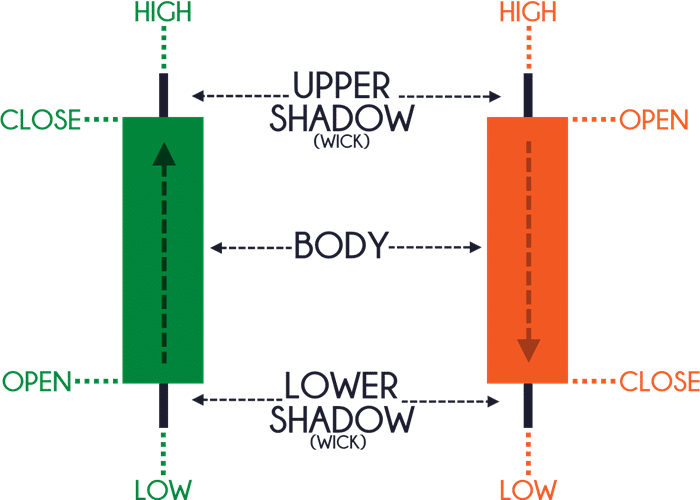
\includegraphics[width=0.4\textwidth]{Images/CandlestickChart.png}
\caption{Candlesticks showing upward (bullish) and downward (bearish) movements respectively \cite{teo_candlestick_nodate}.}
\label{Figure:CandlestickChart}
\end{figure}

This work uses tick data as its main record, because it has the finest resolution the broker provides. Whenever a coarser view is needed, it computes from the ticks the opening, highest, lowest and closing prices and the tick volume, called OHLCV data for short \cite{rhoads_candlestick_2022}. Indicators computed from that data give the model more context, as described below.

\subsection{Forex Costs: Spreads, Commissions and Overnight Financing}

Trading is not free, and its costs are large compared with the profit a single position can make. Three costs apply in Forex, and each is charged separately from the others. Prices are quoted in units that depend on the pair. A pip is the fourth decimal place of the quote for most pairs, or the second for pairs quoted against the Japanese Yen. A point is one tenth of a pip. It is the smallest price increment a broker quotes. The size of a position is given in units of the base currency, the first currency of the pair, and one standard lot is $100{,}000$ units. For a position of volume $q$ at price $p$, the notional value, which is the value of the position in the quote currency (the second currency of the pair), is

\begin{equation}
V = q \cdot p
\end{equation}

The \textbf{spread} is the first cost. It is an implicit cost, paid through the price. A position is opened at the ask and closed at the bid, so a full round trip, opening and then closing, crosses the spread once. For a position of volume $q$, the cost is

\begin{equation}
C_{spread} = (p_{ask} - p_{bid}) \cdot q
\label{Equation:SpreadCost}
\end{equation}

The spread is not constant. It widens when liquidity falls, around economic releases and at the daily rollover. A strategy tested with a fixed spread is therefore tested on a market that does not exist in practice.

The \textbf{commission} is the second cost, and it is an explicit cost. Some accounts quote the raw interbank spread. On these accounts the broker makes its money through a commission charged on the traded volume, instead of through a wider spread. If the commission is given as a number of points $c$, and $s_{point}$ is the size of one point, the cost of a position of volume $q$ is

\begin{equation}
C_{commission} = c \cdot s_{point} \cdot q
\label{Equation:CommissionCost}
\end{equation}

The spread and the commission are separate costs, and a trader pays both. On a raw-spread account, treating the spread as if it already included the commission makes trading look cheaper than it is.

The \textbf{swap}, or overnight financing, is the third cost. It comes from the interest rate differential between the two currencies of the pair. It is charged when a position is still open at the daily rollover, the moment when the trading day ends. On one day of the week the charge is multiplied, to cover the weekend. Depending on the direction of the position and the sign of the differential, the swap can be a cost or a credit. Some account types remove it completely, so that clients can avoid interest for religious reasons. These are known as swap-free accounts. Finally, leverage decides how much capital a position needs. With leverage $L$, the margin, which is the capital set aside for a position of notional value $V$, is

\begin{equation}
M = \frac{V}{L}
\end{equation}

Leverage does not change the profit or loss of a position. It only changes the capital set aside for it. So leverage affects the return of the account, and the return of the trade stays the same. These costs are not the same on every type of account. Choosing the account is therefore part of designing a strategy. A raw-spread account quotes the interbank spread with no markup and makes its money through the commission. This makes the total cost of a position lower. It also makes the cost explicit, which is more useful. The implicit part of the cost is reduced to the market spread, and the rest is a published rate. A swap-free account charges no overnight financing at all. An account with both features suits a strategy that holds positions for days. Such a strategy pays the spread and the commission only a few times per position, but it would otherwise pay financing for every night the position stays open. This work is evaluated on an account that has both features. The spread and the commission are therefore the only costs applied, and the financing cost is exactly zero, so it does not need to be estimated.

\subsection{Financial Analysis: Main Types and Formulas}

Representing the data is one half of the problem. The other half is analysing it to decide what to trade. Financial analysis is usually divided into three types \cite{lim_handbook_2015}:

\begin{itemize}
\item \textbf{Fundamental Analysis}: studies the economic factors that affect currency prices. These include GDP growth, employment rates, interest rates and monetary policy, which help to predict currency trends from the economic health of a country. However, much of this data is qualitative. This makes it hard to use in computer models, which work best with structured numerical input.
\item \textbf{Sentiment Analysis}: tries to measure the mood of the market by analysing news, market commentary and similar qualitative data. It aims to measure how the shared emotions of traders affect market trends. It is complex and needs advanced natural language processing, so it is harder to include in a model.
\item \textbf{Technical Analysis}: analyses past OHLCV data to predict future market movements. It assumes that past market behaviour will repeat itself, so patterns or measures found in current data can predict future movements. It is preferred because its results are numbers, which complex machine learning models can use.
\end{itemize}

Of the three, this work uses technical analysis. It produces numerical series directly from price data, so a model can use them without any further interpretation. Technical analysis is divided into indicators and candlestick patterns. Indicators are measures calculated from past market data, created mainly by mathematicians and economists. They give a numerical view of how the market moves. They are usually grouped into four main types \cite{lim_handbook_2015}:

\begin{itemize}
\item \textbf{Trend Indicators}: Used to find the main direction of the market by filtering out market noise. See \Cref{Tables:TrendIndicators} for details of frequently used indicators.
\item \textbf{Momentum Indicators}: Used to measure the momentum of a trend, whether it is strong or weak, and whether a reversal is expected. See \Cref{Tables:MomentumIndicators} for details of frequently used indicators.
\item \textbf{Volume Indicators}: Used to look at the trading volume, which gives clues about the strength of a price movement. See \Cref{Tables:VolumeIndicators} for details of frequently used indicators.
\item \textbf{Volatility Indicators}: Used to measure the level of uncertainty or risk that comes with the volatility of the price. See \Cref{Tables:VolatilityIndicators} for details of frequently used indicators.
\end{itemize}


The four tables list indicators in common use. They do not describe the contents of any one system. The framework built for this work implements the moving average family and the crossovers between its members, the Rate of Change, the Moving Average Convergence Divergence, the Average True Range, the Realised Volatility and the Efficiency Ratio. It implements no volume indicators. The tick volume a Forex broker reports counts quote updates, not traded size, and this limits what those indicators can measure. Ten instances of the implemented set form the observation the agent receives. They are listed in \Cref{Chapter:Implementation}. Candlestick patterns work differently. They do not compute a value. They describe shapes, formed by one or more candlesticks, that traders link to a change in behaviour \cite{rhoads_candlestick_2022}. Such patterns can be encoded as numbers and given to a model in the same way as an indicator \cite{jansen_machine_2020}. This work does not use them. The observation is built from indicators only.

\subsection{Performance Measurement: Returns, Risk and Ratios}
\label{Section:PerformanceMeasurement}

A trading strategy is judged by what it earns and by the risk it takes to earn it. A single return figure is therefore not enough to compare two strategies. The measures below are the ones reported in \Cref{Chapter:ExperimentalResults}. They are defined on an equity series, which is the value of the account over time. They therefore apply without change to a portfolio of several strategies. They are then computed on the combined equity of the portfolio, and not on each strategy separately. This matters because the risk of a portfolio depends on how its parts move together, and not only on the risk of each part.

The total return over a period compares the final and the initial equity $E$ of the account:

\begin{equation}
R = \frac{E_{final} - E_{initial}}{E_{initial}}
\end{equation}

Periods differ in length, so returns are annualised, that is, converted to a yearly rate, before they are compared. With a duration $\Delta t$ in seconds and a year of $365$ days,

\begin{equation}
R_{annual} = (1 + R)^{\frac{365 \cdot 86400}{\Delta t}} - 1
\label{Equation:AnnualizedReturn}
\end{equation}

Risk is measured in two ways. The first is volatility, which is the standard deviation of returns, annualised by the rate at which the strategy trades. The second is drawdown. At any moment, the drawdown is the distance between the current equity and the highest equity reached so far:

\begin{equation}
D(t) = \frac{E(t) - \max_{s \leq t} E(s)}{\max_{s \leq t} E(s)}
\label{Equation:Drawdown}
\end{equation}

The maximum drawdown is the worst value of $D(t)$ over the period. It is the largest loss from a peak that an investor would have suffered. The mean drawdown is the average of $D(t)$. It shows how far below its peak the account is on a typical day, instead of at its worst moment. Four ratios combine return and risk. All of them divide an annualised excess return, which is the return above the risk-free rate, by a measure of risk. They differ only in the measure of risk they use. The absolute value of that measure is used, because a drawdown is negative under the definition above. With $R_f$ as the risk-free rate,

\begin{equation}
\text{Ratio} = \frac{R_{annual} - R_f}{\left| \text{risk} \right|}
\label{Equation:RiskRatio}
\end{equation}

The \textbf{Sharpe ratio} \cite{sharpe_sharpe_1994} uses the annualised volatility, so it penalises upward and downward moves equally. The \textbf{Sortino ratio} \cite{sortino_performance_1994} uses the downside volatility instead, computed from negative returns only. The argument is that an investor does not mind upside variability. The \textbf{Calmar ratio} uses the maximum drawdown, so it measures return against the worst loss suffered. The \textbf{Sterling ratio} uses the mean drawdown. This makes it less sensitive to a single bad period, and closer to what holding the strategy is like on a typical day. The Calmar and Sterling ratios both have several definitions in the literature, and the ones used here follow \cite{bacon_practical_2023}. By construction, the mean drawdown is smaller than the maximum drawdown. So, for a strategy with a positive excess return, the Sterling ratio is the larger of the two ratios. When the excess return is negative, the order is reversed.

\subsection{Algorithmic and Quantitative Trading}

More and more of the trading in financial markets is done by algorithms. Algorithmic trading uses computer programs to execute trades faster and in larger volume than a human can. The programs analyse large datasets, read market conditions and act on set rules. Algorithmic trading is used for pre-trade analysis, signal generation and trade execution. It is what allows institutions to run complex strategies at a large scale. Quantitative trading is a subfield of algorithmic trading. It uses mathematical and statistical models to find opportunities in market data, through the analysis of past data and through machine learning. It follows systematic rules instead of the discretionary judgement of a trader, and it needs knowledge of both finance and mathematics \cite{chan_quantitative_2021}. Together, the two have changed how markets work. They brought practices such as high-frequency trading, and they shortened the time that prices take to react to new information. They have also made machine learning central to the field. Neural networks are used to find structure in market data, and reinforcement learning is used to decide what to do with it \cite{jansen_machine_2020}. These two fields are the subject of the next sections.

% !TEX root = ../../Main.tex
\section{Neural Networks}

Machine learning covers algorithms that find patterns in data and act on them, without being programmed with the rules in advance. Tom Mitchell states the idea as follows \cite{mitchell_machine_1997}:
\begin{quote}
"A computer program is said to learn from experience E with respect to some task T and some performance measure P, if its performance on T, as measured by P, improves with experience E."
\end{quote}
The definition is useful here because it describes exactly what a trading agent does. The task is choosing a position. The performance measure is the money that position makes. The experience is the market data the agent has already seen. Neural networks, the subject of this section, are the class of models used to represent that behaviour.

\subsection{Fundamentals and History}

Neural Networks (NN) are algorithms designed for pattern recognition. They are named after the human brain, because their structure is similar to it. In the brain, a neuron receives signals through structures called dendrites and processes them in the nucleus. It then passes the result down its axon to the dendrites of nearby neurons. A neural network works in a similar way. Each node is an artificial neuron. It receives an input, processes it with a mathematical function and passes the output to the next layer of nodes. In both cases, the strength and the type of the connections between neurons decide how the network behaves \cite{goodfellow_deep_2016}. \Cref{Figure:HumanNeuronVsArtificialNeuron} illustrates these ideas.

\begin{figure}[htb!]
\centering
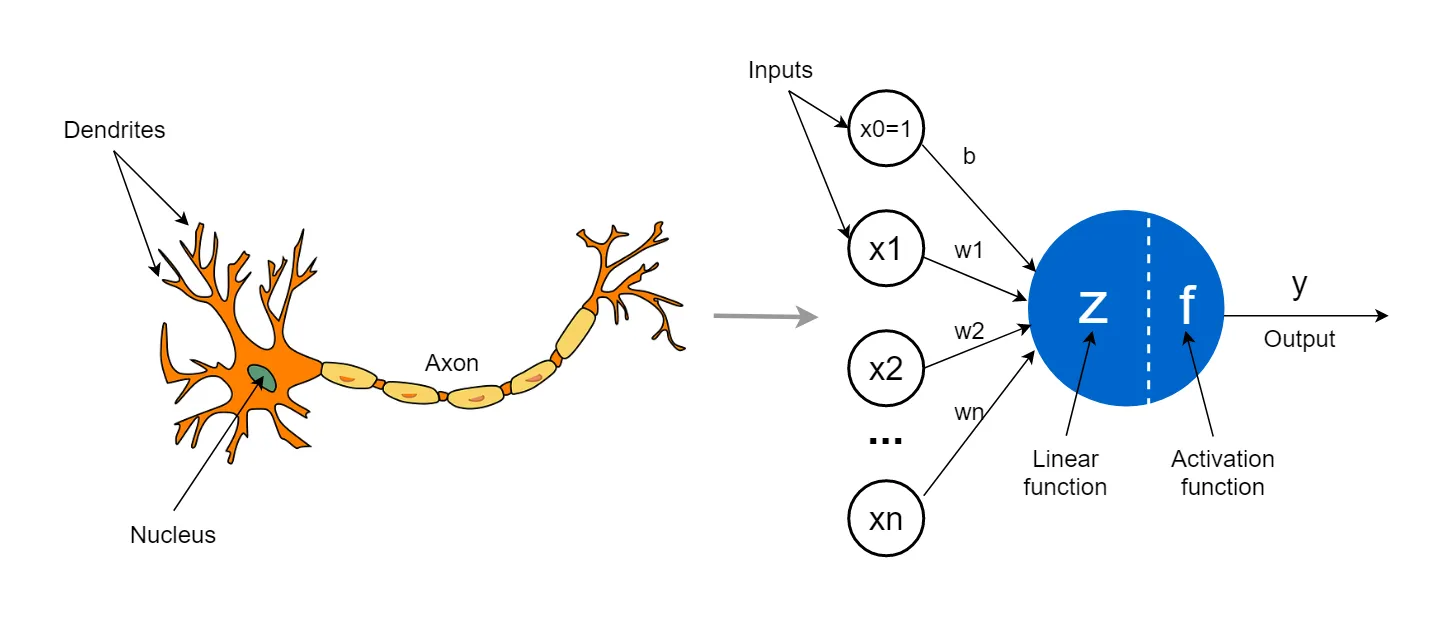
\includegraphics[width=0.7\textwidth]{Images/HumanNeuronVsArtificialNeuron.png}
\caption{Human Neuron compared to an Artificial Neuron \cite{pramoditha_human_nodate}.}
\label{Figure:HumanNeuronVsArtificialNeuron}
\end{figure}

The idea of neural networks goes back to the 1950s and the perceptron, a simple model of a biological neuron developed by Frank Rosenblatt \cite{rosenblatt_perceptron_1958}. The perceptron was the start of NN research. However, it could only learn linearly separable datasets, in which a straight line or a flat plane can separate the classes. This limit led to some periods of low interest in the field, known as ``AI winters''. A major advance came in the 1980s with the backpropagation algorithm. It allowed complex multilayer neural networks to learn patterns in datasets that are not linearly separable \cite{rumelhart_learning_1986}.

\subsection{Key Concepts and Feed-Forward}

In a neural network, the feed-forward computation in each layer \( l \) uses the output of the layer before it. For the first layer, this input \( x \) is the raw data itself. For the later layers, it is the output of the previous layer, \( h^{(l-1)}(x) \). The computation in each layer can be written as \cite{goodfellow_deep_2016}:

\begin{equation}
z^{(l)}(x) = W^{(l)} h^{(l-1)}(x) + b^{(l)}
\end{equation}

Here, the weight matrix \( W^{(l)} \in \mathbb{R}^{K_l \times K_{l-1}} \) and the bias vector \( b^{(l)} \in \mathbb{R}^{K_l} \) are used in the computation of layer \( l \). \( K_l \) is the number of neurons, or units, in layer \( l \), and \( K_{l-1} \) is the number of neurons in the previous layer \( l-1 \). For the first layer, \( W^{(1)} \in \mathbb{R}^{K_1 \times D} \), where \( D \) is the size of the input data. The activation function \( g \) is then applied to the pre-activation \( z^{(l)}(x) \in \mathbb{R}^{K_l} \) to give the activated output \( h^{(l)}(x) \in \mathbb{R}^{K_l} \) \cite{goodfellow_deep_2016}:

\begin{equation}
h^{(l)}(x) = g(z^{(l)}(x))
\end{equation}

The choice of activation function matters in two places. In the hidden layers, the function must be non-linear. A stack of linear layers is equal to a single linear transformation, so the network would gain nothing from its depth. In the output layer, the task decides the function. A bounded function is used when the output must stay within a range, and no activation is used when it does not \cite{goodfellow_deep_2016}. \Cref{Tables:ActivationFunctions} summarises the most common activation functions.

% !TEX root = ../Main.tex
\begin{table}[htb!]
\centering
\footnotesize
\caption{Summary of the most common Activation Functions \cite{goodfellow_deep_2016}.}
\label{Tables:ActivationFunctions}
\begin{tabularx}{\textwidth}{@{}lXl@{}}
\toprule
\textbf{Activation Function} & \textbf{Formula} & \textbf{Description} \\
\midrule
Linear & \( a(x) = x \) & Suitable for regression tasks. \\
\addlinespace
Sigmoid & \( \sigma(x) = \frac{1}{1 + e^{-x}} \) & Maps inputs to (0, 1), for binary classification. \\
\addlinespace
Hyperbolic Tangent & \( \tanh(x) = \frac{e^{x} - e^{-x}}{e^{x} + e^{-x}} \) & Maps inputs to (-1, 1), with stronger gradients than sigmoid. \\
\addlinespace
ReLU & \( \text{ReLU}(x) = \max(0, x) \) & Leads to sparse activation, helps gradient flow. \\
\addlinespace
Softmax & \( \text{Softmax}(z)_i = \frac{e^{z_i}}{\sum_{k=1}^K e^{z_k}} \) & Turns raw scores (logits) into probabilities, for multi-class classification. \\
\bottomrule
\end{tabularx}
\end{table}

\subsection{Learning using Backpropagation}

Neural networks learn by adjusting their weights and biases step by step, to reduce the error between the predicted outputs and the true target values. A loss function measures this error and guides the learning. The goal is to find the parameters that minimise the loss function. Different problems need different loss functions, such as mean squared error for regression tasks and cross-entropy for classification \cite{goodfellow_deep_2016}. \Cref{Tables:LossFunctions} gives their formulas.

% !TEX root = ../Main.tex
\begin{table}[htb!]
\centering
\footnotesize
\caption{Summary of the most common Loss Functions \cite{goodfellow_deep_2016}.}
\label{Tables:LossFunctions}
\begin{tabularx}{\textwidth}{@{}lXl@{}}
\toprule
\textbf{Loss Function} & \textbf{Formula} & \textbf{Application} \\
\midrule
Mean Squared Error (MSE) & \( \frac{1}{n} \sum_{i=1}^n (y_i - \hat{y}_i)^2 \) & Regression \\
\addlinespace
Negative Log-Likelihood (Cross-Entropy) & \( -\sum_{i=1}^n y_i \log(\hat{y}_i) \) & Classification \\
\bottomrule
\end{tabularx}
\end{table}

The main algorithm used to train neural networks is called backpropagation \cite{rumelhart_learning_1986}. It computes the gradient of the loss function with respect to the weights and biases of the network. The gradient points in the direction of steepest increase of the loss. \Cref{Codes:GradientLossFunction} shows how these gradients are calculated. Gradient descent then moves the weights and biases in the opposite direction, which reduces the loss. Its variants, listed with their formulas in \Cref{Tables:GradientDescent}, suit different data and computing needs. Batch gradient descent uses the whole dataset for each update. It is stable but expensive on large datasets. Stochastic gradient descent updates the parameters after every data point. It is faster but noisier. Mini-batch gradient descent updates on subsets of the data. It is the compromise used in practice \cite{goodfellow_deep_2016}.

% !TEX root = ../Main.tex
\begin{algorithm}[htb!]
\DontPrintSemicolon
\KwRequire{\( f \): network function, \( \theta \): network parameters, \( x \): input data, \( y \): true label, \( l \): number of layers, \( L \): loss function}
Compute the output of the network \( \hat{y} = f(x; \theta) \)\;
Compute the gradient of the loss function with respect to the output layer before activation:\;
\( \nabla_{z^{(l+1)}}L(f(x; \theta), y) = \frac{\partial L(f(x; \theta), y)}{\partial \hat{y}} \cdot \frac{\partial \hat{y}}{\partial z^{(l+1)}} \)\;
\For{\( \ell = l+1 \) to \( 1 \)}{
    Compute gradients of hidden layer parameters:\;
    \( \nabla_{W^{(\ell)}}L(f(x; \theta), y) = \nabla_{z^{(\ell)}}L(f(x; \theta), y) \cdot h^{(\ell-1)T} \)\;
    \( \nabla_{b^{(\ell)}}L(f(x; \theta), y) = \nabla_{z^{(\ell)}}L(f(x; \theta), y) \)\;
    Compute gradient of previous hidden layer:\;
    \( \nabla_{h^{(\ell-1)}}L(f(x; \theta), y) = W^{(\ell)T} \cdot \nabla_{z^{(\ell)}}L(f(x; \theta), y) \)\;
    Compute gradient of previous hidden layer (before activation):\;
    \( \nabla_{z^{(\ell-1)}}L(f(x; \theta), y) = \nabla_{h^{(\ell-1)}}L(f(x; \theta), y) \odot g'(z^{(\ell-1)}) \)\;
}
\caption{Gradient of the Loss Function \cite{goodfellow_deep_2016}.}
\label{Codes:GradientLossFunction}
\end{algorithm}

In \Cref{Tables:GradientDescent}, the learning rate \( \eta \) is a hyperparameter that controls the size of each update. A rate that is too large overshoots the minimum. A rate that is too small converges slowly and can get stuck in a local minimum. Some methods adapt \( \eta \) during training. They change the step size as the optimisation goes on, and this deals with both problems. Normalising or standardising the input data has the same aim, because features on very different scales produce gradients on very different scales \cite{goodfellow_deep_2016}.

% !TEX root = ../Main.tex
\begin{table}[htb!]
\centering
\footnotesize
\caption{Summary of the most common Gradient Descent variants \cite{goodfellow_deep_2016}.}
\label{Tables:GradientDescent}
\begin{tabularx}{\textwidth}{@{}lXl@{}}
\toprule
\textbf{Algorithm} & \textbf{Formula} & \textbf{Description} \\
\midrule
Batch Gradient Descent & \(\theta := \theta - \eta \cdot \nabla_{\theta} J(\theta; X, y)\) & Updates the parameters using all the data \\
\addlinespace
Mini-Batch Gradient Descent & \(\theta := \theta - \eta \cdot \nabla_{\theta} J(\theta; X^{(i:i+n)}, y^{(i:i+n)})\) & Updates the parameters using subsets of the data \\
\addlinespace
Stochastic Gradient Descent & \(\theta := \theta - \eta \cdot \nabla_{\theta} J(\theta; x^{(i)}, y^{(i)})\) & Updates the parameters after each data point \\
\bottomrule
\end{tabularx}
\end{table}

\subsection{Bias-Variance Trade-off and Model Generalisation}

How well a neural network generalises, that is, how well it works on data it has not seen, depends on a balance between bias and variance. Bias leads to underfitting. The model makes assumptions that are too simple and misses the real trends in the data. Variance leads to overfitting. The model is too complex and treats noise as if it were a signal. Both give poor results on new data. This matters in Forex trading, because the signal being sought is weak and the noise around it is large. Cross-validation is often used to measure how well a model generalises, on separate training, validation and testing datasets. Regularisation methods such as L1 and L2 limit the complexity of a model by adding penalties to the loss function. Dimensionality reduction methods such as principal component analysis reduce the number of inputs the model has to fit. Together, these methods make it more likely that the model performs well on out-of-sample data, which is data not used in training \cite{goodfellow_deep_2016}. This work divides the period into training, validation and testing windows, described in \Cref{Chapter:Implementation}. The performance on the validation window decides which model is kept. Complexity is not controlled through a penalty added to the loss.

\subsection{Architectures for Sequential Data}

The network described so far is feed-forward. The whole input is given at once, and the output depends only on that input. Financial data is a sequence, so an obvious question is whether a network that reads a sequence directly would do better.

Two families of networks do that. A recurrent neural network keeps an internal state that is carried from one step to the next, so each observation is read together with the ones before it. The long short-term memory network is the variant used in practice. It adds gates that control what the state keeps and what it drops. This stops the gradient from vanishing, that is, from shrinking towards zero, as it is propagated back over many steps \cite{goodfellow_deep_2016}. Attention-based networks reach the same goal in a different way. They let the network weigh every position in a window directly, instead of passing information along a chain.

Much of the work reviewed in \Cref{Chapter:RelatedWork} uses recurrent networks, and several of those studies report that they helped. This work does not use them, and this was a deliberate design decision. Recurrence is one way to give a network access to the past. Another way is to compute measures of the past explicitly and give them to the network as part of the input. The observation described in \Cref{Chapter:Implementation} uses the second way. It includes momentum and moving-average readings over horizons from one day to one year. The history that a recurrent state would have to learn to summarise is therefore measured directly and given to the network.

This choice has three consequences. First, a feed-forward network on engineered features has far fewer parameters than a recurrent network on raw prices. This matters when the signal is weak and the sample is one instrument over eleven years. Second, it is faster to train. Training speed decided how many independent runs were possible, and this turned out to matter more for the quality of the final result than any gain from a different architecture would have. Third, it keeps the input interpretable. Each feature is a named quantity with a known meaning, so when a policy behaves strangely, the observation can be inspected instead of guessed at.

This choice also has a cost. A recurrent network can, in principle, find a summary of the past that no fixed set of indicators contains. This work gives up that possibility. Whether it would have helped here has not been tested, and it is listed among the extensions in \Cref{Section:FutureWork}.

\subsection{Universal Approximation Theorem}

The universal approximation theorem, proved by Hornik, Stinchcombe and White in 1989, can be stated as follows \cite{hornik_multilayer_1989}:

\begin{quote}
A neural network with one hidden layer and a linear output can approximate any continuous function arbitrarily well, given enough hidden units.
\end{quote}

The theorem shows that neural networks are universal function approximators, and this is what justifies their use here. It means that a large enough network can represent the function that maps market observations to a trading decision. It does not say whether such a function can be found from data, or whether it exists in a form stable enough to be useful. Those questions are the subject of the reinforcement learning methods covered next.

% !TEX root = ../../Main.tex
\section{Reinforcement Learning}
\label{Section:ReinforcementLearning}

Reinforcement Learning (RL) is the branch of machine learning that studies an agent that interacts with an environment and learns which decisions to make. Unlike supervised learning, it is not given the correct answer for any situation. The agent acts, observes what happens and changes its behaviour according to the reward it receives. Learning therefore happens by trial and error, without labelled examples. This suits problems where the right action is not known in advance but its outcome can be measured. Robotics and finance are two fields where this is the case.

\subsection{Fundamentals and History}

Reinforcement Learning grew out of the combination of several other fields, such as psychology, computer science and control theory. It was inspired by the way humans and animals learn from their environment. In RL, an agent makes decisions and receives rewards or penalties for its actions, with the aim of maximising good outcomes over time. This process is based on operant conditioning, a type of learning studied by psychologists such as B. F. Skinner \cite{skinner_operant_1963}, in which behaviour is shaped by its consequences. Markov Decision Processes (MDPs) were formalised in the late 1950s. They model decision making where the outcomes are partly random and partly under the control of the decision maker. MDPs became the mathematical basis of RL, because they allowed the development of algorithms that learn optimal strategies in complex environments. One of the major advances in RL was Q-Learning, introduced in the late 1980s. It is an algorithm that learns the value of actions in different states, so an agent can make informed decisions without a model of the environment. Q-Learning and Temporal Difference Learning made it possible to apply RL to a wide range of problems, from playing video games better than humans to optimising financial trading strategies \cite{sutton_reinforcement_2018}.

\subsection{Key Concepts and Agent-Environment Interaction}

Reinforcement Learning is about how an agent interacts with its environment. The interaction involves states, actions and rewards. The state \( S_t \) describes the situation of the agent at that moment. When the agent observes \( S_t \), it chooses an action \( A_t \). This action makes the environment transition to a new state \( S_{t+1} \), and the environment gives feedback in the form of a reward \( R_{t+1} \). \Cref{Figure:AgentEnvironment} shows this repeating cycle \cite{sutton_reinforcement_2018}.

\begin{figure}[htb!]
\centering
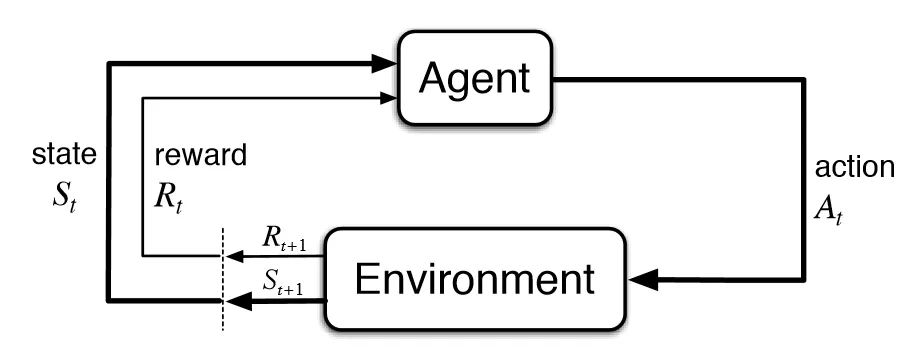
\includegraphics[width=0.6\textwidth]{Images/AgentEnvironment.png}
\caption{Interaction between the agent and the environment in Reinforcement Learning \cite{sutton_reinforcement_2018}.}
\label{Figure:AgentEnvironment}
\end{figure}

The goal of the agent is to maximise the return. The return is the discounted sum of the rewards the agent collects from time \( t \) onwards \cite{sutton_reinforcement_2018}:

\begin{equation}
R_{t+1} + \gamma R_{t+2} + \gamma^2 R_{t+3} + \ldots = \sum_{k=0}^{\infty} \gamma^k R_{t+k+1}
\end{equation}

Here, \( \gamma \) is the discount factor. It sets how much future rewards count compared with immediate ones. A policy \( \pi \) decides the actions of the agent. It can be deterministic, giving one specific action for each state, or stochastic, giving a probability distribution over actions. A main difficulty in RL is the balance between exploration and exploitation. Exploration means trying new actions to find out their effects. Exploitation means choosing actions that are known to give a high reward. A common approach is the \(\varepsilon\)-greedy policy, which usually picks the best-known action but sometimes picks a random one \cite{sutton_reinforcement_2018}. This method needs a discrete set of actions, because it works by picking one of the alternatives at random. When the action is continuous, as in this work, exploration comes instead from adding noise to the action the policy returns. \Cref{Section:DeepReinforcementLearning} describes this approach together with the algorithm that uses it.

Reinforcement Learning is built on the Markov Decision Process (MDP), defined by the tuple \( (S, A, P, R, \gamma) \). Here, \( S \) is the set of all possible states of the environment and \( A \) is the set of actions the agent can take. \( P \) is the transition probability, the probability of moving from state \( s_t \) to state \( s_{t+1} \) after taking action \( a \). \( R \) is the reward function, which gives the reward for that transition, and \( \gamma \) is the discount factor. MDPs rely on the Markov property. It requires the next state to depend only on the current state and action, and not on any earlier ones \cite{sutton_reinforcement_2018}:

\begin{equation}
\label{Equation:MarkovProperty}
P(s_{t+1} | s_t, a_t, s_{t-1}, a_{t-1}, \ldots, s_0, a_0) = P(s_{t+1} | s_t, a_t)
\end{equation}

The reward function matters because it is where the goal of the task is defined. It tells the agent what to achieve, but not how to achieve it. The agent will adopt any behaviour that raises the reward. In trading, the reward is normally computed from profit and loss. This drives the agent towards profitable positions without telling it which positions those are \cite{sutton_reinforcement_2018}.

\subsection{Value Functions and Q-Functions}

The value function of a policy \( \pi \), written \( V^\pi(s) \), is the expected return when starting in state \( s \) and following policy \( \pi \) after that. It is defined as follows \cite{sutton_reinforcement_2018}:

\begin{equation}
V^\pi(s) = \mathbb{E} \left[ \sum_{k=0}^{\infty} \gamma^k R_{t+k+1} \mid S_t = s, \pi \right]
\end{equation}

Here, \( \gamma \) is the discount factor, which sets how much future rewards count compared with immediate rewards. \( \mathbb{E} \) is the expected value, the average of all possible outcomes weighted by their probabilities. The Q-function of a policy \( \pi \), written \( Q^\pi(s, a) \), is the expected return for taking action \( a \) in state \( s \) and following policy \( \pi \) after that. It is defined as follows \cite{sutton_reinforcement_2018}:

\begin{equation}
Q^\pi(s, a) = \mathbb{E} \left[ \sum_{k=0}^{\infty} \gamma^k R_{t+k+1} \mid S_t = s, A_t = a, \pi \right]
\end{equation}

The Bellman equations are named after Richard Bellman, who first formulated them. They give a recursive decomposition of the total cumulative reward an agent can expect, starting from a given state or state-action pair. These equations are the basis of dynamic programming methods in RL. They express the value of a state, or of a state-action pair, in terms of the values of the states that follow it. This recursion is what allows the estimated values to be improved step by step, and it is the basis of convergence for most RL algorithms. The equations are as follows \cite{sutton_reinforcement_2018}:

\begin{equation}
V^\pi(s) = \sum_{a \in A} \pi(a|s) \sum_{s' \in S} P(s'|s,a) \left[ R(s,a,s') + \gamma V^\pi(s') \right]
\end{equation}

\begin{equation}
Q^\pi(s, a) = \sum_{s' \in S} P(s'|s,a) \left[ R(s,a,s') + \gamma \sum_{a' \in A} \pi(a'|s') Q^\pi(s', a') \right]
\end{equation}

\begin{equation}
\label{Equation:RelationshipValueQFunction}
V^\pi(s) = \sum_{a \in A} \pi(a|s) Q^\pi(s, a)
\end{equation}

\Cref{Equation:RelationshipValueQFunction} shows that the value of a state under policy \(\pi\) is the expected value of the Q-function over all possible actions, weighted by the probability the policy gives to each action. For optimal policies, the optimal value function \( V^*(s) \) and the optimal Q-function \( Q^*(s, a) \) give the highest return that can be achieved from any state or state-action pair, respectively. From the Bellman equation, it follows that \cite{sutton_reinforcement_2018}:

\begin{equation}
V^*(s) = \max_{a \in A} \sum_{s' \in S} P(s'|s,a) \left[ R(s,a,s') + \gamma V^*(s') \right]
\end{equation}

\begin{equation}
Q^*(s, a) = \sum_{s' \in S} P(s'|s,a) \left[ R(s,a,s') + \gamma \max_{a' \in A} Q^*(s', a') \right]
\end{equation}

\begin{equation}
V^*(s) = \max_{a \in A} Q^*(s, a)
\end{equation}

By applying these equations again and again, RL algorithms gradually approximate the value function and the Q-function. This guides the agent towards the optimal policy, which is the policy that maximises the expected cumulative reward \cite{sutton_reinforcement_2018}.

\subsection{Methodological Variants and Learning Methods}

Reinforcement learning methods can be divided into groups by the properties of the learning method: model-based or model-free, on-policy or off-policy, and value-based or policy-based. In model-based RL, the algorithm builds a model of the environment to simulate and predict the outcomes of actions. The agent can then plan by predicting the next states. This is possible when the environment is simple enough to be modelled. In model-free RL, the algorithm learns a policy or a value function directly from its interactions with the environment, without building a model of it. Model-free methods are often chosen when the environment is hard to model or when no accurate model is available. Within model-free RL, there are on-policy methods, which learn about the policy that is currently used to make decisions, and off-policy methods, which explore with a different policy while they try to learn an optimal one \cite{sutton_reinforcement_2018}.

Another important distinction is between value-based methods, also called critic-only, and policy-based methods, also called actor-only. Value-based methods, such as Temporal Difference Learning (TD), Q-Learning and SARSA Learning, estimate the value of states or of state-action pairs. The policy is not learned directly. It follows from these values. Temporal Difference learning is the update rule that the other two are built on, and it works in both settings. SARSA is on-policy, because it evaluates the policy it is following. Q-Learning is off-policy, because it evaluates the greedy policy, the one that always takes the highest-valued action, whatever policy it actually follows. To take the highest-valued action, the method has to compare every action, so these methods are limited to discrete sets of actions. Policy-based methods, such as REINFORCE, optimise the policy directly. For this reason they extend to continuous actions, where the policy returns the action itself instead of a value for each possible action. Actor-Critic learning combines the two. It has a policy function (the actor) and a value function (the critic). The policy is improved directly, and the critic gives the value estimates that make those updates stable \cite{sutton_reinforcement_2018}. \Cref{Codes:ActorCritic} gives a detailed implementation.

% !TEX root = ../Main.tex
\begin{algorithm}[htb!]
\DontPrintSemicolon
\KwRequire{$\pi(a \mid s; \theta)$: a differentiable policy, $Q(s, a; w)$: a differentiable $Q$-function, $N$: number of iterations and learning rates $\beta^\theta > 0$ and $\beta^w > 0$}
Initialise policy parameter $\theta^{(0)}$ and $Q$-function parameter $w^{(0)}$\;
Initialise state $s$\;
\For{$n = 0, 1, \ldots, N - 1$}{
    Sample $a \sim \pi(\cdot \mid s; \theta^{(n)})$\;
    Take action $a$, observe state $s'$ and reward $r$\;
    Sample $a' \sim \pi(\cdot \mid s'; \theta^{(n)})$\;
    Compute the TD error: $\delta \gets r + \gamma Q(s', a'; w^{(n)}) - Q(s, a; w^{(n)})$\;
    Update $w$: $w^{(n+1)} \gets w^{(n)} + \beta^w \delta \nabla_w Q(s, a; w^{(n)})$\;
    Update $\theta$: $\theta^{(n+1)} \gets \theta^{(n)} + \beta^\theta \delta \nabla_\theta \ln \pi(a \mid s; \theta^{(n)})$\;
    $s \gets s'$\;
}
\caption{Actor-Critic \cite{sutton_reinforcement_2018}.}
\label{Codes:ActorCritic}
\end{algorithm}

For finite Markov Decision Processes, standard results guarantee that an optimal policy exists and that it can be taken to be deterministic and stationary. These guarantees do not extend to complex, non-stationary environments such as financial markets \cite{sutton_reinforcement_2018}. A raw price series does not have the Markov property. The information a trader uses is spread across the recent history, and is not all contained in the latest quote. RL applied to these markets therefore works with an approximation. Technical indicators and other engineered features put enough of that history into the state for the Markov property to hold approximately. Actor-Critic methods matter here because they are the point where reinforcement learning and neural networks meet. This is the subject of the next section.

% !TEX root = ../../Main.tex
\section{Deep Reinforcement Learning}
\label{Section:DeepReinforcementLearning}

Deep Reinforcement Learning (DRL) combines the decision making of reinforcement learning with the function approximation of neural networks. The value functions and policies of \Cref{Section:ReinforcementLearning} are defined over states. In a tabular setting, each state is stored separately, as one entry in a table. This is not possible when the state is a vector of continuous market variables, because there is no limit to the number of distinct states. Replacing the table with a neural network removes that limit. It also lets the agent generalise from states it has seen to states it has not seen.

\subsection{Fundamentals and History}

DRL appeared once it became clear that neural networks could serve as the function approximators that reinforcement learning needed to handle high-dimensional input. The result that started the field was the Deep Q-Network. It learned to play a range of Atari 2600 games directly from raw pixels and reached human-level scores on many of them \cite{mnih_playing_2013, mnih_human-level_2015}. It showed that a single architecture could learn control policies from raw, high-dimensional input, without features designed for each task. This result led to interest in applying the same methods to financial markets. There, the input is also high-dimensional, and the mapping from observation to decision is also unknown. However, an Atari game is stationary and fully observable, and a market is neither. For this reason, results carry over to markets much less directly than the comparison with games suggests.

\subsection{Deep Value-Based RL Algorithms: Deep Q-Networks}

Deep value-based methods use a neural network to approximate the Q-function. This lets them work with state spaces too large to list one by one. Neural Fitted Q Iteration was an early method of this kind. It fitted a network to the Q-values of a stored set of transitions, and fitted it again as more transitions were collected \cite{riedmiller_neural_2005}. The approach became established with the Deep Q-Network (DQN) algorithm \cite{mnih_human-level_2015}, which added two mechanisms that made training stable enough to be practical. The first is a separate target network. This is a delayed copy of the value network, used to compute the learning targets, so that the target does not move as fast as the estimate. The second is experience replay. This is a buffer of past transitions from which mini-batches are drawn at random, which breaks the temporal correlation between consecutive samples. The algorithm used in this work uses both mechanisms.

After DQN, the Double Deep Q-Network (DDQN) dealt with the tendency of DQN to overestimate action values \cite{van_hasselt_deep_2016}. It separates action selection from action evaluation. The online network, the one being trained, chooses the action, and the target network scores it. Deep value-based methods are not used in this work. They select an action by comparing the values of all available actions, and this requires the set of actions to be discrete.

\subsection{Deep Policy-Based RL Algorithms: Deep Policy Gradients}

Deep policy-based algorithms optimise the policy directly, without deriving it from action values. This is what allows them to work with continuous actions. In trading this matters, because a position has a size as well as a direction. A method limited to a discrete set of actions has to decide that size outside the learned policy. The Deep Deterministic Policy Gradient (DDPG) algorithm is a model-free, off-policy, actor-critic method for continuous action spaces \cite{lillicrap_continuous_2015}. It keeps four networks. The actor \( \mu(s | \theta^{\mu}) \) maps a state to a single action. The critic \( Q(s, a | \theta^{Q}) \) estimates the value of a state-action pair. The other two are delayed copies of these, the target actor \( \mu' \) and the target critic \( Q' \). Transitions are stored in a replay buffer, and mini-batches of \( N \) transitions are sampled from it at random. The critic is trained in the same way as in DQN. It minimises the squared error between its estimate and a target built from the observed reward and the value of the next state \cite{lillicrap_continuous_2015}:

\begin{equation}
y_i = r_i + \gamma \, Q'\!\left(s_{i+1}, \mu'(s_{i+1} | \theta^{\mu'}) \,\middle|\, \theta^{Q'}\right)
\label{Equation:DDPGTarget}
\end{equation}

\begin{equation}
L = \frac{1}{N} \sum_{i} \left( y_i - Q(s_i, a_i | \theta^{Q}) \right)^2
\label{Equation:DDPGCriticLoss}
\end{equation}

The actor is updated with the deterministic policy gradient, which follows the direction in which the value estimated by the critic increases. Because the action is continuous, the gradient of the value with respect to the action is defined, and the chain rule carries it back to the parameters of the actor \cite{lillicrap_continuous_2015}:

\begin{equation}
\nabla_{\theta^{\mu}} J \approx \frac{1}{N} \sum_{i} \nabla_{a} Q(s, a | \theta^{Q}) \big|_{s = s_i,\, a = \mu(s_i)} \; \nabla_{\theta^{\mu}} \mu(s | \theta^{\mu}) \big|_{s_i}
\label{Equation:DeterministicPolicyGradient}
\end{equation}

The target networks are not simply copied from the trained networks. After every update, they are moved a small fraction \( \tau \ll 1 \) towards them. This keeps the learning targets almost stationary, but it also slows down how fast they follow improvements \cite{lillicrap_continuous_2015}:

\begin{equation}
\theta' \leftarrow \tau \theta + (1 - \tau) \theta'
\label{Equation:SoftUpdate}
\end{equation}

The policy is deterministic, so it does not explore by itself, and the exploration problem raised in \Cref{Section:ReinforcementLearning} comes back here. DDPG solves it by adding a noise process \( \mathcal{N} \) to the action during training, so the action actually executed is \( \mu(s | \theta^{\mu}) + \mathcal{N} \). The original work uses an Ornstein-Uhlenbeck process. This process gives noise that is correlated in time, instead of independent at each step. The reason given is that a physical system with momentum explores better when a disturbance lasts for a while than when it changes sign at every step \cite{lillicrap_continuous_2015}. \Cref{Codes:DeepDeterministicPolicyGradient} shows the complete procedure.

% !TEX root = ../Main.tex
\begin{algorithm}[htb!]
\DontPrintSemicolon
\KwRequire{an actor $\mu(s | \theta^{\mu})$, a critic $Q(s, a | \theta^{Q})$, a discount factor $\gamma$, a soft update rate $\tau \ll 1$ and a minibatch size $N$}
Randomly initialise the critic parameters $\theta^{Q}$ and the actor parameters $\theta^{\mu}$\;
Initialise the target parameters $\theta^{Q'} \leftarrow \theta^{Q}$ and $\theta^{\mu'} \leftarrow \theta^{\mu}$, and the replay buffer $\mathcal{B}$\;
\For{episode $= 1, M$}{
    Initialise a random process $\mathcal{N}$ for action exploration\;
    Receive the initial observation state $s_1$\;
    \For{$t = 1, T$}{
        Select the action $a_t = \mu(s_t | \theta^{\mu}) + \mathcal{N}_t$ from the current policy and the exploration noise\;
        Execute the action $a_t$ and observe the reward $r_t$ and the new state $s_{t+1}$\;
        Store the transition $(s_t, a_t, r_t, s_{t+1})$ in $\mathcal{B}$\;
        Sample a random minibatch of $N$ transitions $(s_i, a_i, r_i, s_{i+1})$ from $\mathcal{B}$\;
        Set $y_i = r_i + \gamma Q'(s_{i+1}, \mu'(s_{i+1} | \theta^{\mu'}) | \theta^{Q'})$\;
        Update the critic by minimising the loss: $L = \frac{1}{N}\sum_i (y_i - Q(s_i, a_i | \theta^{Q}))^2$\;
        Update the actor policy using the sampled policy gradient:\;
        $\nabla_{\theta^{\mu}} J \approx \frac{1}{N}\sum_i \nabla_a Q(s, a | \theta^{Q})|_{s = s_i, a = \mu(s_i)} \nabla_{\theta^{\mu}} \mu(s | \theta^{\mu})|_{s_i}$\;
        Update the target networks:\;
        $\theta^{Q'} \leftarrow \tau \theta^{Q} + (1 - \tau) \theta^{Q'}$\;
        $\theta^{\mu'} \leftarrow \tau \theta^{\mu} + (1 - \tau) \theta^{\mu'}$\;
    }
}
\caption{Deep Deterministic Policy Gradient \cite{lillicrap_continuous_2015}.}
\label{Codes:DeepDeterministicPolicyGradient}
\end{algorithm}

DDPG is powerful, but it is not reliable. It has no guarantee of convergence except under restrictive conditions. It is also known to be sensitive to its hyperparameters and to the random seed, so two runs of the same configuration can end with different policies. A market makes this worse. It is non-stationary and only partially observable, which means the agent does not see the full state, and the guarantees that apply to finite Markov Decision Processes do not hold. These limits belong to the method itself. They are not problems that can be fixed. \Cref{Chapter:ExperimentalResults} therefore reports how the results vary, instead of reporting a single run.

This work combines the four topics covered here. It needs a market to trade in, networks to approximate the functions involved, a reinforcement learning formulation of the trading decision, and an algorithm that solves it for continuous actions. Combining them is not new. Many published studies have already tried it.

Those studies differ in how they define the state, the action and the reward. They also differ in whether the agent pays any cost for trading. These choices decide whether a reported result would hold on a live account. This makes them the right basis for comparing the published studies and for placing this work among them.
\cleardoublepage
%
% !TEX root = ../../Main.tex
\fancychapter{Related Work}
\label{Chapter:RelatedWork}

This chapter reviews the published work on deep reinforcement learning for financial trading. The review had two stages. First, surveys were read to find which problems the field still sees as open and which papers are worth reading in full. Then single articles were read, and their design choices were recorded in one common format. This way, studies that use different markets and different algorithms could be compared on the same points.

Eighteen articles were read in this way. \Cref{Tables:BasicRelatedWork} lists their basic features, and \Cref{Tables:AdvancedRelatedWork} lists the design choices inside each agent. The text below refers to both tables.

% !TEX root = ../../Main.tex
\section{Survey Research: Identifying the State-of-the-Art}

The review started with surveys. A survey shows the main lines of a field faster than single papers do, and it points back to the work that first showed each result.

Hambly et al. \cite{hambly_recent_2023} gave the theoretical basis. The survey first explains reinforcement learning and neural networks on their own. It then covers how the two combine into deep reinforcement learning, and how this has been applied in finance. It gives the mathematical formulations and pseudocode for critic-only, actor-only and actor-critic algorithms, together with the papers that introduced each of them. It is the reference that was used to write \Cref{Chapter:Background}.

Fischer \cite{fischer_reinforcement_2018} had the opposite purpose. It is about practice, not theory, and it reviews implementations, not derivations. This work took from it the list of dimensions it uses to compare studies: the dataset, the network under the reinforcement learning agent, the state space, the action space, the reward function, the methods used for the bias-variance and exploration-exploitation trade-offs, and the training procedure. These dimensions became the columns of \Cref{Tables:BasicRelatedWork} and \Cref{Tables:AdvancedRelatedWork}. In this way the articles below could all be compared on the same points, and not only described one at a time.

Three more surveys were also read \cite{pricope_deep_2021, alameer_reinforcement_2022, meng_reinforcement_2019}. They agree on the general picture. Most work in the field uses equity markets, daily data and discrete trading decisions. Reported results are hard to compare, because the trading environment is different in each paper.

% !TEX root = ../../Main.tex
\section{Article Research: Summarising Different Implementations}

Next, eighteen articles with working implementations were read in full. Their features were recorded in two tables that cover the same articles. \Cref{Tables:BasicRelatedWork} holds the market, the data and the algorithm used. \Cref{Tables:AdvancedRelatedWork} holds the design choices inside each agent. Below, the articles are grouped by the market they trade.


\subsection{Forex Market Implementations}

Three of the eighteen articles trade currencies. All three limit the agent to a discrete choice between buying, holding and selling.

Carapuço et al. \cite{carapuco_reinforcement_2018} built a Deep Q-Network over a fully connected network and used it on raw tick data from 2010 to 2017. The agent could act only after a fixed number of ticks had passed. This gave about one decision every two hours. It outperformed its benchmark by a wide margin. It is also the only study reviewed here that works from tick data and not from bars. Huang \cite{huang_financial_2018} used a Deep Recurrent Q-Network on 15-minute bars from 2012 to 2017. This model puts a long short-term memory network under the Q-function. It outperformed its benchmark with explicit and implicit trading costs charged. This makes it one of the few results in the set that still hold when costs are modelled. Rundo \cite{rundo_deep_2019} used the same kind of model on one-minute bars from 2004 to 2018, and also reported that it outperformed its benchmark. However, its accuracy was high enough to suggest look-ahead bias, and its maximum drawdown was large. Taken together, the two results suggest that adding recurrence is not enough on its own to make very short timeframes workable.

\subsection{Stock Market Implementations}

Most of the work reviewed trades in equity markets. Among the critic-only studies, Sim and Kirk \cite{sim_generalized_2023} trained a Deep Q-Network on daily bars from 2006 to 2022. They tested it on assets it had not seen, and reported that the policy generalised to them. Théate and Ernst \cite{theate_application_2021} used the same algorithm on daily bars from 2012 to 2019. They reported consistent results in both calm and volatile periods. Their agent explored through an inverted copy of the environment, instead of through a noise process. Li et al. \cite{li_deep_2019} compared two agents on minute bars of stocks and futures from 2010 to 2020. The first was a Deep Q-Network over a denoising autoencoder. The second was Asynchronous Advantage Actor Critic over a long short-term memory network. Both beat the benchmark. The asynchronous actor-critic converged better, and the authors attribute this to its parallel training.

The actor-critic studies are closer to the design used in this work. Xiong et al. \cite{xiong_practical_2018} applied DDPG to daily bars from 2009 to 2018 and outperformed the benchmark. Yousefi \cite{yousefi_deep_2022} compared DDPG with Advantage Actor Critic on daily bars from 2009 to 2021. DDPG was the more stable of the two, and the study attributes this to its replay buffer and its noise process. Gran et al. \cite{gran_deep_2019} ran DDPG on monthly bars from 2005 to 2019. It still outperformed the benchmark after explicit and implicit costs were charged. Azhikodan et al. \cite{saini_stock_2019} added news sentiment to a state space that already held price data and technical indicators. They reported that this improved the results. However, the evaluation covers about five months, and the exact period is not given. Majidi et al. \cite{majidi_algorithmic_2022} used the Twin Delayed variant of DDPG on daily bars from 2010 to 2021, on both stocks and cryptocurrencies, with a continuous action in \([-1, 1]\). It beat the cryptocurrency benchmark but not the equity benchmark.

Sagiraju and Mogalla \cite{sagiraju_application_2021} need a separate mention. They compared four algorithms on daily bars from 1992 to 2020. All four beat the benchmark. Proximal Policy Optimisation and the Deep Q-Network were the more consistent, and DDPG and Advantage Actor Critic did worse than expected. It is the only study in the set that reports DDPG doing worse than the other algorithms, so it is a useful contrast to the studies above.

Two more studies combine algorithms instead of choosing one of them. Yang et al. \cite{yang_deep_2020} ran DDPG, Advantage Actor Critic and Proximal Policy Optimisation together on daily bars from 2009 to 2020. They switched between the three based on a turbulence measure. The ensemble beat the benchmark with explicit costs charged. Kong and So \cite{kong_empirical_2023} combined the same three algorithms on daily bars from 2016 to 2020. Their ensemble had unstable returns and underperformed the benchmark. Together, the two results indicate that combining agents does not by itself make the results robust. Wu et al. \cite{wu_adaptive_2020} sit between the two groups. They compared a gated recurrent Q-network with a gated recurrent policy-gradient agent on daily bars from 2008 to 2018, and the policy-gradient version did better.

\subsection{Other Market Implementations}

Three articles trade instruments other than equities and currencies. Chen and Gao \cite{chen_application_2019} traded exchange-traded funds on daily bars from 2000 to 2018. They compared a Deep Q-Network over a fully connected network with its recurrent version, and the recurrent model did better. Zhang et al. \cite{zhang_deep_2020} applied Advantage Actor Critic over a long short-term memory network to futures on daily bars from 2005 to 2019. It still outperformed the benchmark after costs. Jia et al. \cite{jia_lstm-ddpg_2021} also traded exchange-traded funds, on daily bars from 2002 to 2020, with DDPG over a long short-term memory network. They tested two versions. One held a fixed position size, and the other set the position size continuously. The version with a variable size did better, with explicit and implicit costs charged. This is the closest study in the set to the design used in this work. It is the only one that uses a continuous action to size a position and also charges for trading.

\subsection{Comparative Findings}

Reading the two tables column by column, instead of row by row, shows the choices that most studies share.

The state space is usually price data plus technical indicators computed from it. Studies that report strong results almost always include indicators, and not price alone \cite{carapuco_reinforcement_2018, huang_financial_2018, yang_deep_2020}. This agrees with the argument in \Cref{Section:ReinforcementLearning}. A raw price series is not Markovian, and indicators put enough of the recent history into the state for the property to hold approximately.

The action space is discrete in 15 of the 18 studies, usually with three choices: buy, hold and sell \cite{rundo_deep_2019, saini_stock_2019, xiong_practical_2018}. Three studies use a continuous action \cite{majidi_algorithmic_2022, jia_lstm-ddpg_2021, zhang_deep_2020}. Only one of them uses it to size a position, and not to give a direction \cite{jia_lstm-ddpg_2021}. A discrete action set is easier to learn. However, it takes position sizing out of the policy, so the size has to be set by a rule that the agent cannot adapt. The reward is the total return in 14 of the 18 studies. Three use the Sharpe ratio \cite{kong_empirical_2023, sagiraju_application_2021, jia_lstm-ddpg_2021} and one uses the log return \cite{majidi_algorithmic_2022}. A risk-adjusted reward costs more to compute during training, because it needs a window of past returns and not only the latest one. The studies that use it do not report a consistent gain from it.

For the bias-variance trade-off, the usual methods are feature engineering, normalisation, regularisation and changes to the network itself. Typical examples are denoising \cite{li_deep_2019}, and normalisation together with regularisation \cite{theate_application_2021}. For exploration, the \(\varepsilon\)-greedy policy is standard when the action set is discrete, and additive Gaussian noise when it is continuous \cite{wu_adaptive_2020, majidi_algorithmic_2022}.

Trading costs are not recorded in the same way across studies. Five of the 18 studies state that their headline result still holds with explicit and implicit costs \cite{huang_financial_2018, gran_deep_2019, yang_deep_2020, jia_lstm-ddpg_2021, zhang_deep_2020}. The others report returns without saying what was deducted, so the reader has to guess whether the figure is gross or net. Training usually uses a train-validation-test split, sometimes with cross-validation. One study trains online and keeps learning as new data arrives \cite{huang_financial_2018}. Of all the studies, this one comes closest to the conditions of live deployment.

The data covers long periods, but at a coarse resolution. Twelve of the 18 studies cover ten years or more, and the median span is eleven years. So a long history is normal in this field. The studies are also alike in resolution, which is low: 17 of the 18 work on bars, 13 of those on daily bars, and only one uses quote-level data \cite{carapuco_reinforcement_2018}. This matters for how costs are counted. A bar reports four prices and hides the order in which the price reached them.

% !TEX root = ../../Main.tex
\section{Research Gap: Positioning This Work}

The eighteen studies agree that a deep reinforcement learning agent can learn a profitable trading policy. They differ, or say nothing, on the conditions in which this holds. The findings above describe what the field does. When they are read against one another, they also show what the field has not done yet. \Cref{Tables:Positioning} sets out the comparison.

% !TEX root = ../Main.tex
\begin{table}[htb!]
\centering
\footnotesize
\caption{How this work compares with the eighteen surveyed articles.}
\label{Tables:Positioning}
\begin{tabularx}{\textwidth}{@{}lXX@{}}
\toprule
\textbf{Dimension} & \textbf{Surveyed literature (18 articles)} & \textbf{This work} \\
\midrule
Market & Stocks 12, Forex 3, ETFs 2, Futures 1 & Forex, the seven major pairs \\
\addlinespace
Data resolution & Bars in 17 of 18, daily in 13; one study uses quotes & Quote-level tick data, with hourly and daily decisions \\
\addlinespace
Data span & Ten years or more in 12 of 18, median eleven years & Eleven years, 2015 to 2026 \\
\addlinespace
Action space & Discrete 15, continuous 3; one sizes the position & Continuous, sets direction and size together \\
\addlinespace
Reward function & Total return 14, Sharpe ratio 3, log return 1 & Log return; models selected by the Calmar ratio and a risk-adjusted composite score \\
\addlinespace
Trading costs & Charged in 5 of 18 & Quoted spread at the moment of the trade plus the commission of a swap-free raw-spread account \\
\addlinespace
Instruments per design & One agent per instrument, or one agent on a basket & One design trained separately on seven pairs, then combined \\
\addlinespace
Reported robustness & The candidate count and the sensitivity to starting conditions are not stated & Five starting balances per pair, with the candidate count stated \\
\bottomrule
\end{tabularx}
\end{table}

The first gap appears only when two of those dimensions are read together. The three studies that trade currencies \cite{carapuco_reinforcement_2018, huang_financial_2018, rundo_deep_2019} all limit the agent to a discrete choice. The three that give the agent a continuous action \cite{majidi_algorithmic_2022, jia_lstm-ddpg_2021, zhang_deep_2020} all trade something else. In the work reviewed here the two properties never appear together. So there is no direct comparison for a currency agent that sets its own position size. This work uses that combination, and for this reason it cannot be measured against an existing result.

The second gap comes from the cost figures. A strategy tested without costs is not tested against the market it claims to trade. In Forex this omission matters more than the reported returns suggest, because the spread is not fixed. It widens when liquidity falls and around releases of economic data. These are the moments when a model trained on an average spread would expect to act. The third gap is about resolution, not length of history. A long sample is already normal in this literature, so it does not set a study apart, but working inside the bar does. A bar reports four prices and hides the order in which the price reached them. That order decides which spread was paid, and whether a stop was reached before a target.

The fourth gap is about evidence, not design. Each study reports the performance of a model it selected. None of the studies reviewed here states how many candidates that model was selected from. None states how the reported figure changes when the evaluation is repeated from a different starting condition. Deep reinforcement learning is sensitive to initialisation. So a single figure cannot separate what comes from the method and what comes from the particular run. A model chosen as the best of many also tells as much about the sample it was chosen from as about the market it traded \cite{bailey_pseudo-mathematics_2014, lopez_de_prado_advances_2018}. The last gap is about how results are combined. The studies reviewed report either one agent trading one instrument, or one agent trading a basket. None of them trains one design separately on each of several instruments and then measures what those agents do when they run together. That is how a trader who holds several currency pairs would deploy them. The individual results do not show what the combination does, because that depends on how the equity curves move against each other.

This work is placed in these gaps. One design is applied without change to all seven major currency pairs. It uses a continuous action that sets the direction and the size of the position together. The evaluation runs on quote-level data over eleven years. It charges the spread quoted at the moment of each trade, plus the commission of a swap-free raw-spread retail account. This is an account that a retail trader can open, and not a simplification made for modelling. Each pair is reported from five different starting balances, not from a single backtest, and the number of candidates the selected model was drawn from is stated. The seven agents are then combined into an equal-weight portfolio. So this work reports both the seven single results and the one result that a trader running all seven would have seen. \Cref{Chapter:ExperimentalResults} gives both.

There is also one point where this work is the same as the literature. The reward is the log return. One of the surveyed studies makes the same choice \cite{majidi_algorithmic_2022}, so this is not a point of difference. The difference is that the reward the agent optimises and the criteria used to select the final model are, on purpose, not the same measure. During training, candidate runs are scored by the Calmar ratio. The model finally published for each pair is the one ranked highest by a composite score. This score is built from percentile ranks within the pair's own pool of candidates. It uses the annualised return, the Sharpe, Sortino, Calmar and Sterling ratios defined in \Cref{Section:PerformanceMeasurement}, the maximum and downside risk, and measures of how the policy behaves. So a policy that earns its return by taking more risk does not win on return alone. \Cref{Chapter:Implementation} sets out both.

The studies reviewed here answer the question of whether a deep reinforcement learning agent can learn a profitable trading policy. They say much less about the conditions in which that answer holds. Each study usually describes the environment its agent was trained in with a sentence or two, and that description is rarely enough to build the environment again.

This work had to build that environment before it could ask the question. An agent trained on a simplified market learns to exploit the simplification. So the value of any result depends on how the environment charges for trading, moves time forward and fills orders. \Cref{Chapter:Implementation} describes that environment and the agent that runs in it.
\cleardoublepage
%
% !TEX root = ../../Main.tex
\fancychapter{Implementation}
\label{Chapter:Implementation}

\Cref{Chapter:RelatedWork} showed what the reviewed literature leaves open. This chapter describes what was built to address it. It covers the environment the agent trades in, the agent itself, and the procedure used to train the agent and to choose one model for each currency pair.

The sections follow this order on purpose. The agent cannot be described without its environment, because the environment gives the agent its observations and charges it for its actions. No number the agent produces means anything unless that environment is accurate. So the framework comes first, then the agent, and then the experimental procedure.

% !TEX root = ../../Main.tex
\section{Trading Framework: The Environment the Agent Trades In}
\label{Section:TradingFramework}

No existing framework could both train an agent offline on quote-level history and run the same agent on a live account without rewriting it. Building one took a large part of the effort in this work. Its design choices decide how far the results in \Cref{Chapter:ExperimentalResults} can be trusted. Three properties were required. First, the tested system and the deployed system had to be the same code, so that a result obtained offline says something about live behaviour. Second, the data had to have a fine enough resolution to rebuild the price path inside a bar, because that path decides what a position actually paid. Third, the costs had to be the costs of a real account, not simplified values chosen for convenience.

\subsection{System Architecture: Three Execution Contexts}

The framework has to be written in two languages. The strategy logic, the learning models and the market abstractions are written in Python, which has the numerical and machine learning libraries. Access to the broker is written in C\#, because cTrader \cite{noauthor_forex_nodate} runs algorithmic strategies as cBots on the .NET runtime and offers no other way to reach its order book. The two parts communicate through named memory-mapped files with paired auto-reset event handles, one pair for each direction. They work as a single-slot request and response exchange. The platform writes an update and signals. Python reads it, writes an action and signals back, and then the platform continues. Two kinds of message cross this boundary. Updates go from the platform to Python, and actions go the other way. \Cref{Figure:SystemArchitecture} shows the arrangement. The important result of this design is that the strategy object does not know where its updates come from. The same class, with the same weights, runs in three contexts.

\begin{figure}[htb!]
\centering
\begin{tikzpicture}[
  node distance=6mm,
  box/.style={draw, rounded corners=2pt, align=center, font=\small, minimum height=8mm, inner sep=3pt},
  wide/.style={box, text width=34mm},
  narrow/.style={box, text width=26mm},
  lbl/.style={font=\scriptsize\itshape},
  flow/.style={-stealth, thick},
  dashflow/.style={-stealth, thick, dashed}
]
\node[wide] (broker) {Broker\\\scriptsize IC Markets, raw spread, swap-free};
\node[wide, below=of broker] (platform) {cTrader platform};
\node[wide, below=of platform] (cbot) {Connector cBot\\\scriptsize C\# / .NET};
\node[narrow, right=14mm of cbot] (bridge) {Shared memory\\\scriptsize updates $\rightarrow$\\\scriptsize $\leftarrow$ actions};
\node[wide, right=14mm of bridge] (library) {Python library};
\node[narrow, above=8mm of library] (market) {Market abstractions\\\scriptsize ticks, bars, indicators};
\node[narrow, above=8mm of market] (strategy) {Strategy\\\scriptsize DDPG agent};
\node[narrow, below=8mm of library] (portfolio) {Portfolio\\\scriptsize orders, positions, costs};
\node[wide, below=14mm of cbot] (database) {Market database\\\scriptsize PostgreSQL, quote level};

\draw[flow] (broker) -- (platform);
\draw[flow] (platform) -- (cbot);
\draw[flow] (cbot) -- (bridge);
\draw[flow] (bridge) -- (library);
\draw[flow] (library) -- (market);
\draw[flow] (market) -- (strategy);
\draw[flow] (library) -- (portfolio);
\draw[flow] (platform.east) to[out=0, in=90] (bridge.north);
\draw[dashflow] (database) -| (library);
\node[lbl, below=1mm of database] {offline replay bypasses the platform};
\end{tikzpicture}
\caption{Framework architecture. The strategy receives updates and returns actions. It does not know whether the updates come from a live account, from the platform's own backtester or from the stored quote database.}
\label{Figure:SystemArchitecture}
\end{figure}

In the first context the platform is not used. Python replays stored quotes directly from the market database. This is the fastest of the three contexts, and it is the one used for training and for every result reported in this work. In the second context the strategy runs inside cTrader's own backtesting tab on the platform's historical data. This gives an independent check of the offline engine. In the third context the same strategy runs on a live account. It receives real quotes and sends real orders. The benefit of this design is that the three contexts differ only in where the updates come from. When a strategy behaves one way in a backtest and another way when deployed, the usual cause is two separate implementations that have diverged over time. Here there is only one implementation, so this problem does not occur.

\subsection{Market Data: Collection, Storage and Resolution}

The historical data was collected through the same connector. The C\# component requested it from cTrader, and the Python component wrote it to a local PostgreSQL database. Two types of record are stored. A tick holds the bid and ask quoted at one instant, together with the conversion rates needed to express a profit or loss in the account currency at that instant. A bar holds its open, high, low and close as references to the ticks that produced them. A bar is therefore a view of the tick tape, not a separate copy of the prices. \Cref{Tables:DataInventory} lists the data held for the seven pairs. The tick tape is the primary record, and the bar series are derived from it. This is what allows the engine to rebuild the path a price took inside a bar, instead of interpolating between its end points.

% !TEX root = ../Main.tex
\begin{table}[htb!]
\centering
\footnotesize
\caption{Market data collected from cTrader and stored locally, from January 2014 to August 2026. The tick tape takes 295 GB and is the primary record. The bar series point to the ticks that produced them.}
\label{Tables:DataInventory}
\begin{tabular}{@{}lrrrrr@{}}
\toprule
\textbf{Pair} & \textbf{Ticks} & \textbf{M1 bars} & \textbf{H1 bars} & \textbf{D1 bars} & \textbf{MN1 bars} \\
\midrule
AUD/USD & 227,914,614 & 4,643,990 & 78,320 & 3,346 & 150 \\
EUR/USD & 242,847,954 & 4,636,138 & 78,145 & 3,339 & 150 \\
GBP/USD & 281,490,557 & 4,648,216 & 78,311 & 3,339 & 150 \\
NZD/USD & 203,788,307 & 4,631,614 & 78,282 & 3,339 & 150 \\
USD/CAD & 228,356,007 & 4,635,179 & 78,319 & 3,347 & 150 \\
USD/CHF & 194,186,979 & 4,621,503 & 78,307 & 3,338 & 150 \\
USD/JPY & 284,430,458 & 4,638,775 & 78,151 & 3,338 & 150 \\
\midrule
\textbf{Total} & \textbf{1,663,014,876} & \textbf{32,455,415} & \textbf{547,835} & \textbf{23,386} & \textbf{1,050} \\
\bottomrule
\end{tabular}
\end{table}

Two properties of this data must be stated, because otherwise both would look like defects.

Bars are stamped at the close of the broker's trading session, not at midnight. This is at 22:00 UTC, or at 21:00 under daylight saving. A daily series therefore has five bars in a normal week, stamped Sunday to Thursday, and the bar stamped Thursday holds Friday's session. An audit against a calendar-day reference reports every Friday as missing. This is a result of the stamping convention, and no data is lost. The period from 11 to 25 January 2016 is missing from all seven pairs, both in ticks and in bars. The gap comes from the broker. A new download of those days returned nothing, which confirmed that the gap cannot be repaired. The gap is the same for all seven pairs, so it does not bias any comparison between them. It also falls outside the evaluation window used in \Cref{Chapter:ExperimentalResults}.

\subsection{Cost Model: Spread, Commission and Account Type}

The execution engine advances on ticks, not on bar closes. A position opened during a bar is filled at a quote that existed within that bar. A stop or target attached to it is tested against the quotes in the order they arrived. This matters for the reason given in \Cref{Chapter:RelatedWork}. A bar reports four prices but hides the order in which the price reached them. That order decides whether a stop was reached before a target, and which spread was crossed.

The account modelled is a swap-free raw-spread retail account. Each of the three charges described in \Cref{Section:PerformanceMeasurement} is applied at the rate that such an account pays. A buy is filled at the ask and a sell at the bid, both read from the tick tape at the instant of the fill. The spread is therefore charged by construction, as part of every fill, and is not deducted afterwards. The commission is charged on traded volume at $3.5$ points per side. For a standard lot of $100{,}000$ units this is $3.5$ units of the quote currency per side, or $7$ per round turn. The swap is zero. On a swap-free account this is the rate the account really charges, so it is not an approximation. \Cref{Tables:CostModel} lists the full configuration.

% !TEX root = ../Main.tex
\begin{table}[htb!]
\centering
\footnotesize
\caption{Cost and account configuration applied to every evaluation reported in this work.}
\label{Tables:CostModel}
\begin{tabularx}{\textwidth}{@{}llX@{}}
\toprule
\textbf{Setting} & \textbf{Value} & \textbf{Meaning} \\
\midrule
Account type & Raw spread, swap-free & An account that a retail client can open, with the interbank spread and no charge for overnight financing \\
\addlinespace
Spread & Accurate & The bid-ask difference recorded at the moment of the trade, read from the tick tape and not assumed \\
\addlinespace
Commission & 3.5 points per side & Charged on traded volume. This is 3.5 units of the quote currency per standard lot per side, or 7 per round turn \\
\addlinespace
Swap & 0 points & The rate a swap-free account charges, so not an approximation \\
\addlinespace
Account currency & EUR & Profit and loss converted at the rate recorded on the tick that produced it \\
\addlinespace
Initial balance & 10,000 & Reported across five starting balances, as described in \Cref{Chapter:ExperimentalResults} \\
\addlinespace
Leverage & 30 & The retail limit for major currency pairs \\
\addlinespace
Position mode & Netting & One net position per instrument, not separate hedged positions \\
\bottomrule
\end{tabularx}
\end{table}

The choice to read the spread from the ticks, instead of assuming a value for it, should be supported with data. Assuming a value is common, and the error it causes is not small. \Cref{Figure:SpreadOverTime} plots the monthly mean spread of each pair across the evaluation window. For EUR/USD, the most liquid pair in the market, the monthly mean goes from $0.77$ to $13.00$ points. This is a factor of seventeen between the quietest month and the busiest one. USD/CHF reaches $37.82$ points in January 2015, when the Swiss National Bank removed its floor against the Euro. For each of the seven pairs, the spread in the widest month is at least five times the spread in the narrowest month.

\begin{figure}[htb!]
\centering
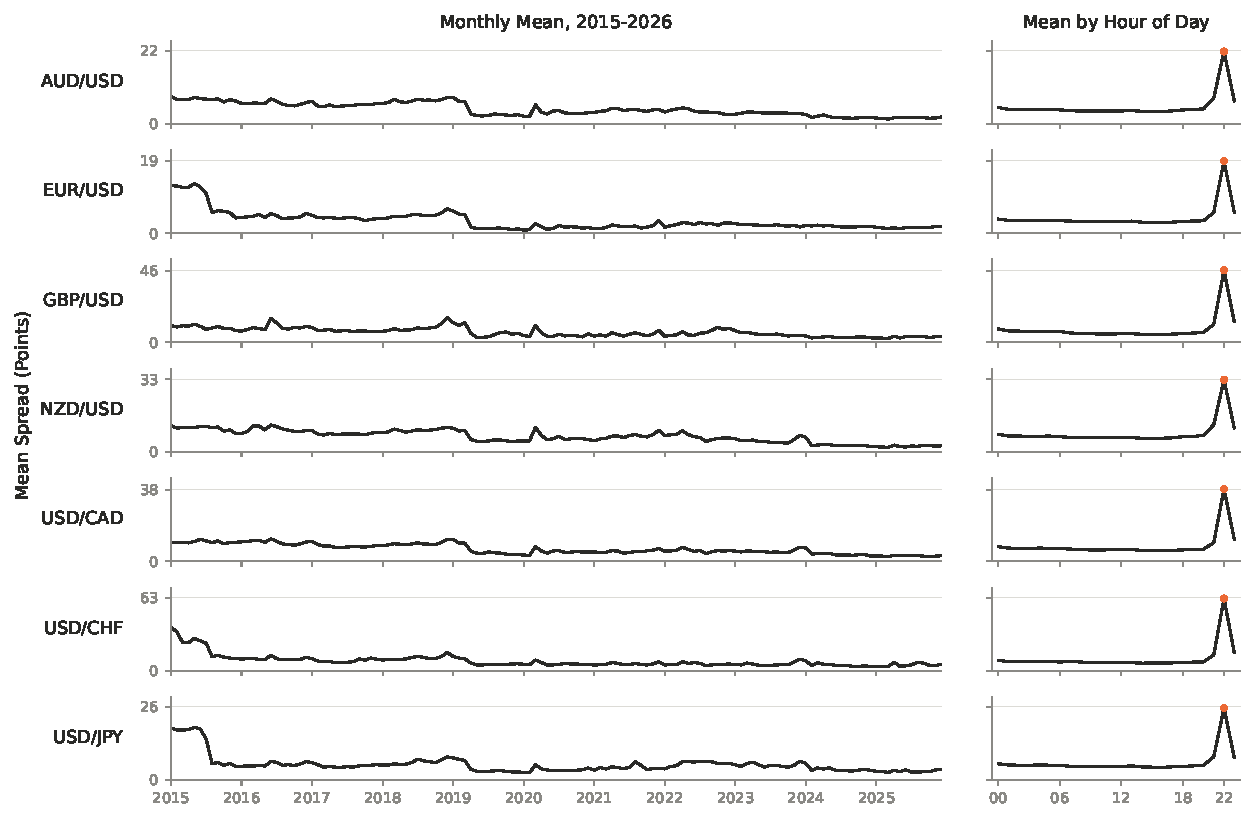
\includegraphics[width=\textwidth]{Images/SpreadOverTime.pdf}
\caption{Monthly mean spread in points for the seven major pairs, 2015 to 2026, computed from the full tick tape. EUR/USD is drawn in black. A model evaluated at a fixed spread is evaluated in market conditions that do not occur in any month of this sample.}
\label{Figure:SpreadOverTime}
\end{figure}

The pattern of this variation matters more than its size. Spreads widen when liquidity falls and around the events that move prices. These are the moments when a model trained on an average spread is most likely to act. A strategy charged a constant spread is therefore charged the wrong amount, and the error is correlated with its own trading activity. The error also goes in the direction that makes the strategy look better.

The engine was validated against cTrader's own backtester, not against itself. Six reference configurations were used, covering two currency pairs and three windows. In all of them, the engine's trade, position, order and deal records reproduce the platform's output byte for byte. The conversion of profit and loss into the account currency was also checked separately against the platform's own figures. The only divergence is sub-pip. It comes from the resolution of the stored quotes, not from the accounting. The engine therefore reproduces the platform it was built against, and it can also do more than that platform. The same strategy is evaluated offline directly on the tick tape. This runs at a speed that the platform's own backtester cannot reach, and over windows that the backtester will not cover. The cost model can be set to any account the broker offers, not only to the account the terminal happens to be connected to.

Two consequences follow. Both are stated here so that \Cref{Chapter:ExperimentalResults} can be read correctly. First, the returns reported in this work are net of the spread actually quoted and of a real commission schedule. They are therefore lower than the same policy would show on bar closes with a fixed spread or no spread, and they cannot be compared directly with results obtained in that way. Second, because the account is swap-free, no financing cost is estimated or left out. A strategy that holds positions over many nights is charged exactly what such an account would charge it.

% !TEX root = ../../Main.tex
\section{Agent Design: Observation, Action and Reward}
\label{Section:AgentDesign}

The environment of \Cref{Section:TradingFramework} supplies prices and charges for trades. Three more decisions are needed to turn it into a reinforcement learning problem: what the agent sees, what it is allowed to do, and what it is rewarded for. This section states these three decisions and then describes the algorithm that learns from them. Each decision is given with the reason for it. In every case the alternative was tried and worked worse, and those failures are part of the result.

\subsection{Observation Space: Indicators, Encoding and Normalisation}

The agent observes a vector of $38$ values at each hourly bar. None of these values is a raw price. A price level carries no information that the agent can generalise from. A policy learned at a price of $1.05$ has no reason to work at $1.20$, and in eleven years of history the price moves by more than that. Every feature is therefore a ratio, and the whole observation is dimensionless. Sixteen technical indicators, listed in \Cref{Tables:Observation}, give the market context. They are split into a fast group, which describes the last hours to days, and a slow group, which describes regimes that last months. This lets the agent tell a move within a trend apart from a change of trend.

% !TEX root = ../Main.tex
\begin{table}[htb!]
\centering
\footnotesize
\caption{The sixteen technical indicators forming the market context of the observation. Periods are in hourly bars. Each moving average contributes two features, its distance from price and its own differential, both in units of the average true range; each momentum reading contributes one, scaled by the movement expected over its lookback.}
\label{Tables:Observation}
\begin{tabularx}{\textwidth}{@{}llrX@{}}
\toprule
\textbf{Indicator} & \textbf{Family} & \textbf{Period} & \textbf{Role in the observation} \\
\midrule
ATR & Volatility & 14 & Volatility unit; divides every trend feature and sets the stop distance \\
\addlinespace
RV (fast) & Volatility & 16 & Short-horizon realised volatility; divides the momentum features \\
RV (slow) & Volatility & 480 & Long-horizon realised volatility; its ratio to the fast reading gives the volatility regime \\
\addlinespace
ER & Trend & 120 & Efficiency ratio; how directional recent movement has been, bounded in $[0, 1]$ \\
\addlinespace
ROC Fast & Momentum & 24 & One day \\
ROC Medium & Momentum & 120 & One week \\
ROC Slow & Momentum & 480 & One month \\
ROC Regime & Momentum & 1{,}440 & One quarter \\
ROC Epoch & Momentum & 2{,}880 & Two quarters \\
\addlinespace
SMA Fast & Trend & 24 & One day \\
SMA Medium & Trend & 120 & One week \\
SMA Slow & Trend & 480 & One month \\
SMA Regime & Trend & 1{,}440 & One quarter \\
SMA Epoch & Trend & 2{,}880 & Two quarters \\
SMA Cycle & Trend & 4{,}320 & Three quarters \\
SMA Era & Trend & 5{,}040 & Roughly one year \\
\bottomrule
\end{tabularx}
\end{table}

The indicator values are encoded as follows. Here $C$ is the bar close, $\sigma_f$ and $\sigma_s$ are the fast and slow realised volatilities, $A$ is the average true range, and $M_i$ is the $i$-th moving average, with period $N_i$:

\begin{equation}
\frac{A}{C}, \qquad \sigma_f, \qquad \ln\!\left(\frac{\sigma_f}{\sigma_s}\right), \qquad \text{ER}
\label{Equation:VolatilityFeatures}
\end{equation}

\begin{equation}
\frac{\text{ROC}(N_j)}{\sigma_f \sqrt{N_j}}, \qquad \frac{C - M_i}{A}, \qquad \frac{M_i - M_i^{-1}}{A}
\label{Equation:TrendFeatures}
\end{equation}

Each formula removes a different dependence. Dividing the average true range by the close gives volatility as a fraction of the price. The logarithm of the ratio of fast to slow volatility shows the volatility regime. It is zero when the two agree, positive when volatility is rising and negative when it is falling. Dividing a momentum reading by $\sigma_f \sqrt{N_j}$ scales it by the movement expected over that lookback under a random walk. A value near one then means a move of normal size, whatever the period. The distance from a moving average, measured in units of the average true range, says how far the price is from its trend compared with the current volatility. The differential of the same quantity gives the direction in which the trend is moving. The other features are the position in the calendar, encoded as four sine and cosine pairs, the current signed exposure as a fraction of the largest position the account could hold, and six values that describe the last bar as log returns of its open, high, low and close against the previous close, divided by $\sigma_f$.

Features that are not bounded by construction are standardised with a causal exponentially weighted z-score, with $\alpha = 1/200$. Here $x_t$ is a raw value, and $\mu_t$ and $s^2_t$ are its running mean and variance:

\begin{equation}
z_t = \frac{x_t - \mu_{t-1}}{\sqrt{s^2_{t-1} + \epsilon}}
\label{Equation:Normalisation}
\end{equation}

\begin{equation}
\mu_t = \mu_{t-1} + \alpha \delta_t, \qquad s^2_t = (1 - \alpha)\left(s^2_{t-1} + \alpha \delta_t^2\right), \qquad \delta_t = x_t - \mu_{t-1}
\label{Equation:NormalisationUpdate}
\end{equation}

The subscript $t-1$ in \Cref{Equation:Normalisation} is the most important detail of this design. A value is standardised with statistics that end at the previous step. Only after that is the value added to those statistics. A z-score computed over the whole sample would leak future information into every observation, and it would inflate every result derived from it. Features that are already bounded, such as the exposure fraction, the efficiency ratio and the calendar encodings, have a flag that skips this layer, so their natural range is kept.

\subsection{Action Space: Position Sizing and Risk}

The agent outputs a single continuous value $a \in [-1, 1]$. Its sign is the direction of the position, and its magnitude is the fraction of a reference size to hold. Direction and size are therefore set by one decision. The discrete action sets reviewed in \Cref{Chapter:RelatedWork} cannot express this. The reference size is fixed-fractional. Let $B$ be the account balance, $\rho$ the risk fraction per position, and $k$ the stop distance in multiples of the average true range. The reference volume $V_{ref}$ is the volume that loses $\rho B$ if the price moves $k \cdot A$ against it. The target volume is this reference scaled by the action:

\begin{equation}
V_{target} = a \cdot V_{ref}, \qquad V_{ref} = \frac{\rho \, B}{k \, A}
\label{Equation:PositionSizing}
\end{equation}

with $\rho = 1\%$ and $k = 1.5$ throughout this work. The agent therefore never chooses an absolute number of units. It chooses a fraction of a size that the risk rule has already set, and this size becomes smaller on its own as volatility rises.

One defect in this calculation was found during the campaign. It is reported here because it affects one of the seven results. The volume calculation leaves out the conversion between the quote currency and the account currency. The risk actually taken is therefore $\rho / p$ and not $\rho$, where $p$ is the price of the pair. For pairs quoted close to one the difference does not matter, and the six pairs quoted against the US Dollar all take about the intended $1\%$. USD/JPY was quoted near $120$ at the start of the sample, so its effective risk is $0.008\%$. This is so small that the computed volume falls below the broker's minimum, and no position can open at all. To correct for this, $\rho$ was scaled by the price. This restores the intended risk per position and does not add leverage. \Cref{Chapter:ExperimentalResults} reports the level used for each pair. The defect is a limitation of the framework, not of the method, and it is listed as future work.

\subsection{Reward Function: Log Return, Scaling and Clipping}

The reward at each step is the log return of account equity, scaled and then clipped:

\begin{equation}
r_t = \operatorname{clip}\!\left(\lambda \ln\!\frac{E_t}{E_{t-1}},\; -c,\; +c\right), \qquad \lambda = 1000, \quad c = 1
\label{Equation:Reward}
\end{equation}

The log return is a natural choice for a trading objective because it is additive over time. The per-step rewards telescope to $\ln(E_T / E_0)$, so maximising their sum maximises the final compounded wealth. The log return also does not depend on the account size. The scale factor is needed, and the reason for it comes from a measured result. Moody and Saffell describe differential risk-adjusted rewards, which accumulate an online estimate of a Sharpe or Sortino ratio. These rewards are scale-invariant: doubling every position leaves the ratio the same. An agent that optimises such a reward gets no gradient that pushes its position size up. In this environment the policy collapses to positions of about $3\%$ of the size available to it. The resulting policy is directionally sensible, but it has no financial value. A scale-sensitive reward is therefore needed. The factor $\lambda$ raises an hourly equity log return, which is usually of order $10^{-4}$, to a magnitude that the critic can distinguish from its own approximation error.

The clip is a numerical safeguard of the kind introduced with the Deep Q-Network \cite{mnih_human-level_2015}. It is applied after the encoding. Its effect must be stated clearly here, because $\lambda$ and $c$ are not independent. Together they clip the raw log return at $\pm c / \lambda = \pm 0.1\%$. On the delivered EUR/USD model the bound is reached on $38.2\%$ of the $68\,155$ hourly steps, and the median absolute scaled reward is $0.70$. So for about two steps in five the agent is told the direction of the equity move but not its magnitude. This is a real property of the objective. It is reported here so that the learned behaviour in \Cref{Chapter:ExperimentalResults} is read against the reward the agent actually received.

\subsection{Learning Algorithm: DDPG and its Adaptations}

The algorithm is the Deep Deterministic Policy Gradient of \Cref{Section:DeepReinforcementLearning}. The actor, the critic and their delayed targets are as described there, and they are trained from a replay buffer with Ornstein-Uhlenbeck exploration noise. The equations of that section are not repeated here. The rest of this section gives the six ways in which the implementation differs from the original, each with its reason. \Cref{Tables:Hyperparameters} compares every value with the published one.

% !TEX root = ../Main.tex
\begin{table}[htb!]
\centering
\footnotesize
\caption{Hyperparameters compared with the original Deep Deterministic Policy Gradient \cite{lillicrap_continuous_2015}. Three values were changed and five mechanisms were added. The rest are the published values.}
\label{Tables:Hyperparameters}
\begin{tabularx}{\textwidth}{@{}llll X@{}}
\toprule
\textbf{Parameter} & \textbf{Original} & \textbf{This work} & \textbf{Status} & \textbf{Reason for the difference} \\
\midrule
Actor hidden layers & $400 \times 300$ & $64 \times 32$ & Changed & Noisy, non-stationary series supports less capacity \\
Discount factor $\gamma$ & $0.99$ & $0.9995$ & Changed & Horizon matched to the holding period, months and not days \\
Hidden normalisation & Batch & Layer & Changed & Inference on one observation must match training on batches \\
\addlinespace
Actor learning rate & $10^{-4}$ & $10^{-4}$ & Unchanged & \\
Critic learning rate & $10^{-3}$ & $10^{-3}$ & Unchanged & \\
Soft update rate $\tau$ & $0.001$ & $0.001$ & Unchanged & \\
Batch size $N$ & $64$ & $64$ & Unchanged & \\
Replay capacity & $10^{6}$ & $10^{6}$ & Unchanged & \\
Critic weight decay & $10^{-2}$ & $10^{-2}$ & Unchanged & \\
Noise $\theta$, $\sigma$ & $0.15$, $0.2$ & $0.15$, $0.2$ & Unchanged & \\
Final layer init & $U[-3\!\times\!10^{-3}, 3\!\times\!10^{-3}]$ & same & Unchanged & \\
\addlinespace
Gradient clip & --- & $1.0$ & Added & Bounds the size of one update caused by a rare large error \\
Warmup transitions & --- & $3{,}000$ & Added & First updates drawn from a varied buffer \\
Actor penalty $\beta$ & --- & $0.001$ & Added & Prevents saturation of the output tangent and collapse to a constant action \\
Reward scale $\lambda$ & --- & $1{,}000$ & Added & Raises an hourly log return above the critic's approximation error \\
Reward clip $c$ & --- & $1$ & Added & Numerical safeguard; limits the raw log return to $\pm 0.1\%$ \\
\bottomrule
\end{tabularx}
\end{table}

The first difference is the observation and the reward, described above.

The second is the size of the networks. The original uses hidden layers of $400$ and $300$ units for low-dimensional control tasks. Here they have $64$ and $32$ units. A $38$-dimensional observation of a noisy, non-stationary series supports much less capacity than a physics simulator with a clean reward. Larger networks fitted the training window but did not generalise beyond it. The third is the discount factor, which was raised from $0.99$ to $0.9995$. With an hourly step, $\gamma = 0.99$ gives a horizon of about a hundred bars, or about four days. This is shorter than the positions this strategy is meant to hold. At $0.9995$ the horizon grows to about two thousand bars, or roughly three months, which matches the regime indicators in the observation.

The fourth is the normalisation inside the networks. The original applies batch normalisation to the hidden layers. This implementation applies layer normalisation instead. The reason is deployment. Batch normalisation behaves differently on a single sample than on a training batch, because it depends on running statistics collected during training. On a live account, the agent must act on exactly one observation at a time. Layer normalisation normalises across the features of one sample. The computation done during training is therefore the same as the computation done in deployment. The target networks also do not need a second set of running statistics that must be kept in sync.

The fifth is gradient clipping. The original uses none. Here the gradient norm of both the actor and the critic is clipped to $1$ before each optimiser step. This limits the size of a single update. It stops a rare large temporal-difference error from moving the parameters far enough to make the critic unstable. It is only a stability measure. In particular, it does not solve the collapse discussed next, which is caused by a lack of gradient, not by too much of it.

The sixth is a penalty on the actor. This is the only change that alters the objective itself, and not just the way it is optimised. It was added because the published algorithm does not train on this problem. The actor's final layer applies a hyperbolic tangent to a pre-activation $u(s)$ to keep the action bounded. The derivative of this function vanishes as $|u|$ grows. If the policy is pushed into that region, it stops responding. The action saturates at $\pm 1$, no gradient flows back, and the agent holds one constant position for the rest of training. The fix is to penalise the magnitude of the pre-activation directly. This keeps the policy in the region where the tangent does not saturate. \Cref{Figure:ActorNetwork} shows where in the network this penalty acts:

\begin{equation}
L_{actor} = -\frac{1}{N}\sum_{i} Q\!\left(s_i, \tanh u(s_i) \,\middle|\, \theta^{Q}\right) + \frac{\beta}{N}\sum_{i} u(s_i)^2
\label{Equation:ActorRegularisation}
\end{equation}

\begin{figure}[htb!]
\centering
\resizebox{\textwidth}{!}{%
\begin{tikzpicture}[
  node distance=5mm,
  layer/.style={draw, rounded corners=1.5pt, align=center, font=\scriptsize, minimum height=9mm, inner sep=3pt, text width=20mm},
  point/.style={draw, circle, inner sep=1.5pt, font=\scriptsize},
  flow/.style={-stealth, semithick},
  pen/.style={-stealth, semithick, dashed}
]
\node[layer] (s) {observation\\$s \in \mathbb{R}^{38}$};
\node[layer, right=of s] (h1) {Linear 64\\LayerNorm\\ReLU};
\node[layer, right=of h1] (h2) {Linear 32\\LayerNorm\\ReLU};
\node[layer, right=of h2] (f3) {Linear 1};
\node[point, right=6mm of f3] (u) {$u$};
\node[layer, right=6mm of u] (th) {$\tanh$};
\node[layer, right=of th] (a) {action\\$a \in [-1,1]$};
\node[font=\scriptsize, below=8mm of u, align=center] (pen) {penalty $\beta\,\overline{u^{2}}$};

\draw[flow] (s) -- (h1);
\draw[flow] (h1) -- (h2);
\draw[flow] (h2) -- (f3);
\draw[flow] (f3) -- (u);
\draw[flow] (u) -- (th);
\draw[flow] (th) -- (a);
\draw[pen] (pen) -- (u);
\end{tikzpicture}}
\caption{The actor. Layer normalisation replaces the batch normalisation of the original, so a single observation is processed exactly as a training batch is. The penalty of \Cref{Equation:ActorRegularisation} acts on the pre-activation $u$, before the tangent. This is where saturation would otherwise remove the gradient.}
\label{Figure:ActorNetwork}
\end{figure}

with $\beta = 0.001$. Setting $\beta = 0$ recovers the original actor loss exactly, so the change extends the original loss and does not replace it. Together with the scale-sensitive reward, this penalty prevents policy collapse. The two mechanisms deal with different parts of the same failure. The reward supplies a gradient that rewards larger positions, and the penalty keeps the actor in the region where that gradient can act. Everything else follows the published algorithm. The learning rates, the soft update rate, the batch size, the replay capacity, the exploration noise parameters, the critic weight decay and the layer initialisation are the values given in the original work. A warmup period of $3000$ transitions is used before learning begins. This way the first updates are drawn from a buffer with some variety in it, and not from the first few correlated steps of an episode.

% !TEX root = ../../Main.tex
\section{Experimental Procedure: Training, Selection and Deployment}
\label{Section:ExperimentalProcedure}

An agent design does not produce a result on its own. Training is stochastic, so the same configuration run twice gives two different policies. A procedure is needed to decide which of them is reported, and why. This section describes that procedure, the criteria used at each stage, and the two deployment decisions that sit between the learned policy and the orders actually sent.

\subsection{Training Procedure: Seeds, Episodes and Data Splits}

The eleven-year window is split once into three consecutive periods. The window is written as $[T_0, T_3)$, where $T_0$ is the first of January 2015 and $T_3$ is the first of January 2026:

\begin{equation}
\underbrace{[T_0, T_1)}_{\text{training, 9 years}} \quad
\underbrace{[T_1, T_2)}_{\text{validation, 1 year}} \quad
\underbrace{[T_2, T_3)}_{\text{testing, 1 year}}
\label{Equation:Split}
\end{equation}

Weights are updated on the training period only. The validation period decides which state of the network is kept. The testing period is used once, after every other decision has been made. Within this split, a single training run works as follows. A seed fixes the network initialisation, the stream of exploration noise and the order in which the replay buffer is sampled, so it determines the whole run. The agent then runs $30$ episodes. An episode is one pass over the training period. Weights are not reset between episodes. The run is a single sequence of $30$ passes, and the network at the start of episode $n+1$ is the network at the end of episode $n$. After each episode the agent is evaluated once over the validation period, with learning turned off. This evaluation is reduced to a single number, the Calmar ratio, which is the annualised return divided by the maximum drawdown. Let $f_n$ be this value and let $g_n$ be an eligibility test defined below. The state kept after episode $n$ is

\begin{equation}
\theta^{\star} \leftarrow \theta_n \quad \text{if} \quad (g_n \wedge \neg g^{\star}) \;\vee\; \left(g_n = g^{\star} \wedge f_n > f^{\star}\right)
\label{Equation:KeepBest}
\end{equation}

which prefers an eligible episode to an ineligible one, whatever the scores. Otherwise it keeps the higher score within the same eligibility class. The saved state is a copy. The run continues training from $\theta_n$, not from $\theta^{\star}$, so a later episode never restarts from an earlier checkpoint. The eligibility test $g_n$ rejects policies that are degenerate. It does not reject a policy only because it performs poorly. An episode passes only if it opened at least ten positions, spent at least three hundred bars on each side of the market, and held its weaker side for at least $30\%$ of the time it held its stronger one. A policy that never trades, or that is long for the whole period, can reach a good Calmar ratio on a trending window without having learned anything about when to hold a position. The test removes such a policy before the scores are compared. Between $128$ and $256$ seeds were run for each currency pair, and the runs differed only in the seed. \Cref{Figure:TrainingPipeline} shows how the three stages fit together.

\begin{figure}[htb!]
\centering
\begin{tikzpicture}[
  node distance=5mm,
  stage/.style={draw, rounded corners=2pt, align=center, font=\small, text width=32mm, minimum height=8mm, inner sep=3pt},
  small/.style={stage, font=\scriptsize, text width=30mm},
  note/.style={font=\scriptsize\itshape, align=left},
  flow/.style={-stealth, thick}
]
\node[stage] (seed) {Seed $s$\\\scriptsize init, noise, sampling};
\node[small, right=10mm of seed] (episode) {Episode $n$ of 30\\one pass over training};
\node[small, right=10mm of episode] (valid) {Validation pass\\learning disabled};
\node[small, below=9mm of valid] (keep) {Calmar $f_n$ + eligibility\\keep-best checkpoint};
\node[small, below=9mm of episode] (test) {Test pass\\once, after 30 episodes};
\node[stage, below=9mm of seed] (pool) {Pool of 128--256\\trained seeds};
\node[stage, below=9mm of pool] (gates) {Gates\\reject degenerate};
\node[small, right=10mm of gates] (sweep) {Risk sweep\\$\times 1.0$ to $\times 3.0$};
\node[small, right=10mm of sweep] (score) {Composite score\\percentile ranks};
\node[stage, below=9mm of gates] (champion) {Published model};

\draw[flow] (seed) -- (episode);
\draw[flow] (episode) -- (valid);
\draw[flow] (valid) -- (keep);
\draw[flow] (keep) -- node[note, above, midway] {} (test);
\draw[flow] (keep.west) to[out=180, in=0] node[note, above, midway] {\scriptsize next episode} (episode.south east);
\draw[flow] (test) -- (pool);
\draw[flow] (pool) -- (gates);
\draw[flow] (gates) -- (sweep);
\draw[flow] (sweep) -- (score);
\draw[flow] (score.south) to[out=270, in=0] (champion.east);
\end{tikzpicture}
\caption{The three stages of the procedure. The Calmar ratio chooses among the episodes of one seed. The composite score of \Cref{Section:ExperimentalProcedure} chooses among seeds.}
\label{Figure:TrainingPipeline}
\end{figure}

One property of this setup must be stated clearly, because it limits what the results in \Cref{Chapter:ExperimentalResults} can claim. The split of \Cref{Equation:Split} applies to the training of a single seed. The choice of which seed to publish, described next, is based on performance over the whole eleven-year window. The performance figures reported in this work are measured over that same window. The testing period is therefore held out from the training of each candidate and from the choice among its episodes. It is not held out from the choice among candidates, so the headline returns are not out-of-sample estimates. This is the weakest point of the method, and it is not hidden anywhere in the rest of this thesis.

\subsection{Model Selection: Gates and Composite Ranking}

Once the seeds for a pair have been trained, each one is evaluated over the full window with the cost model of \Cref{Tables:CostModel}, and one is chosen. The choice is made in two steps, first rejection and then ranking, because they answer two different questions. The first question is whether a policy is admissible at all. The second is which of the admissible policies is best.

Four gates reject a candidate directly. First, its return must be positive. Second, its weaker direction must make up at least $10\%$ of its exposure. This removes policies that are long or short the whole time. Third, its mean holding period must be at least twenty-four bars. This removes policies whose signal is noise. Fourth, its regime score must be higher than the score of the same policy with its position sequence rotated in time. The regime score is the fraction of market movement during which the policy held the correct position. The last gate needs some explanation, because a fixed threshold was tried first and does not work. A rotated policy holds the same positions for the same durations, but at the wrong moments. Its score therefore measures what the policy's autocorrelation and holding pattern would earn by luck alone. Across the seven pairs these null scores range from $48$ to $70$. A fixed threshold of, for example, $55$ would be below chance on one pair and too strict on another. The null score is therefore computed for each model and not assumed.

Candidates that pass the gates are ranked by a composite of percentile ranks within their own pool. For a metric $m$ and a pool of $K$ candidates, the rank of candidate $i$ is

\begin{equation}
R_m(i) = 100 \cdot \frac{\left|\left\{ j : v_m(j) < v_m(i) \right\}\right|}{K - 1}
\label{Equation:PercentileRank}
\end{equation}

where $v_m$ is negated for metrics that are better when smaller, such as drawdown. The metrics are split into three groups, listed in \Cref{Tables:Composite}. The score is the unweighted mean of the three group means:

\begin{equation}
S(i) = \frac{1}{3} \sum_{G \in \{\text{money}, \text{safety}, \text{behaviour}\}} \frac{1}{|G|} \sum_{m \in G} R_m(i)
\label{Equation:Composite}
\end{equation}

% !TEX root = ../Main.tex
\begin{table}[htb!]
\centering
\footnotesize
\caption{Parts of the composite selection score of \Cref{Equation:Composite}. The three groups have equal weight, so return makes up one ninth of the total and does not dominate it. The ratios are those defined in \Cref{Section:PerformanceMeasurement}.}
\label{Tables:Composite}
\begin{tabularx}{\textwidth}{@{}lX@{}}
\toprule
\textbf{Group} & \textbf{Metrics, each used as a percentile rank within the candidate pool} \\
\midrule
Money & Annualised return, Calmar ratio, Sterling ratio \\
\addlinespace
Safety & Sharpe ratio, Sortino ratio, inverse maximum drawdown, inverse downside volatility \\
\addlinespace
Behaviour & Two-sidedness (the weaker exposure side as a fraction of half), regime edge over the model's own rotation null, mean holding period, longest holding period \\
\bottomrule
\end{tabularx}
\end{table}

Two design decisions are built into \Cref{Equation:Composite}. First, ranks are relative to the pool and not absolute. No threshold can therefore exclude a candidate that is simply better than all the others in its pool. Second, the three groups have equal weight, so a policy cannot win on return alone. Money, safety and behaviour each count for a third. A candidate with the highest return in its pool, but with no two-sidedness and no regime edge over its rotation null, scores poorly on two groups out of three. Each candidate that passes the gates is also evaluated at several position sizes, from the reference risk of \Cref{Equation:PositionSizing} up to three times that risk. Scaling the risk fraction changes only the size of the positions the policy takes. It does not change the learned policy. The level chosen for each pair is reported with the results.

\subsection{Deployment: Decision Frequency and Rebalance Threshold}

Two decisions sit between the learned policy and the orders that are actually sent. Together they explain more of the delivered performance than any hyperparameter.

The first is the decision frequency, which is how often the agent may act. The agent observes every hourly bar, but it may act only once per calendar day. A key is built from the timestamp of each bar, and a new action is taken only when that key changes:

\begin{equation}
\kappa(t) = (\text{year}(t), \text{month}(t), \text{day}(t))
\label{Equation:DecisionKey}
\end{equation}

The key is built from the calendar and not from a count of bars. This means that the gaps and short sessions described in \Cref{Section:TradingFramework} do not affect it. A week with a holiday still produces one decision per trading day, and the decisions stay aligned with the trading days. The second decision is a rebalance threshold. A continuous action changes slightly at every decision. Acting on every such change would send a stream of tiny orders, and each of them would pay the spread and a commission. An order is therefore sent only when the change in the target position is large enough to be worth its cost:

\begin{equation}
\left| V_{target} - V_{current} \right| \;\geq\; \max\!\left(V_{min},\; \eta \left| V_{ref} \right|\right), \qquad \eta = 0.20
\label{Equation:Hysteresis}
\end{equation}

where $V_{min}$ is the broker's minimum volume. The threshold is a fraction of the reference volume, not of the position currently held, so it does not shrink to zero as a position is reduced. \Cref{Tables:Deployment} isolates the effect of each decision, measured on one model with nothing retrained. The comparison is between four configurations of the same weights, so the differences are attributable to the deployment layer alone.

% !TEX root = ../Main.tex
\begin{table}[htb!]
\centering
\footnotesize
\caption{Effect of the two deployment decisions, measured on one EUR/USD model over the full window with nothing retrained. All four rows use the same weights with different execution settings, so the differences are attributable to the deployment layer alone. This model comes from before the seven-pair campaign and is used here only to isolate the effect of each decision.}
\label{Tables:Deployment}
\begin{tabular}{@{}llrrrr@{}}
\toprule
\textbf{Frequency} & \textbf{Threshold} & \textbf{Commission} & \textbf{Return} & \textbf{Sharpe} & \textbf{Max drawdown} \\
\midrule
Daily & --- & none & $+42.48\%$ & $0.319$ & $24.4\%$ \\
Hourly & --- & none & $-38.57\%$ & $-0.308$ & $50.5\%$ \\
Hourly & --- & 3.5 points & $-64.70\%$ & $-0.732$ & $70.5\%$ \\
Daily & $0.20$ & 3.5 points & $+34.02\%$ & $0.275$ & $23.5\%$ \\
\bottomrule
\end{tabular}
\end{table}

Two things follow from that table. First, moving from hourly to daily decisions adds about eighty percentage points and turns a losing configuration into a profitable one. The reason is that hourly decisions act on noise that the eleven-year horizon of the discount factor was never meant to capture. Second, the rebalance threshold recovers about twelve percentage points under realistic costs, and at the same time it reduces drawdown instead of increasing it. This is unusual. Commission alone costs over twenty percentage points without the filter and about six with it. The continuous action space makes the strategy expressive, and this filter keeps its trading costs low enough.

\subsection{Worked Example: One Position From Decision to Settlement}

The earlier parts of this chapter define each component separately. This section follows one position through all of them, using a trade taken by the delivered EUR/USD model. This allows the arithmetic to be checked instead of taken on trust.

At 02:00 on 30 January 2019 the daily decision key of \Cref{Equation:DecisionKey} changed, and the agent was asked for an action for the first time that day. It received the 38-value observation of \Cref{Section:AgentDesign}, built from the bar that had just closed, and it returned a positive action. At that moment the reference volume of \Cref{Equation:PositionSizing} risked $1\%$ of the balance over a stop of $1.5$ average true ranges. The action scaled this volume, and the result was rounded to the broker's volume step. This gave a target of $12{,}000$ units of the base currency. The change from the position held at that time was larger than the threshold of \Cref{Equation:Hysteresis}, so an order was sent. The tick recorded at that instant quoted $1.14392$ ask and $1.14387$ bid, a spread of five points. The buy was filled at the ask. Twenty-four hours later the key changed again, and the agent's action changed sign. The position was closed at the bid quoted at that time, $1.14931$. The profit follows from those two prices and the volume. It is expressed in the account currency at the conversion rate recorded on the closing tick:

\begin{equation}
12{,}000 \times \left(1.14931 - 1.14392\right) = 64.68 \text{ USD} \;\;\longrightarrow\;\; 56.27 \text{ EUR}
\label{Equation:WorkedGross}
\end{equation}

The spread is already included in that figure. It was paid at entry, by filling at the ask and not at the mid, and again at exit, by filling at the bid. This is why the round trip crosses the spread exactly once. The commission is charged separately at both ends:

\begin{equation}
2 \times 3.5 \times 10^{-5} \times 12{,}000 = 0.84 \text{ USD} \;\;\longrightarrow\;\; 0.72 \text{ EUR}
\label{Equation:WorkedCommission}
\end{equation}

The position was held overnight, but the swap is zero because the account is swap-free. The position therefore settled at $56.27 - 0.72 = 55.55$ EUR, which is the figure in the exported trade record. One trade says little on its own. The delivered EUR/USD model took $1{,}777$ trades over the eleven years. Across all of them, the same accounting gives a gross profit of $8{,}733.62$ EUR, a commission charge of $1{,}669.50$ EUR and a swap charge of exactly zero, for a net of $7{,}064.12$ EUR. Commission alone took $19.1\%$ of the gross profit. This figure does not include the spread, which cannot be separated from the gross figure because it is part of every fill. A result reported without these charges would describe a different strategy.

Everything described here was fixed before any result was seen. There is one architecture, one observation, one reward and one selection rule, and they were applied unchanged to seven instruments. This is what makes the results comparable across pairs.

It also makes the results falsifiable, because they can show the design to be wrong. A design that is tuned on one instrument until it works can always be made to work on that instrument. Its results then cannot tell a real strategy apart from a description of that instrument's past prices. When the same design is applied to seven instruments, a failure on any of them shows in the results. The results in \Cref{Chapter:ExperimentalResults} include a pair on which the design does not work.
%
% !TEX root = ../../Main.tex
\fancychapter{Experimental Results}
\label{Chapter:ExperimentalResults}

This chapter reports the results of the design of \Cref{Chapter:Implementation}. Seven agents were trained, one for each major currency pair. Each agent was evaluated over eleven years under the cost model of \Cref{Tables:CostModel}. Every figure below comes from a stored run that can be opened again. The analysis was computed again from those runs. It was not copied from the training logs.

The order of this chapter was chosen on purpose. The returns come first. Then come the checks that decide whether those returns mean anything, then the year that was held back, and last the result of running the seven agents together.

% !TEX root = ../../Main.tex
\section{Evaluation Protocol}
\label{Section:EvaluationProtocol}

The account, the cost model and the execution engine are described in \Cref{Section:TradingFramework} and are not repeated here. Three points are specific to the evaluation.

The evaluation window runs from 1 January 2015 to 1 January 2026, which is eleven years. It starts one year after the data begins. This way the slowest indicator in the observation, a moving average over five thousand hourly bars, is fully warmed up before the first decision.

Every result is measured from five different starting balances: $9\,900$, $10\,000$, $10\,050$, $10\,100$ and $10\,200$ euros. A strategy whose result depends on its starting point is not a real strategy. Small changes to the opening balance change the rounding of every position size, and so they change the whole sequence of trades. Reporting one balance would hide this sensitivity. The tables therefore give the mean across the five balances and the dispersion around it.

Position size is a parameter set for each pair separately. It was chosen by the sweep described in \Cref{Section:ExperimentalProcedure} and was not fixed in advance. Five pairs use the reference risk of \Cref{Equation:PositionSizing}. NZD/USD uses one and a half times that risk, and USD/JPY uses a smaller fraction of it. Position size scales every trade, but it does not change the policy that chooses the trades. The ratios, the alpha and beta decomposition and the correlation structure are therefore not affected by it.

% !TEX root = ../../Main.tex
\section{Benchmarks and Performance Metrics}

The benchmark is to buy the pair at the start of the window and hold it to the end. This is the fair comparison for a directional strategy on a single instrument. Anyone can do it, and it costs one spread. A strategy that cannot beat it does not justify its extra complexity. The thesis proposal named a random-signal baseline and a moving-average crossover instead. Both were dropped, because a trader would not hold either of them as a real alternative.

The reported metrics are those defined in \Cref{Section:PerformanceMeasurement}: total and annualised return, the Sharpe, Sortino, Calmar and Sterling ratios, maximum drawdown and the number of trades. \Cref{Tables:PerformanceMetrics} states what each one measures. All ratios use a risk-free rate of zero. They can therefore be compared across pairs without any assumption about interest rates.

% !TEX root = ../Main.tex
\begin{table}[htb!]
\centering
\footnotesize
\caption{Summary of the performance metrics used in this work.}
\label{Tables:PerformanceMetrics}
\begin{tabularx}{\textwidth}{@{}lX@{}}
\toprule
\textbf{Metric} & \textbf{Description} \\
\midrule
Net Profit & Total profit or loss \\
\addlinespace
Profit Factor & Ratio of gross profit to gross loss \\
\addlinespace
Commission and Swap & Costs that reduce net profit \\
\addlinespace
Max Balance and Equity Drawdown & Largest losses observed \\
\addlinespace
Total Trades and Winning Trades & How much the strategy trades and how often it wins \\
\addlinespace
Max Consecutive Winning and Losing Trades & How consistent the results are \\
\addlinespace
Largest Winning and Losing Trades & How large single gains or losses can be \\
\addlinespace
Average Trade & Average result per trade, a measure of trading efficiency \\
\addlinespace
Sharpe Ratio and Sortino Ratio & Risk-adjusted return \\
\bottomrule
\end{tabularx}
\end{table}

For four of them, it is worth saying why all four are reported instead of choosing one. Return says how much was made. It says nothing about the risk taken to make it. The Sharpe ratio divides return by total volatility. This penalises a strategy for moving up as much as for moving down. The Sortino ratio corrects this by counting only downside movement. Calmar and Sterling divide by drawdown instead of volatility. Calmar uses the worst loss ever suffered and Sterling the average one. They therefore measure how far the account fell, and not how volatile it was, which is the question an investor asks. A strategy can look strong on one of these and weak on another. Where that happens in this work, the text points it out.

One point applies to every number in this chapter. Returns are net of the spread quoted at the moment of each trade and of the account commission in \Cref{Tables:CostModel}. They therefore cannot be compared with results computed on bar closes with a fixed spread or with no spread. They are also lower than the same policies would show under those conditions.

% !TEX root = ../../Main.tex
\section{Results Across the Seven Majors}
\label{Section:PairResults}

\Cref{Tables:PairResults} gives the result for each pair, in alphabetical order. Total return over the eleven years goes from $+226.6\%$ on USD/CAD, the highest, to $+15.7\%$ on USD/JPY, the lowest. Every pair is profitable, and every pair is profitable from all five starting balances.

% !TEX root = ../Main.tex
\begin{table}[htb!]
\centering
\footnotesize
\caption{Result for each pair from 2015 to 2026. The return columns give the mean, standard deviation and range across the five starting balances of \Cref{Section:EvaluationProtocol}. Every pair is profitable from all five. Ratios and drawdown are from the reference run. USD/CAD returns the most, and USD/CHF is best on every risk measure.}
\label{Tables:PairResults}
\begin{tabular}{@{}lrrrrrrrrr@{}}
\toprule
\textbf{Pair} & \textbf{Mean} & \textbf{SD} & \textbf{Min} & \textbf{Max} & \textbf{Sharpe} & \textbf{Sortino} & \textbf{Calmar} & \textbf{Max DD} & \textbf{Trades} \\
\midrule
AUD/USD & 102.5\% & 10.6 & 87.2\% & 117.1\% & 0.348 & 0.496 & 0.143 & 41.1\% & 1,561 \\
EUR/USD & 73.9\% & 3.3 & 69.5\% & 77.8\% & 0.387 & 0.544 & 0.106 & 46.8\% & 1,778 \\
GBP/USD & 124.1\% & 5.1 & 115.1\% & 129.1\% & 0.397 & 0.563 & 0.155 & 50.4\% & 2,516 \\
NZD/USD & 56.4\% & 3.8 & 52.2\% & 61.7\% & 0.368 & 0.531 & 0.187 & 23.3\% & 1,011 \\
USD/CAD & \textbf{226.6\%} & 10.8 & 216.9\% & 246.0\% & 0.603 & 0.870 & 0.228 & 49.1\% & 2,213 \\
USD/CHF & 50.6\% & 5.2 & 43.4\% & 56.4\% & \textbf{0.802} & \textbf{1.552} & \textbf{0.492} & \textbf{8.2\%} & 220 \\
USD/JPY & 15.7\% & 0.7 & 14.5\% & 16.5\% & 0.251 & 0.342 & 0.057 & 24.0\% & 1,438 \\
\bottomrule
\end{tabular}
\end{table}

One fact is important for everything that follows, and it is easy to miss. \textbf{Five of the seven pairs lost value over the eleven years.} A trader who had simply bought and held would have finished down $26.1\%$ on NZD/USD, $20.3\%$ on USD/CHF, $18.2\%$ on AUD/USD, $13.5\%$ on GBP/USD and $2.9\%$ on EUR/USD. Only USD/CAD, at $+18.1\%$, and USD/JPY, at $+30.7\%$, rose. The agents made money on all seven. On five of them, the return was therefore earned in a falling market, and not in a rising one.

% !TEX root = ../Main.tex
\begin{table}[htb!]
\centering
\footnotesize
\caption{Each agent against buying and holding its own pair over the same window and under the same costs. Five of the seven pairs lost value over the eleven years, so on those the return was earned against a falling market. USD/JPY is the only pair whose benchmark rose substantially, and the only one the agent failed to beat.}
\label{Tables:Benchmark}
\begin{tabular}{@{}lrrrr@{}}
\toprule
\textbf{Pair} & \textbf{Market} & \textbf{Model} & \textbf{Excess} & \textbf{Positive Years} \\
\midrule
AUD/USD & $-18.2\%$ & $+87.2\%$ & $+105.4$ pp & 8 of 11 \\
EUR/USD & $-2.9\%$ & $+70.6\%$ & $+73.4$ pp & 5 of 11 \\
GBP/USD & $-13.5\%$ & $+129.1\%$ & $+142.5$ pp & 7 of 11 \\
NZD/USD & $-26.1\%$ & $+60.1\%$ & $+86.1$ pp & 7 of 11 \\
USD/CAD & $+18.1\%$ & $+221.0\%$ & $+202.9$ pp & 8 of 11 \\
USD/CHF & $-20.3\%$ & $+54.8\%$ & $+75.2$ pp & \textbf{10 of 11} \\
USD/JPY & $+30.7\%$ & $+16.2\%$ & $\mathbf{-14.4}$ pp & 5 of 11 \\
\bottomrule
\end{tabular}
\end{table}

The rest of this section discusses each pair in turn, in alphabetical order. For each pair it covers what the market did, what the agent returned in comparison, how that return decomposes into policy and market exposure, what the agent paid in costs, and how it traded.

\subsection{AUD/USD}

The Australian Dollar fell $18.2\%$ against the US Dollar over the eleven years. The agent returned $+87.2\%$, which is $105.4$ percentage points above holding the pair. It earned this from the short side: only $27.9\%$ of its $1\,561$ positions were long.

This result needs care in the alpha and beta decomposition. Its beta of $-2.013$ is the largest negative beta of the seven. This means that the agent was short the falling market at roughly twice its size. Of its $8.18\%$ mean yearly return, $4.96$ points are alpha and $3.22$ points are beta return, from the general fall of the market. Close to two fifths of what it earned therefore came from the Australian Dollar falling, and not from choosing when to be short. The policy does make a profit, but part of that profit would turn into a loss in a decade where the pair rose.

It trades at a moderate pace. Its median holding period is $9.7$ days, its average size is $0.77$ of the reference size, and its win rate is $52.7\%$. It made $10\,689$ euros of gross profit and paid $2\,200$ in commission. That is a $20.6\%$ share, the highest of the seven, and it comes directly from its turnover. The equity curve is uneven. Eight of eleven years are positive. The best year is 2024, at $+72.4\%$ and $81.6$ points above the benchmark, and the worst is 2017, at $-22.5\%$. Its maximum drawdown is $41.1\%$.

\begin{figure}[htb!]
\centering
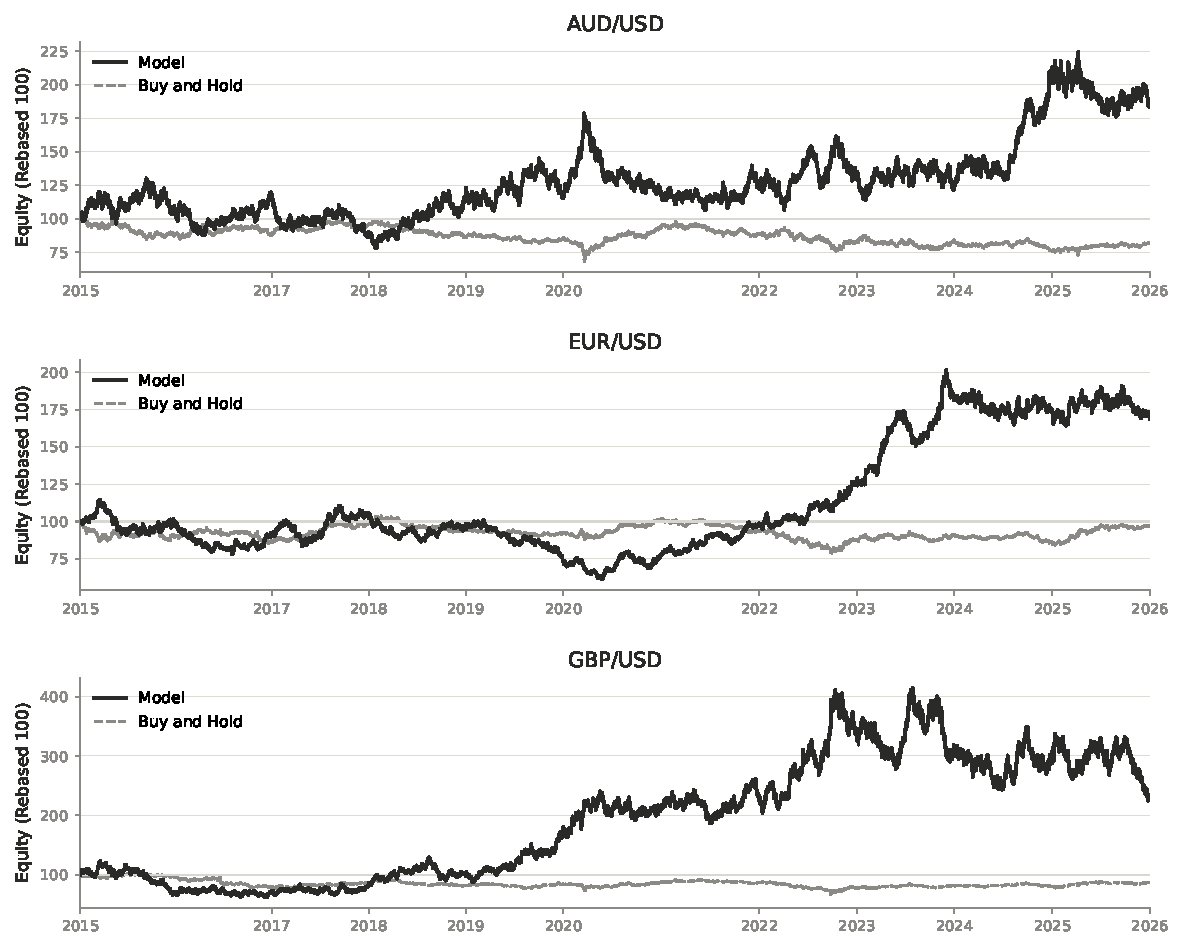
\includegraphics[width=\textwidth]{Images/PairEquityA.pdf}
\caption{AUD/USD, EUR/USD and GBP/USD against buying and holding the same pair, rebased to 100. All three benchmarks finish below their starting level.}
\label{Figure:PairEquityA}
\end{figure}

\subsection{EUR/USD}

EUR/USD is the clearest example in this work of a return that does not come from market exposure. The pair finished almost exactly where it started, down $2.9\%$ over eleven years, and the agent returned $+70.6\%$. Its beta is $+0.266$, and market exposure adds $0.01$ percentage points per year. Of a $6.63\%$ mean yearly return, $6.62$ points are therefore attributable to the policy. The market had no trend for the agent to follow, so the return came from timing alone.

It has the shortest holding period of the seven, a median of $3.9$ days, and it trades at a low $0.40$ of the reference size. Its exposure is close to balanced, with $55.5\%$ long across $1\,778$ positions. It won $51.9\%$ of them. Gross profit of $8\,734$ euros became $7\,064$ after $1\,669$ euros of commission, a $19.1\%$ share.

The equity curve in \Cref{Figure:PairEquityA} shows that the headline return also needs care here, for a different reason than on AUD/USD. Only five of eleven years are positive. The agent is roughly flat for the first six years of the window. It makes almost all of its return between 2021 and 2023, when the pair moved in unusually wide ranges: $+27.3\%$, $+29.0\%$ and $+44.0\%$ in those three years, against $-25.3\%$ in 2019. This policy needs volatility to work. Its maximum drawdown of $46.8\%$ comes from the periods when there was not enough volatility.

\subsection{GBP/USD}

GBP/USD has the highest alpha of the seven, at $+11.64\%$ per year, with a beta of $-0.054$ that is statistically indistinguishable from zero. Its mean yearly return is $11.70\%$, and only $0.06$ points of it come from market exposure. It is as close to pure policy as any result in this chapter. Sterling itself fell $13.5\%$ over the window, so the agent's $+129.1\%$ is $142.5$ percentage points above the benchmark.

It is the most active model, with $2\,516$ positions. It also holds them the longest of the six working agents, with a median of $12.6$ days. It therefore keeps many positions open at the same time, and does not trade quickly. It trades near full size, at $0.89$, and wins $51.3\%$ of the time. Gross profit was $16\,630$ euros against $3\,168$ of commission, which left $13\,462$.

Its returns come mostly from the years when sterling moved sharply. These show in \Cref{Figure:PairEquityA} as two steep sections: $+82.2\%$ in 2019 and $+52.0\%$ in 2022. \Cref{Section:TradingBehaviour} looks at the second of these in detail. The same aggressive trading also produces the worst single year of any agent, $-31.6\%$ in 2015, and the deepest drawdown, $50.4\%$. Seven of eleven years are positive. This is the most volatile of the profitable models. A reader should weigh its alpha against a drawdown that halved the account.

\subsection{NZD/USD}

The New Zealand Dollar fell the most of the seven, $26.1\%$ over the window. The agent returned $+60.1\%$, an excess return of $86.1$ points over the benchmark. Like AUD/USD, it traded mostly from the short side, with $24.0\%$ of positions long and a beta of $-0.708$.

Its alpha of $+2.79\%$ per year is the smallest of the six profitable models. Of its $4.62\%$ mean return, $1.83$ points are beta return. A large part of what it earned, though less than half, therefore came from the market falling and not from timing. By alpha and beta, it is the weakest of the six that worked.

\Cref{Figure:PairEquityB} shows it next to USD/CAD and USD/CHF. This agent is careful, and its risk numbers show the benefit. It takes the fewest positions of the active models, $1\,011$, and holds an average of $0.24$ of the reference size. Its maximum drawdown is $23.3\%$, the second lowest of the seven. Its Calmar ratio of $0.187$ is better than that of four pairs that returned much more. This shows why return is measured against drawdown, and not on its own. Gross profit was $7\,314$ euros and commission $1\,424$, a $19.5\%$ share. Seven of eleven years are positive. The best is 2022 at $+14.5\%$ and the worst is 2016 at $-6.4\%$. It is the steadiest of the models of moderate size.

\begin{figure}[htb!]
\centering
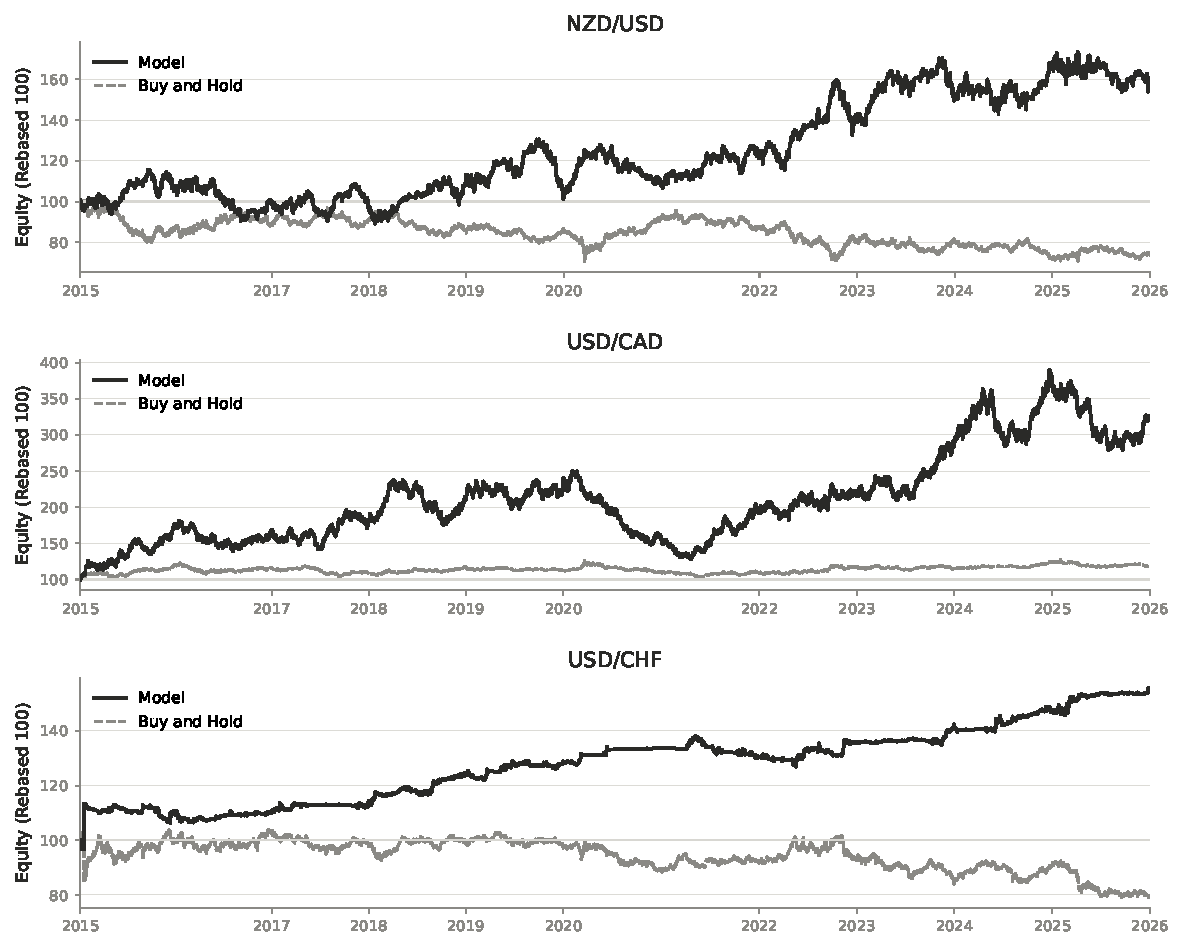
\includegraphics[width=\textwidth]{Images/PairEquityB.pdf}
\caption{NZD/USD, USD/CAD and USD/CHF against buying and holding the same pair, rebased to 100. USD/CAD is the only one of the three whose benchmark rises.}
\label{Figure:PairEquityB}
\end{figure}

\subsection{USD/CAD}

USD/CAD returned $+226.6\%$, by far the largest total in this work. It is also the result that must be read most carefully. Its beta of $+2.393$ is the highest of the seven, and the pair itself rose $18.1\%$. The agent was therefore long a rising market at more than twice its size. Of a $14.23\%$ mean yearly return, $4.21$ points are beta return and $10.02$ are alpha.

That alpha is real, and it is the second highest of the seven. So the model does not look good only because its market went up. But leverage is symmetric: it raises losses as much as gains, and the yearly record shows both. The best year is 2015, at $+71.7\%$ and $52.7$ points above the benchmark. The worst is 2020, at $-34.8\%$. Its maximum drawdown is $49.1\%$, and recovering from a $49\%$ drawdown needs a $96\%$ gain. Eight of eleven years are positive.

It is the second most active model, with $2\,213$ positions and a median holding period of $5.7$ days. It trades at $0.79$ of the reference size and has the highest win rate of the seven, at $55.0\%$. It also earned the most in euros, $25\,577$ gross, and paid $3\,432$ in commission. That is a $13.4\%$ share, lower than for the four pairs discussed above, because its profit per position was larger.

\subsection{USD/CHF}

USD/CHF returned $+54.8\%$. It is fifth of seven on return and first on every risk-adjusted measure. Its Sharpe ratio of $0.802$, Sortino ratio of $1.552$ and Calmar ratio of $0.492$ are the highest of the seven. Its maximum drawdown of $8.2\%$ is a sixth of the worst. The Swiss Franc strengthened over the period, so the pair fell $20.3\%$. With a beta of $-0.082$, the agent took almost none of that movement: of a $4.07\%$ mean yearly return, $3.91$ points are alpha.

Its trading explains all of these numbers. It takes $220$ positions in eleven years, roughly one every eighteen days. It holds an average of $0.09$ of its reference size, a tenth of what it is allowed. Because it trades so little, it pays almost nothing to trade: $130$ euros of commission against $5\,587$ of gross profit. That is a $2.3\%$ share, where the average of the seven is $16.0\%$. It keeps $97.7\%$ of what it earns, while AUD/USD keeps $79.4\%$.

It is positive in ten of eleven years, the most consistent record in this work, and its worst year is $-2.4\%$. Its win rate of $49.8\%$ is the lowest of the seven. This point deserves attention. The best model of the seven is wrong slightly more often than a coin toss. It is still the best because of how it sizes and holds the positions it gets right. It is also the only model that made money in the held-out year of \Cref{Section:OutOfSample}. On return alone it would have placed fifth and would not have been chosen. The selection criteria of \Cref{Section:ExperimentalProcedure} are there to prevent this.

\subsection{USD/JPY}

USD/JPY is the one failure of the seven, and it is the only pair whose benchmark rose by a large amount. The pair gained $30.7\%$ over the window, while the agent returned $+15.7\%$. It finished $14.4$ percentage points behind an investor who bought the pair and did nothing. Its beta of $+1.012$ and its correlation of $+0.946$ with the pair's own yearly move show what it became: a plain long position in the pair, with extra trading and extra costs. Its alpha is $-1.08\%$ per year, the only negative figure in \Cref{Tables:AlphaBeta}.

Every position it takes is long. Its median holding period is measured in years, not days. Its average action is $0.98$. This means it holds almost full size all the time and no longer makes a sizing decision at all. It earned $1\,761$ euros gross, the least of the seven, and paid $155$ in commission. Five of eleven years are positive.

\begin{figure}[htb!]
\centering
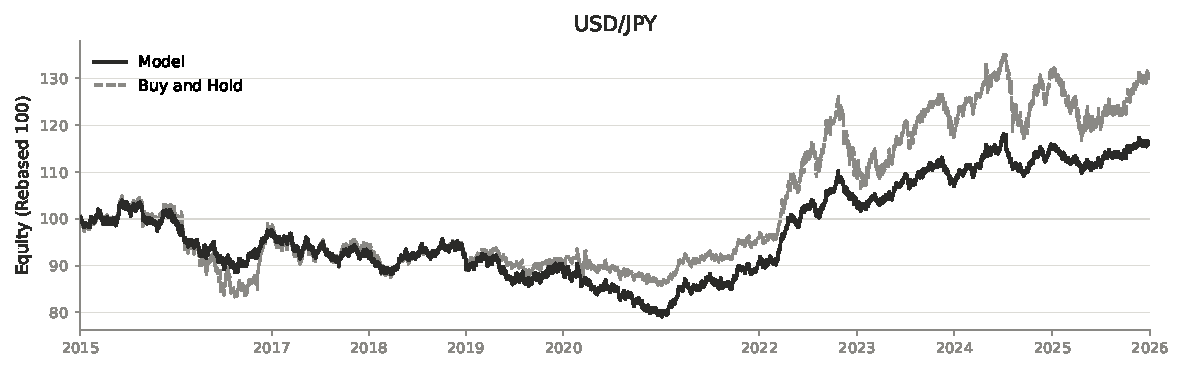
\includegraphics[width=\textwidth]{Images/PairEquityC.pdf}
\caption{USD/JPY against buying and holding the pair. The two lines move closely together. This is what a beta of $+1.012$ looks like, and it is the reason this result is reported as a failure.}
\label{Figure:PairEquityC}
\end{figure}

\Cref{Figure:PairEquityC} shows this more clearly than the statistics do: the model and the benchmark move together, with the model slightly below. \Cref{Section:NegativeResult} explains the cause and what was tried to fix it.

% !TEX root = ../../Main.tex
\section{Trading Behaviour: How the Agents Actually Trade}
\label{Section:TradingBehaviour}

A return figure says whether an agent made money. It says nothing about how, and here that matters for a specific reason. The main claim of this work is that a continuous action lets one decision set both the direction and the size of a position. If the agents had learned to use only the two ends of that action, they would be discrete traders with extra machinery, and the claim would mean nothing. This section examines what they did in practice.

\subsection{Use of the Continuous Action}

The agent outputs an action $a \in [-1, 1]$ and holds $|a|$ of the reference size defined in \Cref{Equation:PositionSizing}. \Cref{Figure:ActionDistribution} shows how this value is distributed over the whole evaluation window for each pair.

% !TEX root = ../Main.tex
\begin{table}[htb!]
\centering
\footnotesize
\caption{Trading behaviour over the evaluation window. Mean $|a|$ is the average absolute action, that is, the average fraction of the reference position size held while in the market. Win rate is the share of closed positions with a positive net result after costs.}
\label{Tables:Behaviour}
\begin{tabular}{@{}lrrrrrr@{}}
\toprule
\textbf{Pair} & \textbf{Positions} & \textbf{Long} & \textbf{Median Hold} & \textbf{Longest Hold} & \textbf{Win Rate} & \textbf{Mean $|a|$} \\
\midrule
AUD/USD & 1,561 & 27.9\% & 9.7 d & 227 d & 52.7\% & 0.77 \\
EUR/USD & 1,778 & 55.5\% & 3.9 d & 43 d & 51.9\% & 0.40 \\
GBP/USD & 2,516 & 46.9\% & 12.6 d & 149 d & 51.3\% & 0.89 \\
NZD/USD & 1,011 & 24.0\% & 5.9 d & 119 d & 52.8\% & 0.24 \\
USD/CAD & 2,213 & 65.6\% & 5.7 d & 97 d & 55.0\% & 0.79 \\
USD/CHF & 220 & 34.2\% & 8.0 d & 345 d & 49.8\% & 0.09 \\
USD/JPY & 1,438 & 100.0\% & 2,120 d & 4,004 d & 50.7\% & 0.98 \\
\bottomrule
\end{tabular}
\end{table}

\begin{figure}[htb!]
\centering
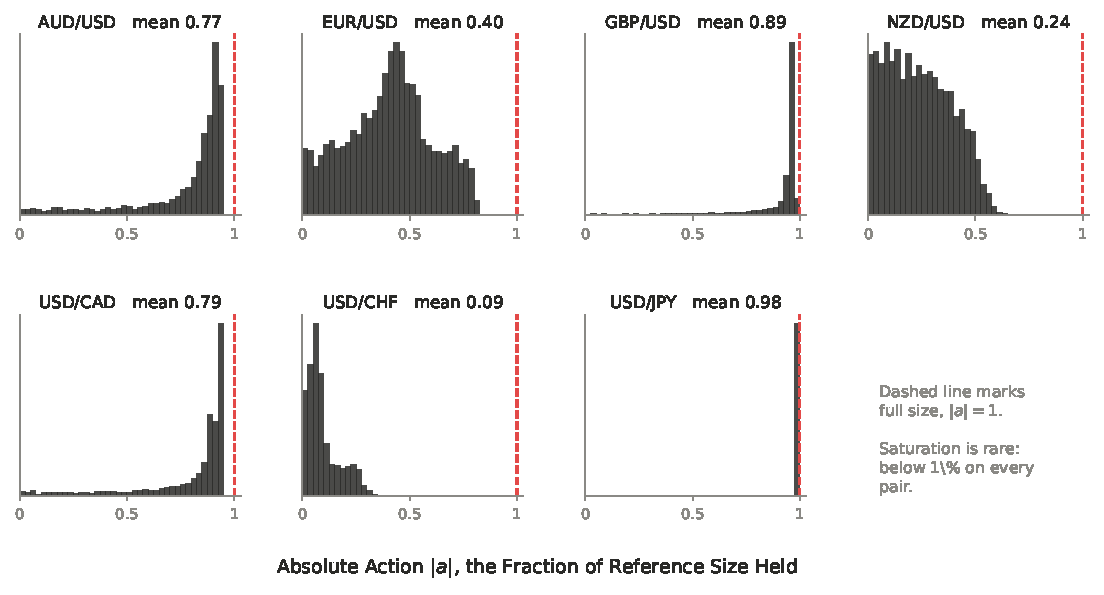
\includegraphics[width=\textwidth]{Images/ActionDistribution.pdf}
\caption{Distribution of the absolute action over the evaluation window. The dashed line marks full size. If the agents had turned the continuous action into a discrete one, these histograms would be concentrated against that line. Instead, most of the mass lies inside the range.}
\label{Figure:ActionDistribution}
\end{figure}

The action does not saturate at $+1$ or $-1$. On every pair, fewer than one percent of decisions are above $|a| = 0.98$, and on six of the seven pairs the figure is zero to one decimal place. The mean absolute action goes from $0.09$ on USD/CHF to $0.98$ on USD/JPY. The agents therefore settled on very different position sizes from the same design and the same reference risk.

This dispersion of sizes is informative in itself. USD/CHF holds roughly a tenth of the size available to it. This is why its maximum drawdown is $8.2\%$ while its Sharpe ratio is the highest of the seven. It found a small advantage and kept its size small to match, instead of pushing it harder. NZD/USD, at $0.24$, behaves in a similar way. USD/JPY is at the other end, with $0.98$. This number is the symptom of the failure described in \Cref{Section:NegativeResult}: an agent that always holds full size in one direction no longer makes a sizing decision at all.

The sizing also adapts in a second way, which the histogram does not show. The reference size is inversely proportional to the average true range, so the same action gives a smaller position when volatility rises. The action and the volatility scaling combine, and the position held is the product of the two.

\subsection{Direction, Size and Outcome Together}

\Cref{Figure:DecisionAnatomy} follows EUR/USD over three years. It shows the price, the action of the agent, the position it held as a result, and the equity that followed.

\begin{figure}[htb!]
\centering
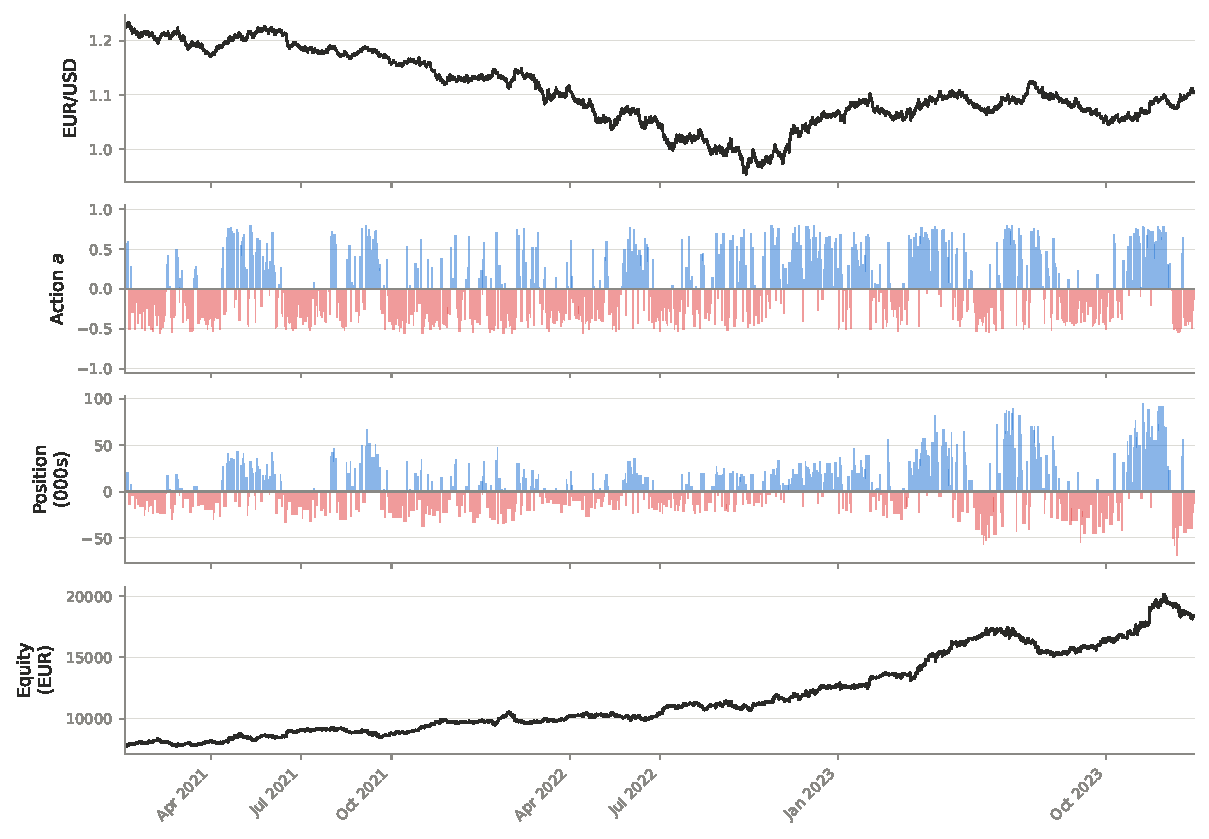
\includegraphics[width=\textwidth]{Images/DecisionAnatomy.pdf}
\caption{EUR/USD from 2021 to 2024. From top: the price; the action, positive for long and negative for short; the resulting net position in thousands of units; and account equity. The action changes sign well before the position does, because a change is only acted on when it is larger than the threshold of \Cref{Equation:Hysteresis}.}
\label{Figure:DecisionAnatomy}
\end{figure}

Three behaviours can be seen. First, the action moves continuously and does not switch between fixed levels. Its magnitude changes as much as its sign. Second, the position follows the action, but in larger steps, because the rebalance threshold blocks small adjustments. Long periods of constant position are periods where the agent kept changing its target by less than the threshold. Third, the sign does not change often. Over the three years the agent reverses direction a few dozen times. This fits the daily decision frequency, and does not fit an agent that reacts to every bar it observes.

\subsection{Trend Identification and Reversal}

The clearest example of an agent holding a position through a sustained move is GBP/USD in the second half of 2022, shown in \Cref{Figure:TrendRide}. Sterling fell from $1.22$ to below $1.04$ over roughly ten weeks, a fall of more than fifteen percent. The steepest part came after the United Kingdom fiscal announcement of late September.

\begin{figure}[htb!]
\centering
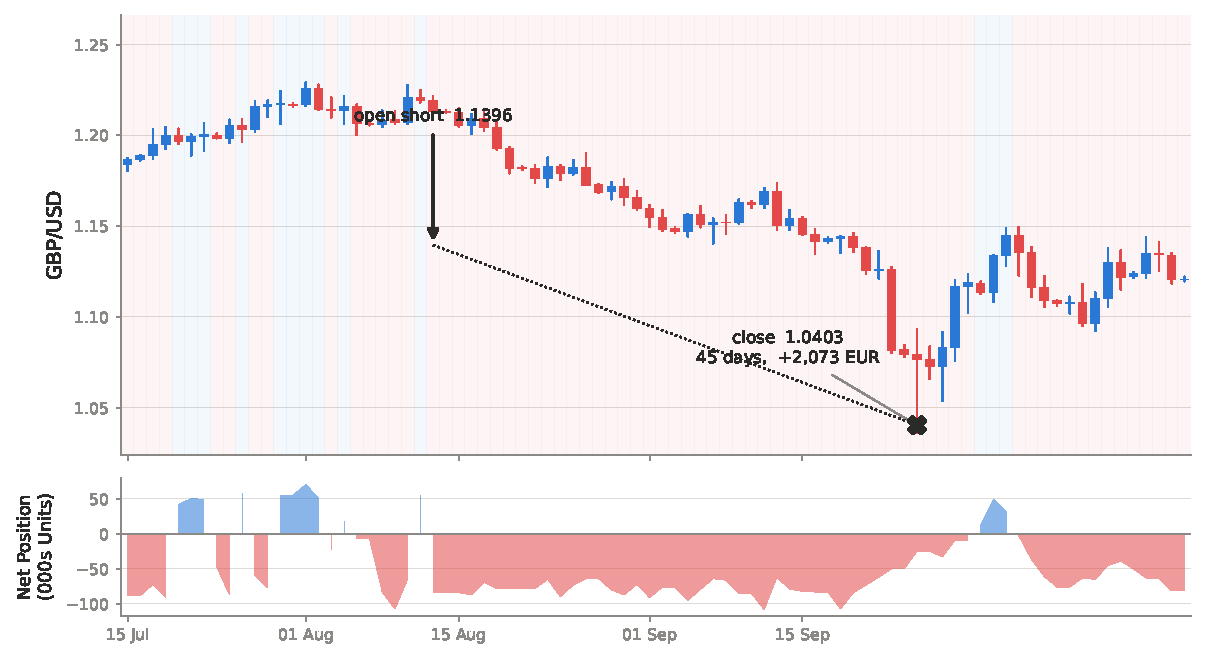
\includegraphics[width=\textwidth]{Images/TrendRide.pdf}
\caption{GBP/USD from mid-July to mid-October 2022. Background shading marks the direction of the net position, red for short and blue for long. The lower panel gives the size of that position. The marked trade is the most profitable single position of the eleven years on this pair.}
\label{Figure:TrendRide}
\end{figure}

The agent was short for almost the whole fall. It held short exposure of between fifty and one hundred thousand units, added to it as the move continued, and reduced it as the price neared the low. The marked position was opened at $1.1396$ on 12 August and closed at $1.0403$ on 26 September, forty-five days later. Its net profit was $2\,073$ euros after costs. It is the largest single position of the eleven years on this pair.

Two details are worth pointing out, because they show judgement and not luck. The agent was briefly long at the end of July, at the local high before the fall began. It was long again in the days right after the bottom. Both times the size was small. It did not hold the short position forever. Once the price recovered above $1.12$ in early October, the position was reduced and then reversed. This is how an agent behaves when it responds to the state it observes, and not when it is fixed on one direction.

\subsection{Holding Periods and Two-Sided Exposure}

\Cref{Tables:Behaviour} gives the trading statistics for each pair, and \Cref{Figure:HoldingBehaviour} shows two of them. Median holding periods go from four days on EUR/USD to nearly thirteen on GBP/USD, and the longest single positions last for months. These agents are swing traders, which hold positions for days, and not scalpers, which trade in and out quickly. This is what the daily decision frequency of \Cref{Section:ExperimentalProcedure} was meant to produce.

\begin{figure}[htb!]
\centering
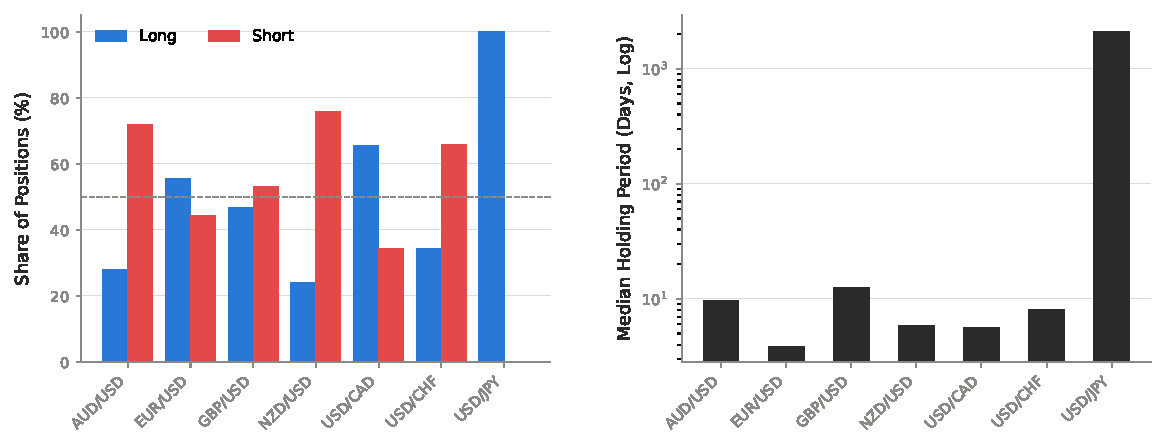
\includegraphics[width=\textwidth]{Images/HoldingBehaviour.pdf}
\caption{Left: the share of positions taken long and short. Right: the median holding period in days, on a logarithmic scale. USD/JPY is long in every position it takes and holds for years, which puts it far outside the range of the other six.}
\label{Figure:HoldingBehaviour}
\end{figure}

The long and short shares differ a lot between pairs, from $24\%$ long on NZD/USD to $66\%$ on USD/CAD. EUR/USD and GBP/USD are close to balanced. None of the six working agents trades only one side. This comes from the design and is not an accident. The eligibility test of \Cref{Section:ExperimentalProcedure} rejected any episode whose weaker side fell below a threshold, so a one-sided policy could not be selected, however profitable it looked. USD/JPY is the exception, at $100\%$ long. It is the exception because none of the $448$ seeds that were tried on that pair could pass that test.

\subsection{Where the Profit Comes From}

One statistic in \Cref{Tables:Behaviour} deserves a closer look. The win rate is the fraction of positions closed at a profit. It lies between $49.8\%$ and $55.0\%$ across the seven pairs. Six of the seven are within three points of a coin toss. USD/CHF, the best model of the seven on every risk measure, has the lowest win rate of all, at $49.8\%$.

So the agents do not make money by being right more often than they are wrong. Their profit comes from what they do with a position once it is open. They hold a larger size when the position moves in their favour than when it does not, and they keep positions that work open longer than positions that do not. A continuous action makes this possible. An agent that can only choose a direction cannot do it. This also explains how USD/CHF can be the strongest model of the seven while being wrong slightly more often than a coin toss. It trades at small size and is patient, and the few positions it holds at a larger size are the ones that worked.

\subsection{What the Trading Costs}

The engine charges the spread quoted at each fill and a real commission schedule. The difference between what the policies earned and what the account kept can therefore be measured, and does not have to be estimated.

The commission is recorded directly on every trade. The spread is not, because it is paid inside each fill and is not deducted afterwards. A buy is filled at the ask and a sell at the bid, so the cost is already included in the entry and exit prices. It can still be recovered exactly, because the two charges scale in the same way. Commission is charged at $3.5$ points per side, which is seven points for a round turn, that is, one opening and one closing trade. The spread is crossed once per round turn. Both are proportional to the traded volume, and both are converted into the account currency at the same rate. So for any position

\begin{equation}
C_{spread} = \left| C_{commission} \right| \cdot \frac{s}{7}
\label{Equation:SpreadRecovery}
\end{equation}

where $s$ is the spread in points at the moment of the trade. Applying \Cref{Equation:SpreadRecovery} to every position gives \Cref{Tables:Costs}, with $s$ taken from the recorded quotes for the month in which the position was opened.

% !TEX root = ../Main.tex
\begin{table}[htb!]
\centering
\footnotesize
\caption{What the seven agents earned before costs and what they kept, in euros. Cost share is the spread and the commission together, as a fraction of profit before costs. The mean spread column is the commission-weighted average spread paid, in points. It differs from the pair's average spread because it gives weight to the moments when the agent traded.}
\label{Tables:Costs}
\begin{tabular}{@{}lrrrrrr@{}}
\toprule
\textbf{Pair} & \textbf{Before Costs} & \textbf{Spread} & \textbf{Commission} & \textbf{Net} & \textbf{Cost Share} & \textbf{Mean Spread} \\
\midrule
AUD/USD & 11,851 & $-1,162$ & $-2,200$ & 8,488 & 28.4\% & 3.70 pts \\
EUR/USD & 9,372 & $-638$ & $-1,669$ & 7,064 & 24.6\% & 2.68 pts \\
GBP/USD & 19,086 & $-2,456$ & $-3,168$ & 13,462 & 29.5\% & 5.43 pts \\
NZD/USD & 8,552 & $-1,238$ & $-1,424$ & 5,890 & \textbf{31.1\%} & 6.09 pts \\
USD/CAD & 28,272 & $-2,695$ & $-3,432$ & 22,145 & 21.7\% & 5.50 pts \\
USD/CHF & 5,735 & $-148$ & $-130$ & 5,457 & \textbf{4.8\%} & 7.93 pts \\
USD/JPY & 2,172 & $-411$ & $-155$ & 1,606 & 26.1\% & 18.53 pts \\
\midrule
\textbf{Total} & \textbf{85,039} & $\mathbf{-8,748}$ & $\mathbf{-12,179}$ & \textbf{64,112} & \textbf{24.6\%} & --- \\
\bottomrule
\end{tabular}
\end{table}

The seven agents earned $85\,039$ euros before costs and kept $64\,112$. Of the difference, $8\,748$ euros went to the spread and $12\,179$ to commission, so \textbf{costs took $24.6\%$ of trading profit}. Commission is the larger of the two charges here because the account is a raw-spread account. On such an account the spread is narrow by design, and the broker makes its money through the commission instead. On an account with wider spreads and no commission, the same trades would have paid a similar total, split in a different way.

\Cref{Tables:Costs} has no swap column because the swap is zero on every pair. A swap-free account charges no overnight financing, so zero is the exact figure and not an approximation. This matters at these holding periods. Agents that hold positions for a median of four to thirteen days would otherwise pay financing on several hundred nights each.

The differences between pairs are large, and they follow turnover almost exactly. USD/CHF takes $220$ positions and gives up $4.8\%$ of its profit before costs, so it keeps more than nineteen euros in every twenty. NZD/USD gives up $31.1\%$ and GBP/USD $29.5\%$. A policy of the same quality therefore gives very different net results at different trading frequencies. This is why the selection criteria of \Cref{Section:ExperimentalProcedure} reward long holding periods directly, instead of relying on the return figure to include this effect. It is also why the rebalance threshold of \Cref{Equation:Hysteresis} contributes as much as \Cref{Tables:Deployment} shows.

One consequence matters for how the rest of this chapter should be read. Every return quoted in this work is net of both charges. A study that tested the same policies on bar closes with no spread and no commission would have reported the before-costs column of \Cref{Tables:Costs}. That column is a third larger, and it describes a strategy that no account could have traded.

Recovering the spread through \Cref{Equation:SpreadRecovery} works, but it is indirect and it needs a commission that is not zero. The engine computes the spread charge internally when it opens a position. It does not yet write this charge to the exported trade record as a separate field. Recording it there, next to commission and swap, is a simple improvement and is noted in \Cref{Section:FutureWork}.

% !TEX root = ../../Main.tex
\section{Path Robustness}
\label{Section:PathRobustness}

Each pair was evaluated from the five starting balances described in \Cref{Section:EvaluationProtocol}. The result is the same in every case: all seven pairs are profitable from all five entry points, thirty-five runs in total, with no exceptions. \Cref{Tables:PathRobustness} gives the individual figures.

% !TEX root = ../Main.tex
\begin{table}[htb!]
\centering
\footnotesize
\caption{Total return from each of the five starting balances, in euros. All thirty-five runs are profitable. Because broker volumes are discrete, a different opening balance rounds positions differently and produces a genuinely different sequence of trades rather than a rescaled copy of the same one.}
\label{Tables:PathRobustness}
\begin{tabular}{@{}lrrrrrrrr@{}}
\toprule
\textbf{Pair} & \textbf{9,900} & \textbf{10,000} & \textbf{10,050} & \textbf{10,100} & \textbf{10,200} & \textbf{Mean} & \textbf{SD} & \textbf{Relative SD} \\
\midrule
AUD/USD & 94.2\% & 87.2\% & 117.1\% & 108.3\% & 105.7\% & 102.5\% & 10.58 & 10.3\% \\
EUR/USD & 69.5\% & 70.6\% & 76.5\% & 77.8\% & 75.1\% & 73.9\% & 3.27 & 4.4\% \\
GBP/USD & 126.5\% & 129.1\% & 127.9\% & 122.0\% & 115.1\% & 124.1\% & 5.11 & \textbf{4.1\%} \\
NZD/USD & 61.7\% & 60.0\% & 54.4\% & 53.7\% & 52.1\% & 56.4\% & 3.76 & 6.7\% \\
USD/CAD & 230.4\% & 221.0\% & 218.5\% & 216.9\% & 246.0\% & 226.6\% & 10.81 & 4.8\% \\
USD/CHF & 56.4\% & 54.8\% & 43.4\% & 52.6\% & 45.5\% & 50.6\% & 5.16 & 10.2\% \\
USD/JPY & 15.9\% & 16.2\% & 16.4\% & 15.7\% & 14.5\% & 15.7\% & 0.69 & 4.4\% \\
\bottomrule
\end{tabular}
\end{table}

The reason this test is worth running is not obvious, so it is worth setting out. A change of one hundred euros in the opening balance looks like a change of scale, and if position sizes were continuous it would be exactly that: every trade would be one percent larger, the equity curve would be a scaled copy, and the percentage return would be identical. Sizes are not continuous. A broker accepts volume in discrete steps, so the reference volume of \Cref{Equation:PositionSizing} is rounded before an order is sent. A slightly larger balance can round a position up where a smaller one rounds it down, which changes the equity available for the next decision, which changes the size of the next position, and so on. Two runs differing only in their opening balance are therefore not the same run rescaled; after a few dozen trades they hold different positions at different times.

That the seven pairs remain profitable across all five paths, with returns clustered rather than scattered, says the results do not depend on one particular sequence of roundings. The relative standard deviation, the standard deviation divided by the mean, sits between $4.1\%$ and $10.3\%$. GBP/USD is the tightest at $4.1\%$ despite being the most active model, and AUD/USD the widest at $10.3\%$.

Two observations follow from the spread of the individual figures. The pairs with the widest relative spread, AUD/USD at $10.3\%$ and USD/CHF at $10.2\%$, are not the pairs with the largest returns; dispersion tracks how close the agent's typical position size sits to a rounding boundary rather than how much it makes. And no pair has a path that turns a profit into a loss, or even into a materially different conclusion: the worst path on USD/CAD still returns $+216.9\%$ and the best on USD/JPY still returns $+16.4\%$, so the ranking between pairs is stable across all five.

What this protocol does not measure should be stated as clearly as what it does. It varies the entry path, not the training run. Each published model is one seed drawn from a pool of between $128$ and $256$, and the variation across that pool is a different and larger source of uncertainty, addressed in \Cref{Section:StatisticalScreening} and again in \Cref{Section:OutOfSample}. A result can be perfectly stable across entry paths and still be the product of a fortunate draw.

% !TEX root = ../../Main.tex
\section{Alpha and Beta Decomposition}
\label{Section:AlphaBeta}

A currency pair moves on its own. An agent that is long a pair that happens to rise will show a profit that has nothing to do with the policy it learned. The same is true for an agent that is short a pair that happens to fall. Total return cannot separate this profit from the profit of the policy. The results are therefore decomposed into the part explained by the market and the part that is not.

For each pair, the yearly return of the model is regressed on the yearly move of the pair itself, over the eleven years from 2015 to 2025. With $r_i$ the model return in year $i$ and $m_i$ the market move in the same year, ordinary least squares gives

\begin{equation}
\beta = \frac{\sum_i (m_i - \bar{m})(r_i - \bar{r})}{\sum_i (m_i - \bar{m})^2}, \qquad \alpha = \bar{r} - \beta \bar{m}
\label{Equation:AlphaBeta}
\end{equation}

$\beta$ measures the model's exposure to the market's movement. $\alpha$ is the average yearly return that is left once that exposure is removed. The mean return then splits into an active part and a passive part:

\begin{equation}
\bar{r} = \underbrace{\alpha}_{\text{policy}} + \underbrace{\beta \bar{m}}_{\text{market exposure}}
\label{Equation:AlphaDecomposition}
\end{equation}

Yearly returns are used instead of daily returns for a specific reason. The agents hold positions for days to weeks and act once a day. A daily regression would therefore measure how the model tracks the market within a holding period. It would not measure whether the model chose the right direction over the horizon it trades. Eleven yearly observations are a small sample, and each regression coefficient has a large uncertainty. The decomposition is good enough to sort the pairs into groups, but it does not give a precise value for any one of them.

\Cref{Tables:AlphaBeta} gives both terms. Six of the seven pairs have positive alpha, and the seven fall into three clear groups.

% !TEX root = ../Main.tex
\begin{table}[htb!]
\centering
\footnotesize
\caption{Decomposition of \Cref{Equation:AlphaDecomposition}, from the yearly regression of \Cref{Equation:AlphaBeta} over 2015 to 2025. Alpha is the return attributable to the policy, and the beta return is the part explained by the pair's own movement. The two add up to the mean yearly return.}
\label{Tables:AlphaBeta}
\begin{tabular}{@{}lrrrrl@{}}
\toprule
\textbf{Pair} & \textbf{Beta} & \textbf{Alpha (\%/yr)} & \textbf{Beta Return (\%/yr)} & \textbf{Mean (\%/yr)} & \textbf{Reading} \\
\midrule
AUD/USD & $-2.013$ & $+4.96$ & $+3.22$ & $+8.18$ & Policy plus leveraged trend \\
EUR/USD & $+0.266$ & $+6.62$ & $+0.01$ & $+6.63$ & Policy, no market exposure \\
GBP/USD & $-0.054$ & $+11.64$ & $+0.06$ & $+11.70$ & Policy, no market exposure \\
NZD/USD & $-0.708$ & $+2.79$ & $+1.83$ & $+4.62$ & Policy plus leveraged trend \\
USD/CAD & $+2.393$ & $+10.02$ & $+4.21$ & $+14.23$ & Policy plus leveraged trend \\
USD/CHF & $-0.082$ & $+3.91$ & $+0.16$ & $+4.07$ & Policy, no market exposure \\
USD/JPY & $+1.012$ & $-1.08$ & $+2.64$ & $+1.57$ & No policy; the model follows the market \\
\bottomrule
\end{tabular}
\end{table}

\textbf{Three pairs have almost no market exposure.} GBP/USD, EUR/USD and USD/CHF have betas of $-0.054$, $+0.266$ and $-0.082$. Their market exposure adds $0.06$, $0.01$ and $0.16$ percentage points per year to their returns. For GBP/USD, $11.64$ of its $11.70$ points per year come from the policy. These results would hold up if the market changed direction, because they hardly depend on the direction of the market.

\textbf{Three pairs combine policy with leveraged exposure.} USD/CAD at $+2.393$, AUD/USD at $-2.013$ and NZD/USD at $-0.708$ all have a large exposure to their market, and two of them are leveraged more than two to one. Their alpha is positive in every case, so the policy adds skill on top. But between a fifth and two fifths of what they earned came from the market moving in the direction of their exposure. USD/CAD is the clearest example: $4.21$ of its $14.23$ points per year came from the pair rising while the agent was net long. If the Canadian Dollar had become stronger over the decade instead, that component would have been a loss of similar size, and the reported $+226.6\%$ would look very different.

\Cref{Figure:AlphaBeta} plots the seven together, and the three groups are clearly separate.

\textbf{One pair has no policy at all.} USD/JPY has a beta of $+1.012$ and a correlation of $+0.946$ with its own market, and its alpha is $-1.08\%$ per year, the only negative figure in the table. It is examined in \Cref{Section:NegativeResult}.

\begin{figure}[htb!]
\centering
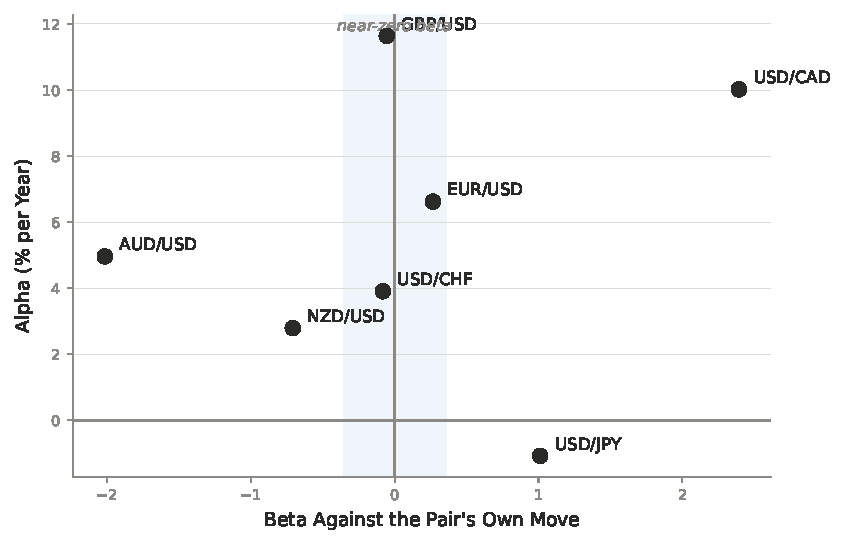
\includegraphics[width=0.82\textwidth]{Images/AlphaBeta.pdf}
\caption{Alpha against beta for the seven agents. Points inside the shaded band have almost no market exposure, so their return is attributable to the policy. USD/JPY sits at a beta of one with negative alpha. This is the pattern of a model that has copied its own market.}
\label{Figure:AlphaBeta}
\end{figure}

The method was checked before it was used. The same regression, run on the model of the previous campaign, reproduces its recorded figures exactly: a correlation of $+0.115$, a beta of $+0.130$ and an alpha of $+3.11\%$ per year. This confirms that the decomposition here is computed in the same way as the one it is compared with.

This decomposition is given priority over total return, for a reason that affects how the whole chapter should be read. The model to publish was chosen from a pool of candidates, and any measure used to make that choice is inflated by it. Return is such a measure. Beta is not. Beta describes how a policy behaves against its market. Selection can give a model a high return by luck, but it cannot give it a low beta in the same way. A large alpha with a beta near zero is therefore a stronger claim than a large return, and it is the claim this work puts first.

% !TEX root = ../../Main.tex
\section{Statistical Screening and the Rejected Candidates}
\label{Section:StatisticalScreening}

Every published model had to pass a test against a null built from the model itself. The model's own sequence of positions is rotated in time. The rotated sequence holds the same positions for the same durations, but at the wrong moments. Its regime score is therefore the score that the model's holding structure earns by luck alone. The published model must beat that score.

The null must be computed for each model and cannot be a fixed number. Across the seven pairs it goes from $48.21$ on GBP/USD to $69.82$ on NZD/USD. A fixed threshold of, say, $55$ would be below chance on one pair and well above it on another. It would accept noise in one market and reject skill in another. This was found by trying a fixed threshold first.

The screening gave a result that changes how the whole campaign should be read. \textbf{On every one of the seven pairs, the candidate with the highest return failed the test.} \Cref{Tables:BetaTraps} lists the strongest cases. A portfolio built by ranking candidates on return would have chosen models that return roughly $+250\%$ on average. Almost all of that return is market exposure, not policy.

% !TEX root = ../Main.tex
\begin{table}[htb!]
\centering
\footnotesize
\caption{Candidates rejected by the screening of \Cref{Section:StatisticalScreening}. On every pair, the candidate with the highest return failed. Ranking on return alone would have chosen these models over the ones published. They show roughly five times the return on paper, but almost none of the measurable skill.}
\label{Tables:BetaTraps}
\begin{tabularx}{\textwidth}{@{}lrrX@{}}
\toprule
\textbf{Pair} & \textbf{Return} & \textbf{$p$-value} & \textbf{Why it was rejected} \\
\midrule
AUD/USD & $+246.8\%$ & $0.146$ & Failed the screen \\
AUD/USD & $+142.6\%$ & $0.987$ & Published during the campaign, then withdrawn when the test was run \\
EUR/USD & $+141.6\%$ & --- & One-sided: long for $86\%$ of the window \\
GBP/USD & $+259.8\%$ & $0.163$ & Failed the screen \\
NZD/USD & $+253.9\%$ & $0.258$ & Failed the screen \\
USD/CHF & $+463.9\%$ & $0.973$ & Positions timed no better than the same positions shuffled; followed the franc trend \\
USD/CHF & $+341.3\%$ & $0.865$ & As above \\
\bottomrule
\end{tabularx}
\end{table}

The USD/CHF case is the clearest. A candidate that returned $+463.94\%$, more than nine times the published model, has a permutation $p$-value of $0.973$. Its positions are timed no better than the same positions shuffled. Its return came from following the trend of the franc. The published model returns a ninth of that, and it is the one with measurable skill.

Two cases are reported because they are uncomfortable. An AUD/USD candidate that returned $+142.55\%$ was published during the campaign. It was withdrawn when its $p$-value came out at $0.987$. On EUR/USD, the model in place at the time won on four of six metrics, including return, Sharpe, Sortino and drawdown. It was still replaced, because it lost on the one measure that decides whether a result is real.

This screening has limits, and they should be stated. Each published model was chosen from between $128$ and $256$ candidates, so a $p$-value near $0.05$ is close to what that many draws give by chance. Under a strict multiple-testing correction, only USD/CAD and GBP/USD, both at $0.0015$, would clearly pass. The permutation test is therefore used here as a screen that rejects bad models, which it clearly did. It is not used as a claim that the remaining models are statistically significant.

% !TEX root = ../../Main.tex
\section{Out-of-Sample Behaviour: The Held-Out Year}
\label{Section:OutOfSample}

The split of \Cref{Equation:Split} trains on 2015 to 2023, selects among episodes on 2024, and does not use 2025 at all. Because the trained weights are stored, 2025 can be scored on its own.

\textbf{The result is negative.} \Cref{Tables:TestYear} gives the figures. Five of the seven pairs lose money in 2025. The mean model return is $-6.8\%$, while the mean market move would have made money. Only USD/CHF, at $+5.0\%$, and USD/JPY, at $+0.6\%$, are positive.

% !TEX root = ../Main.tex
\begin{table}[htb!]
\centering
\footnotesize
\caption{The held-out year against the validation year and the full window. 2025 was seen by no part of the training or selection procedure; 2024 was used to choose which episode's weights were kept. The last column is the move of the pair itself in 2025.}
\label{Tables:TestYear}
\begin{tabular}{@{}lrrrr@{}}
\toprule
\textbf{Pair} & \textbf{2025 (Test)} & \textbf{2024 (Validation)} & \textbf{Full Window} & \textbf{2025 Market} \\
\midrule
AUD/USD & $-11.7\%$ & $+72.4\%$ & $+102.5\%$ & $+7.6\%$ \\
EUR/USD & $-1.2\%$ & $-5.9\%$ & $+73.9\%$ & $+13.5\%$ \\
GBP/USD & $-22.9\%$ & $-3.6\%$ & $+124.1\%$ & $+7.6\%$ \\
NZD/USD & $-5.0\%$ & $+11.0\%$ & $+56.4\%$ & $+2.8\%$ \\
USD/CAD & $-13.4\%$ & $+28.8\%$ & $+226.6\%$ & $-4.6\%$ \\
USD/CHF & $\mathbf{+5.0\%}$ & $+3.7\%$ & $+50.6\%$ & $-12.8\%$ \\
USD/JPY & $+0.6\%$ & $+7.6\%$ & $+15.7\%$ & $-0.7\%$ \\
\midrule
\textbf{Portfolio} & $\mathbf{-9.8\%}$ & --- & $+91.3\%$ & --- \\
\bottomrule
\end{tabular}
\end{table}

The comparison with 2024 is the important part, and \Cref{Figure:YearlyExcess} shows it directly. 2024 is the best year in the whole sample, with a mean excess return of $+16.4$ percentage points over the benchmark. 2025 is the worst, at $-8.7$. The difference between the two years is that 2024 was used to decide which episode's weights were kept, and 2025 was not used for anything. This gap is the measured effect of selection. It is the reason the full-window figures in \Cref{Tables:PairResults} are called an in-sample result throughout this thesis.

\begin{figure}[htb!]
\centering
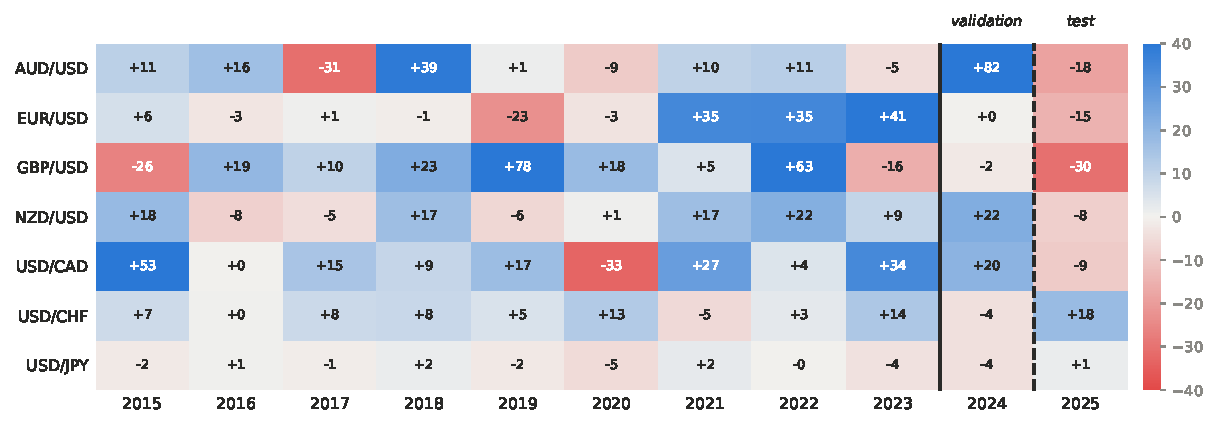
\includegraphics[width=\textwidth]{Images/YearlyExcess.pdf}
\caption{Yearly return of each agent minus the return of buying and holding the same pair, in percentage points. Blue marks outperformance of the benchmark. The solid line marks the end of the training data and the dashed line the end of the validation year, so only the last column was not seen by any part of the procedure.}
\label{Figure:YearlyExcess}
\end{figure}

There is a market explanation for the direction of the 2025 result. It is worth giving because it leads to a useful conclusion. In 2025 there was a broad dollar reversal. EUR/USD rose $13.5\%$, its largest yearly move in the eleven years, and the dollar became weaker against five of the seven pairs. The agents were trained on a decade in which the dollar mostly became stronger, and six of the seven were positioned for that. The seventh, USD/CHF, is the least directional model of the seven. It holds the fewest positions and has the lowest beta, and it is the one that made money. This agrees with the rest of the evidence and is not a coincidence. The model that depends least on the direction of the market is the one that held up when that direction changed.

The individual results should be read, and not only their average, because the models do not fail in the same way. GBP/USD is the worst, at $-22.9\%$. It is the most aggressive model of the seven. It trades near full size and has the deepest drawdown over the full window, so a year that goes against it costs a lot. USD/CAD loses $13.4\%$ and AUD/USD $11.7\%$. Both are leveraged-exposure models of \Cref{Section:AlphaBeta}, so a reversal in the direction of their beta is exactly the event that hurts them. EUR/USD loses only $1.2\%$, although the pair moved $13.5\%$. This agrees with its beta near zero: it did not take part in the reversal in either direction.

The two models that held up are the two that held the least. USD/CHF returned $+5.0\%$ while its pair fell $12.8\%$. That is an excess return of $17.8$ percentage points, and its best year against the benchmark in the whole sample. USD/JPY returned $+0.6\%$. This is not skill. It only means that the model was not exposed to the pairs that moved. Together, the two show the pattern: the models that depended least on the direction of the market were the ones that held up when that direction changed.

One year is a small sample, and no conclusion should be drawn from it beyond the obvious one. The held-out year limits what can be claimed, but it is not a final judgement on the design. The design kept trading in a sensible way on data it had never seen. It lost money doing so, in a year whose direction was not in its training data.

% !TEX root = ../../Main.tex
\section{A Negative Result: USD/JPY}
\label{Section:NegativeResult}

USD/JPY did not work, and the reason is known.

The numbers show that the model behaves like the market. Its correlation with the pair's yearly move is $+0.946$ and its beta is $+1.012$, so its exposure to the pair is almost exactly one for one. Its alpha is $-1.07\%$ per year. It returns $+15.7\%$ over the eleven years, against roughly $+25\%$ for simply buying and holding the pair. It therefore underperforms a benchmark that costs nothing to run. The model is long at every point in the window.

The cause is in the data. USD/JPY rose from roughly $120$ to $150$ over the period, and the move was concentrated and mostly in one direction. On such a series, holding a long position is close to optimal, and any change from it is punished. The reward signal therefore gives no gradient towards changing the exposure, and the agent settles on the simplest policy that follows the trend. Over the same period the other six majors mean-revert often enough that trading both sides is rewarded, and their agents learned to do it.

This was not assumed. It was tested. Across seven configurations and $448$ seeds, every run converged to a directional policy at full size. One augmentation shows the agent mirrored price series, and it was meant to remove exactly this bias. Raising it made the resulting policies more binary, not less.

The result is reported because it is informative. It shows the limit of the method. This design learns to time its exposure in markets that turn. On a market that does not turn, it ends up just holding the trend, and it pays trading costs to do so. A reader who is deciding whether to use the approach elsewhere needs to know this limit more than they need a seventh success.

% !TEX root = ../../Main.tex
\section{Portfolio: The Seven Models Combined}
\label{Section:Portfolio}

A trader would not run just one of these agents. They would run all seven. This is a different question from how each agent does alone. For a portfolio, what matters is not only what each component returns, but also whether the components lose money at the same time.

The seven published models are combined by giving each one a seventh of the capital at the start of the window, with no rebalancing afterwards. With $E_p(t)$ the equity of pair $p$ at time $t$, the portfolio is

\begin{equation}
V(t) = \frac{1}{7} \sum_{p} \frac{E_p(t)}{E_p(0)}
\label{Equation:Portfolio}
\end{equation}

By construction, the total return of such a portfolio is the mean of its components. The interesting part is therefore the risk, and not the return. \Cref{Tables:Portfolio} compares the portfolio with the average of the seven pairs taken separately.

% !TEX root = ../Main.tex
\begin{table}[htb!]
\centering
\footnotesize
\caption{The equal-weight portfolio of \Cref{Equation:Portfolio} against the average of its seven components. Return is the same by construction, so the whole effect is on risk.}
\label{Tables:Portfolio}
\begin{tabular}{@{}lrrl@{}}
\toprule
\textbf{Measure} & \textbf{Portfolio} & \textbf{Mean of the seven} & \textbf{Effect} \\
\midrule
Total return & $+91.3\%$ & $+91.3\%$ & Equal by construction \\
Annualised return & $+6.07\%$ & $+6.07\%$ & Equal by construction \\
\addlinespace
Maximum drawdown & $\mathbf{15.9\%}$ & $34.5\%$ & More than halved \\
Sharpe ratio & $\mathbf{0.632}$ & $0.451$ & Above all but USD/CHF \\
Sortino ratio & $0.906$ & $0.685$ & Improved \\
Calmar ratio & $0.381$ & $0.194$ & Nearly doubled \\
Sterling ratio & $1.059$ & $0.670$ & Improved \\
\addlinespace
Mean correlation & \multicolumn{2}{c}{$+0.062$ across all 21 pairings} & Close to independent \\
\bottomrule
\end{tabular}
\end{table}

\Cref{Figure:PortfolioEquity} plots the portfolio against its components. The maximum drawdown falls from an average of $34.5\%$ to $15.9\%$. The Sharpe ratio rises from an average of $0.451$ to $0.632$, which is above every single pair except USD/CHF. The portfolio gives the same return with less than half the worst loss.

\begin{figure}[htb!]
\centering
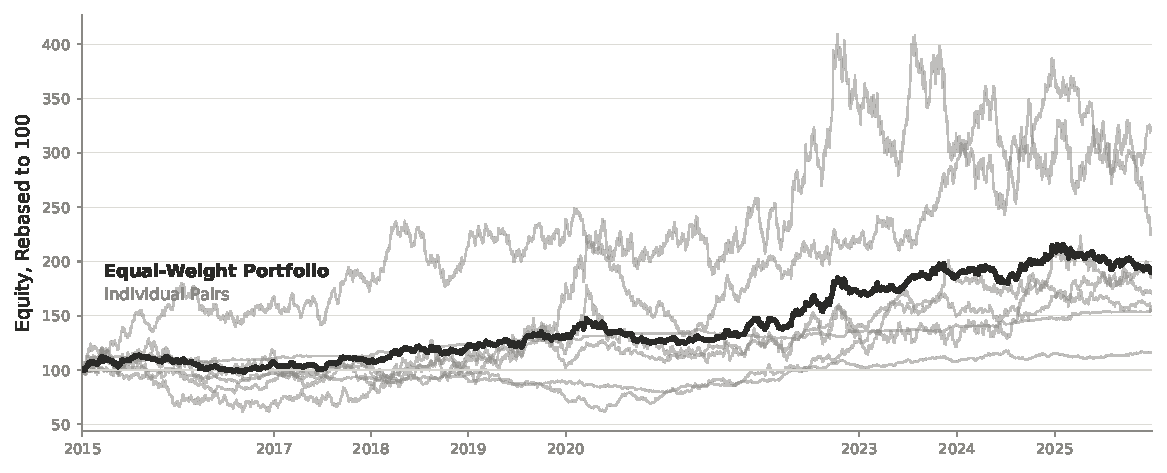
\includegraphics[width=\textwidth]{Images/PortfolioEquity.pdf}
\caption{The equal-weight portfolio against its seven components, all rebased to 100. The portfolio is smoother than any component because the components do not fall together.}
\label{Figure:PortfolioEquity}
\end{figure}

\Cref{Figure:Correlation} shows the reason. The mean correlation between the daily returns of any two of the seven models is $+0.062$, and no pair of models is above $+0.46$. Three pairings are negative. The seven agents were trained by the same procedure on seven instruments that are themselves correlated, since all of them have the US Dollar on one side. Even so, their profits and losses come at different times. This follows from the design. Each agent learned the timing of its own market, so the agents share a method but not a position.

\begin{figure}[htb!]
\centering
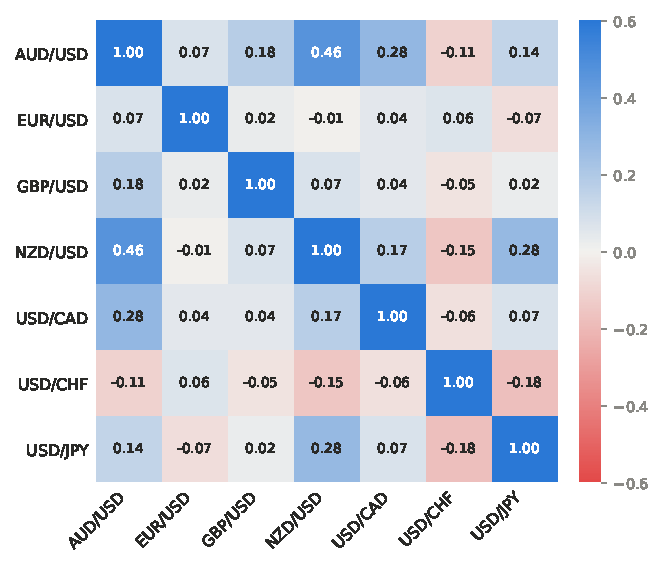
\includegraphics[width=0.68\textwidth]{Images/Correlation.pdf}
\caption{Correlation between the daily returns of the seven agents over the evaluation window. The mean of the off-diagonal entries is $+0.062$.}
\label{Figure:Correlation}
\end{figure}

\subsection{Does the Result Depend on the Position Sizes?}

As \Cref{Section:EvaluationProtocol} states, the seven models do not all run at the same position size. The portfolio above is therefore the combination as published, and it is not built on a common risk level. It is fair to ask whether this choice produces the result. The question can be checked directly.

Position size is proportional to the account balance. Multiplying the risk fraction by a constant therefore multiplies every position, and so every per-step return, by the same constant. A common-risk version can be built by rescaling each component's returns to the level it would have run at, and compounding them again. This ignores the rounding of volumes to the broker's step and any margin limit. It is an approximation and not a new run, but it is close enough to answer the question. \Cref{Tables:CommonRisk} gives both versions.

% !TEX root = ../Main.tex
\begin{table}[htb!]
\centering
\footnotesize
\caption{The equal-weight portfolio as published, against a version in which every component runs at a common risk level. The common-risk version is built by rescaling each component's per-step returns. This is exact for a strategy whose position size is proportional to balance, but it ignores volume rounding. The two differ little, so the diversification result does not depend on how positions are sized.}
\label{Tables:CommonRisk}
\begin{tabular}{@{}lrrr@{}}
\toprule
\textbf{Measure} & \textbf{As Published} & \textbf{Common Risk} & \textbf{Difference} \\
\midrule
Total return & $+91.3\%$ & $+91.6\%$ & $+0.3$ pp \\
Annualised return & $+6.07\%$ & $+6.09\%$ & $+0.02$ pp \\
Sharpe ratio & $0.632$ & $0.608$ & $-0.024$ \\
Sortino ratio & $0.906$ & $0.866$ & $-0.040$ \\
Calmar ratio & $0.381$ & $0.320$ & $-0.061$ \\
Maximum drawdown & $15.9\%$ & $19.0\%$ & $+3.1$ pp \\
\bottomrule
\end{tabular}
\end{table}

The two portfolios are almost the same. Total return moves from $+91.3\%$ to $+91.6\%$, the Sharpe ratio from $0.632$ to $0.608$, and the maximum drawdown from $15.9\%$ to $19.0\%$. The common-risk version is slightly worse on risk, as expected. Putting USD/JPY at the same risk level as the others makes its positions five times larger and takes its own maximum drawdown to roughly $80\%$. At a seventh of the capital, the portfolio absorbs even that. The conclusion of this section therefore does not depend on how the positions are sized. It depends on the correlation structure of the models, which sizing does not change.

Two limits apply to this result. As \Cref{Section:EvaluationProtocol} states, the components do not all run at the same position size. The portfolio is therefore the combination as published, and not a risk-parity allocation. Making the sizes equal would change the weights, but not the correlation structure that produces the benefit. Also, the portfolio shares the weakness of its components. In the held-out year of \Cref{Section:OutOfSample} it returns $-9.8\%$, better than five of the seven pairs and worse than two. This is what an average should do when most of its components fall together for a shared reason.

Two results matter most. First, six of the seven agents produced positive alpha against their own market. Three of those did so with a market sensitivity close to zero, and this is what separates a trading strategy from leveraged market exposure. Second, the seven agents combined behave better than any of them alone, because their returns are close to uncorrelated.

On the other hand, the held-out year is negative, and the selection is not corrected for multiple testing. \Cref{Chapter:Conclusion} sets out what these two facts allow this work to claim and what they do not.
\cleardoublepage
%
% !TEX root = ../../Main.tex
\fancychapter{Conclusion}
\label{Chapter:Conclusion}

The aim of this work was to find out whether one deep reinforcement learning design gives a profitable policy with controlled risk on all seven major currency pairs. The design was trained separately for each instrument and was otherwise not changed. The evaluation charged the same costs that a real account charges.

The answer is yes, but with conditions. These conditions are as much a part of the result as the answer itself.

% !TEX root = ../../Main.tex
\section{Summary}
\label{Section:Summary}

This work built three things and answered one question.

The first is a trading framework. In it, one strategy implementation runs in three places: an offline backtest over stored quotes, the cTrader backtesting tab, and a live account. Its execution engine reproduces the platform's own results byte for byte on six reference configurations. It also goes further than the platform. It steps through every tick instead of only the bar closes, and it charges the spread recorded at the moment of each trade. The framework reads from a market database of $1.66$ billion quotes for the seven pairs, which takes up $295$ GB. Every bar series used in this work is built from this database.

The second is an agent. It observes thirty-eight dimensionless values, built from sixteen technical indicators. It outputs one continuous action that sets both the direction and the size of its position at the same time. Six changes to the published algorithm were needed to make it train on this problem, and two of them matter most. The first is a scale-sensitive reward. A scale-invariant reward gives no gradient towards holding a position large enough to matter. The second is a penalty on the actor's pre-activation. Without it, the policy saturates at $+1$ or $-1$ and collapses to a constant action.

The third is a selection procedure. First, gates reject candidates with degenerate policies, such as those that hardly trade or keep to one side of the market. Next, each candidate is tested against a null built from itself, by rotating the model's own sequence of positions in time. Last, the candidates are ranked by a composite score in which return is one of nine parts. The procedure was not designed to be elegant. It was built because ranking on return does not work, and \Cref{Section:StatisticalScreening} shows this with measured results.

The answer to the question is as follows. All seven agents are profitable over the eleven-year window, from each of the five starting balances. Their total returns range from $+15.7\%$ to $+226.6\%$ net of the spread and commission of a swap-free raw-spread account. Six of the seven have a positive alpha when their return is decomposed against their own market. Three of these six do this with almost no market exposure. The seventh, USD/JPY, only follows its market. It is reported as a failure, together with a diagnosis of its cause. An equal-weight portfolio of the seven lowers the maximum drawdown from an average of $34.5\%$ to $15.9\%$ and raises the Sharpe ratio to $0.632$. This happens because the agents are close to uncorrelated with one another.

Two findings lie behind these numbers. They are more likely than the numbers themselves to carry over to other problems. First, the agents really use the continuous action. The mean absolute action ranges from $0.09$ to $0.98$ across the pairs, and saturation is below one percent on every pair. So the agents learned to size their positions, and they do not just switch between the two extremes. Second, win rates lie between $49.8\%$ and $55.0\%$, and the strongest model in the set has the lowest win rate. So the profit does not come from being right more often. It comes from what the agents do with a position once it is open. A continuous action makes this possible and a discrete action does not.

% !TEX root = ../../Main.tex
\section{Limitations}
\label{Section:Limitations}

The most important limitation comes first, because it puts a limit on everything else. The performance figures in \Cref{Chapter:ExperimentalResults} are measured over a window that includes the years the agents were trained on. The procedure does keep one year out of training and out of the choice among an agent's own episodes. But the choice of which trained agent to publish was made on the full window, so the headline returns are an in-sample result. On the one year that no part of the procedure saw, the models lost money. The portfolio returned $-9.8\%$ in 2025, and five of the seven pairs were negative. That year had a broad dollar reversal, and the training decade had none. The one model that held up is the least directional model in the set. However, a single year is a small sample, and no stronger conclusion should be drawn from it in either direction.

There is a second way in which the selection is not corrected. Each published model was chosen from between $128$ and $256$ candidates. With that many draws, a permutation $p$-value near $0.05$ is close to what chance alone produces. For this reason, the screening is reported as a filter that was shown to reject bad models. It is not reported as a claim that the models that passed are statistically significant. Under a strict correction, only USD/CAD and GBP/USD would clearly pass.

Three smaller limitations should also be recorded. First, the position size was chosen for each pair after the results were seen. It scales every trade and does not change the policy that makes the trades. Still, it is a parameter fitted on the same data as everything else. Second, training cannot be reproduced across environments. It is bit-exact within one installation on a single thread, but a different version of a numerical library changes the outcome. So the delivered models are archived artifacts whose replay has been verified. They are not a recipe that can produce the same models again. Third, two weeks of January 2016 are missing from all seven pairs, for reasons on the broker's side. The gap is the same for all pairs and lies outside the evaluation window, so it does not bias any comparison in this work.

Finally, the tests cover a narrower scope than the method itself. They use seven instruments from one asset class, one eleven-year period, one decision frequency and one cost model. This is only one case out of many possible ones. Nothing in this work shows that the design carries over to other markets, other periods or other holding horizons. The USD/JPY result shows that it does not carry over to every instrument, even among the seven.

% !TEX root = ../../Main.tex
\section{Future Work}
\label{Section:FutureWork}

The limitations above set the order of the future work. The most useful next step is the one that would most change the value of the results.

The first step is a true held-out evaluation. Training would end before the reporting period starts. The choice among candidates would use only data from before that point. The reported figures would then be an out-of-sample estimate. They would no longer describe the same window on which the models were chosen. Of all possible changes, this one would do the most to make the claims stronger. The framework already supports it. It needs a campaign run under this stricter protocol, and it needs no new features in the framework.

The second step follows from the first. The procedure used here splits the window only once. A walk-forward scheme with several folds would train each fold on the data before it and evaluate it on the data after it. This would give an out-of-sample record for the whole period, and not just for one year. The learned weights could also be carried from one fold into the next, instead of starting each fold from a new initialisation. This would test whether an agent adapts as the market changes. The framework supports this, but it was not used in this campaign.

The third step is to report how much the results vary between training runs. The path-robustness protocol used here changes the starting balance. This measures how sensitive a result is to the entry path, but not how sensitive it is to the training itself. The next step would report the distribution of outcomes across the whole pool of candidates, and where the published model falls within it. A reader could then see how much of a result comes from the method and how much comes from chance.

Apart from the evaluation, what the agents did suggests three further directions. The portfolio in \Cref{Section:Portfolio} gives the seven agents equal weights. Weighting them by risk, or by their correlation structure, should do better. The seven agents are almost independent of each other, which suggests that the gain would be real. The observation holds thirty-eight values from a single point in time. The natural next step is a recurrent or attention-based encoder that reads a window of past data directly. This was part of the original plan for this work. Last, the framework already runs the same strategy on a live account. A live deployment over a long period would test whether the execution assumptions hold when the orders are real. No backtest can test this.

One improvement to the framework itself should also be noted. The execution engine charges the spread correctly, by filling orders at the ask and at the bid. However, the exported trade record does not show this cost as a separate field. To recover it, the indirect calculation of \Cref{Equation:SpreadRecovery} is needed. If every trade recorded the spread cost next to its commission and swap, the cost decomposition in \Cref{Tables:Costs} could be read directly and would not have to be inferred. It could also be reported for each position, and not only in total.

The USD/JPY result needs a separate note. The current explanation of the failure on this pair is that the price window is monotonic, which means the price moves in one direction only. Such a window gives no gradient towards changing the size of the exposure. It has not been shown that this is the whole explanation. The pair should be studied again once the evaluation protocol above is in place.

Some reported returns suggest that deep reinforcement learning for currency trading is a solved problem. Its out-of-sample record suggests that it leads nowhere. Neither view is correct. This work shows that the main difficulty is not in the learning algorithm. It is in the environment the agent is trained in and in the costs it is charged. Most of all, it is in a careful and strict way of deciding which of many trained models to trust. Six of the seven agents produced returns that still hold after a decomposition into policy and market exposure. For all seven pairs, the candidate that looked best on return did not pass this test.
%
% -----------------------------------------------------------------------------
% Bibliography
\addcontentsline{toc}{chapter}{Bibliography}
\bibliographystyle{IEEEtran}
\normalem
\bibliography{./Bibliography}
\ULforem
%
% -----------------------------------------------------------------------------
% Appendices
\appendix
% !TEX root = ../../Main.tex
\chapter{Technical Indicators}
\label{Appendix:TechnicalIndicators}

% !TEX root = ../Main.tex
\begin{table}[htb!]
\centering
\footnotesize
\caption{Summary of frequently used Trend Technical Indicators \cite{jansen_machine_2020}.}
\label{Tables:TrendIndicators}
\begin{tabularx}{\textwidth}{@{}lXl@{}}
\toprule
\textbf{Indicator Name} & \textbf{Formula} & \textbf{Range} \\
\midrule
Simple Moving Average & $\text{SMA}(N)_t = \frac{1}{N} \sum_{i=1}^{N} \text{Price}_{t-N+i}$ & - \\
\addlinespace
Exponential Moving Average & $\text{EMA}(N)_t = \frac{2}{N+1} \times \text{Price}_t + (1 - \frac{2}{N+1}) \times \text{EMA}(N)_{t-1}$ & - \\
\addlinespace
Weighted Moving Average & $\text{WMA}(N)_t = \frac{2}{N \times (N + 1)} \sum_{i=1}^{N} i \times \text{Price}_{t-N+i}$ & - \\
\addlinespace
Double Exponential Moving Average & $\text{DEMA}(N)_t = 2 \times \text{EMA}(N)_t - \text{EMA}_2(N)_t$ & - \\
\addlinespace
Triple Exponential Moving Average & $\text{TEMA}(N)_t = 3 \times [\text{EMA}(N)_t - \text{EMA}_2(N)_t] + \text{EMA}_3(N)_t$ & - \\
\addlinespace
Hull Moving Average & $\text{HMA}(N)_t = \text{WMA}\left(\sqrt{N}\right)\left[2 \times \text{WMA}\left(\frac{N}{2}\right)_t - \text{WMA}(N)_t\right]$ & - \\
\addlinespace
Triangular Moving Average & $\text{TRIMA}(N)_t = \frac{1}{N} \sum_{i=1}^{N} \text{SMA}(N)_{t-N+i}$ & - \\
\addlinespace
Efficiency Ratio & $\text{ER}(N)_t = \frac{| \text{Price}_t - \text{Price}_{t-N} |}{\sum_{i=1}^{N} | \text{Price}_{t-i+1} - \text{Price}_{t-i} |}$ & [0, 1] \\
\addlinespace
Kaufman Adaptive Moving Average & $\text{KAMA}(N)_t = \text{KAMA}(N)_{t-1} + \text{SC} \times (\text{Price}_t - \text{KAMA}(N)_{t-1})$ & - \\
\addlinespace
& $\text{SC} = [ \text{ER}(N)_t \times (\phi_{\text{short}} - \phi_{\text{long}}) + \phi_{\text{long}} ]^2, \phi_{\text{short}} = \frac{2}{N_{\text{short}} + 1}$, $\phi_{\text{long}} = \frac{2}{N_{\text{long}} + 1}$ & \\
\addlinespace
& where typically $N_{\text{short}} = 2$ and $N_{\text{long}} = 30$ & \\
\bottomrule
\end{tabularx}
\end{table}
% !TEX root = ../Main.tex
\begin{table}[htb!]
\centering
\footnotesize
\caption{Summary of frequently used Momentum Technical Indicators \cite{jansen_machine_2020}.}
\label{Tables:MomentumIndicators}
\begin{tabularx}{\textwidth}{@{}lXl@{}}
\toprule
\textbf{Indicator Name} & \textbf{Formula} & \textbf{Range} \\
\midrule
Price Momentum & $\text{PM}_t = \frac{\text{Price}_t - \text{Price}_{t-1}}{\text{Price}_{t-1}}$ & - \\
\addlinespace
Rate of Change & $\text{ROC}(N)_t = \ln\left(\frac{\text{Price}_t}{\text{Price}_{t-N}}\right)$ & - \\
\addlinespace
Price Acceleration & $\text{PA}_t = \frac{\text{Short Linear Regression Coefficient}}{\text{Long Linear Regression Coefficient}} = \frac{\beta_\text{short}}{\beta_\text{long}}$ & - \\
\addlinespace
Relative Strength Index & $\text{RSI}(N)_t = 100 - \frac{100}{1 + \frac{\text{Average Gain}_t}{\text{Average Loss}_t}}$ & [0, 100] \\
\addlinespace
& $\text{Average Gain}_t = \frac{1}{N}\sum_{i=1}^{N} \max(\text{Price}_i - \text{Price}_{i-1}, 0)$ & \\
\addlinespace
& $\text{Average Loss}_t = \frac{1}{N}\sum_{i=1}^{N} \max(\text{Price}_{i-1} - \text{Price}_i, 0)$ & \\
\addlinespace
Aroon Oscillator & $\text{Aroon}(N)_t = \text{Aroon Up}(N)_t - \text{Aroon Down}(N)_t$ & [-100, 100] \\
\addlinespace
& $\text{Aroon Up}(N)_t = \left( \frac{N - \text{Periods Since Highest High in } N}{N} \right) \times 100$ & \\
\addlinespace
& $\text{Aroon Down}(N)_t = \left( \frac{N - \text{Periods Since Lowest Low in } N}{N} \right) \times 100$ & \\
\addlinespace
Balance of Power & $\text{BOP}_t = \frac{\text{Close}_t - \text{Open}_t}{\text{High}_t - \text{Low}_t}$ & [-1, 1] \\
\addlinespace
Commodity Channel Index & $\text{CCI}(N)_t = \frac{\text{TP}_t - \text{SMA}_\text{TP}(N)_t}{0.015 \times \text{Mean Deviation}(N)_t}$ & - \\
\addlinespace
& $\text{TP}_t = \frac{\text{High}_t + \text{Low}_t + \text{Close}_t}{3}$ & \\
\addlinespace
& $\text{Mean Deviation}(N)_t = \frac{1}{N}\sum_{i=1}^{N} |\text{TP}_i - \text{SMA}_\text{TP}(N)_t|$ & \\
\addlinespace
Moving Average Convergence Divergence & $\text{MACD}_t = \text{EMA}(N_{\text{short}})_t - \text{EMA}(N_{\text{long}})_t $ & - \\
\addlinespace
& where typically $N_{\text{short}} = 12$ and $N_{\text{long}} = 26$ & \\
\addlinespace
Stochastic RSI & $\text{StochRSI}(N)_t = \frac{\text{RSI}(N)_t - \min(\text{RSI}(N))}{\max(\text{RSI}(N)) - \min(\text{RSI}(N))}$ & [0, 1] \\
\addlinespace
Stochastic Oscillator & $\text{Stoch \%K}(N)_t = \frac{\text{Close}_t - \text{LL}(N)_t}{\text{HH}(N)_t - \text{LL}(N)_t} \times 100$ & [0, 100] \\
\addlinespace
& $\text{Stoch \%D}(M)_t = \text{SMA}_{\text{Stoch \%K}(N)}(M)_t$ & [0, 100] \\
\addlinespace
& $\text{HH}(N)_t = \max_{i=t-N+1}^{t}(\text{High}_i)$, $\text{LL}(N)_t = \min_{i=t-N+1}^{t}(\text{Low}_i)$ & \\
\addlinespace
Ultimate Oscillator & $\text{UO}_t = \frac{4 \times \text{Avg}_t(N_1) + 2 \times \text{Avg}_t(N_2) + \text{Avg}_t(N_3)}{4+2+1} \times 100$ & [0, 100] \\
\addlinespace
& $\text{Avg}_t(N) = \frac{\sum_{i=0}^{N-1}\text{BP}_{t-i}}{\sum_{i=0}^{N-1}\text{TR}_{t-i}}$ & \\
\addlinespace
& $\text{BP}_t = \text{Close}_t - \min(\text{Close}_{t-1}, \text{Low}_t)$ & \\
\addlinespace
& $\text{TR}_t = \max(\text{Close}_{t-1}, \text{High}_t) - \min(\text{Close}_{t-1}, \text{Low}_t)$ & \\
\addlinespace
& where typically $N_1 = 7$, $N_2 = 14$, and $N_3 = 28$ & \\
\addlinespace
Williams \%R & $\text{Williams \%R}(N)_t = \frac{\text{HH}(N)_t - \text{Close}_t}{\text{HH}(N)_t - \text{LL}(N)_t} \times -100$ & [-100, 0] \\
\bottomrule
\end{tabularx}
\end{table}
% !TEX root = ../Main.tex
\begin{table}[htb!]
\centering
\footnotesize
\caption{Summary of frequently used Volume Technical Indicators \cite{jansen_machine_2020}.}
\label{Tables:VolumeIndicators}
\begin{tabularx}{\textwidth}{@{}lXl@{}}
\toprule
\textbf{Indicator Name} & \textbf{Formula} & \textbf{Range} \\
\midrule
Chaikin Accumulation/Distribution Line & $\text{AD}_t = \text{AD}_{t-1} + \text{MFV}_t$ & - \\
\addlinespace
& $\text{MFV}_t = \frac{(\text{Close}_t - \text{Low}_t) - (\text{High}_t - \text{Close}_t)}{\text{High}_t - \text{Low}_t} \times \text{Volume}_t$ & \\
\addlinespace
Chaikin Accumulation/Distribution Oscillator & $\text{ADOSC}_t = \text{EMA}_\text{AD}(N_{\text{short}})_t - \text{EMA}_\text{AD}(N_{\text{long}})_t$ & - \\
\addlinespace
& where typically $N_{\text{short}} = 3$ and $N_{\text{long}} = 10$ & \\
\addlinespace
On-Balance Volume & $\text{OBV}_t =
\begin{cases}
\text{OBV}_{t-1} + \text{Volume}_t & \text{if } \text{Price}_t > \text{Price}_{t-1} \\
\text{OBV}_{t-1} - \text{Volume}_t & \text{if } \text{Price}_t < \text{Price}_{t-1} \\
\text{OBV}_{t-1} & \text{otherwise}
\end{cases}$ & - \\
\bottomrule
\end{tabularx}
\end{table}
% !TEX root = ../Main.tex
\begin{table}[htb!]
\centering
\footnotesize
\caption{Summary of frequently used Volatility Technical Indicators \cite{jansen_machine_2020}.}
\label{Tables:VolatilityIndicators}
\begin{tabularx}{\textwidth}{@{}lXl@{}}
\toprule
\textbf{Indicator Name} & \textbf{Formula} & \textbf{Range} \\
\midrule
Standard Deviation & $\text{SD}(N)_t = \sqrt{\frac{1}{N-1} \sum_{i=1}^{N} (\text{Price}_i - \overline{\text{Price}})^2}$ & - \\
\addlinespace
Realised Volatility & $\text{RV}(N)_t = \sqrt{\sigma^2_t}$, where $\sigma^2_t = \alpha \times r_t^2 + (1 - \alpha) \times \sigma^2_{t-1}$, $r_t = \ln\left(\frac{\text{Price}_t}{\text{Price}_{t-1}}\right)$ and $\alpha = \frac{1}{N}$ & - \\
\addlinespace
Bollinger Bands & $\text{Upper BB}(N, k)_t = \text{SMA}(N)_t + k \times \text{SD}(N)_t$ & - \\
\addlinespace
& $\text{Lower BB}(N, k)_t = \text{SMA}(N)_t - k \times \text{SD}(N)_t$ & \\
\addlinespace
& where typically $ k = 2 $& \\
\addlinespace
Average True Range & $\text{ATR}(N)_t = \frac{(N - 1) \times \text{ATR}(N)_{t-1} + \text{TRANGE}_t}{N}$ & - \\
\addlinespace
& $\text{TRANGE}_t = \max(\text{High}_t - \text{Low}_t, |\text{High}_t - \text{Close}_{t-1}|, |\text{Low}_t - \text{Close}_{t-1}|)$ & \\
\addlinespace
Normalised Average True Range & $\text{NATR}(N)_t = \frac{\text{ATR}(N)_t}{\text{Close}_t} \times 100$ & - \\
\addlinespace
Chaikin Volatility Index & $\text{CVI}(N)_t = \frac{\text{EMA}_{HL}(N)_t - \text{EMA}_{HL}(N)_{t-N}}{\text{EMA}_{HL}(N)_{t-N}} \times 100$ & - \\
\addlinespace
& $\text{EMA}_{HL}(N)_t = \text{EMA}(N)$ applied to $(\text{High}_t - \text{Low}_t)$ & \\
\bottomrule
\end{tabularx}
\end{table}
\cleardoublepage
%
% !TEX root = ../../Main.tex
\chapter{Reviewed Articles}
\label{Appendix:ReviewedArticles}

% !TEX root = ../Main.tex
\begin{sidewaystable}
%\begin{landscape}
%\begin{table}[htb!]
\centering
\footnotesize
\caption{Basic features of the related work articles.}
\label{Tables:BasicRelatedWork}
\begin{tabularx}{\linewidth}{@{}ccccccccX@{}}
\toprule
\textbf{Reference} & \textbf{Market} & \textbf{Dataset} & \textbf{Timeframe} & \textbf{Period} & \textbf{NN} & \textbf{RL} & \textbf{DRL} & \textbf{Key Findings} \\
\midrule

\cite{carapuco_reinforcement_2018} & Forex & Raw Ticks & \(\approx\) 2 Hours & 2010 - 2017 & FNN & Critic-Only & DQN & Significantly outperformed the benchmark. \\

\cite{huang_financial_2018} & Forex & OHLCV & 15 Minutes & 2012 - 2017 & RNN (LSTM) & Critic-Only & DRQN & Significantly outperformed the benchmark even with explicit and implicit costs. \\

\cite{rundo_deep_2019} & Forex & OHLCV & Minute & 2004 - 2018 & RNN (LSTM) & Critic-Only & DRQN & Outperformed the benchmark, but with unusually high accuracy and maximum drawdown. \\

\cite{saini_stock_2019} & Stocks & \makecell{OHLCV, \\ News} & Daily & \(\approx\) 5 Months & RNN (LSTM) & Actor-Critic & DDPG & Outperformed the benchmark. News features were important. \\

\cite{gran_deep_2019} & Stocks & OHLCV & Monthly & 2005 - 2019 & FNN & Actor-Critic & DDPG & Outperformed the benchmark even with explicit and implicit costs. \\

\cite{kong_empirical_2023} & Stocks & OHLCV & Daily & 2016 - 2020 & FNN & Actor-Critic & \makecell{DDPG, \\ A2C, PPO} & The ensemble underperformed the benchmark and had unstable returns. \\

\cite{li_deep_2019} & \makecell{Stocks, \\ Futures} & OHLCV & Minute & 2010 - 2020 & \makecell{FNN (SDAE), \\ RNN (LSTM)} & \makecell{Critic-Only, \\ Actor-Critic} & DQN, A3C & Both significantly outperformed the benchmark. A3C had better results and convergence. \\

\cite{majidi_algorithmic_2022} & \makecell{Stocks, \\ Cryptos} & OHLCV & Daily & 2010 - 2021 & FNN & Actor-Critic & DDPG (TD3) & Outperformed the crypto benchmark but underperformed the stock benchmark. \\

\cite{sagiraju_application_2021} & Stocks & OHLCV & Daily & 1992 - 2020 & FNN & \makecell{Critic-Only, \\ Actor-Critic} & \makecell{DQN, DDPG, \\ PPO, A2C} & All outperformed the benchmark. PPO and DQN had better and more consistent results. DDPG and A2C did worse than expected. \\

\cite{sim_generalized_2023} & Stocks & OHLCV & Daily & 2006 - 2022 & FNN & Critic-Only & DQN & Outperformed the benchmark and generalised well to out-of-sample assets. \\

\cite{theate_application_2021} & Stocks & OHLCV & Daily & 2012 - 2019 & FNN & Critic-Only & DQN & Outperformed the benchmark with consistent results in stable and volatile markets. \\

\cite{wu_adaptive_2020} & Stocks & OHLCV & Daily & 2008 - 2018 & RNN (GRU) & \makecell{Critic-Only, \\ Actor-Critic} & \makecell{GDQN, \\ GDPG} & Both outperformed the benchmark with consistent results in stable and volatile markets. GDPG had better results. \\
 
\cite{xiong_practical_2018} & Stocks & OHLCV & Daily & 2009 - 2018 & FNN & Actor-Critic & DDPG & Outperformed the benchmark. \\

\cite{yang_deep_2020} & Stocks & OHLCV & Daily & 2009 - 2020 & FNN & Actor-Critic & \makecell{DDPG, \\ A2C, PPO} & The ensemble significantly outperformed the benchmark with explicit costs. After it, PPO had the best results, then A2C, then DDPG. \\

\cite{yousefi_deep_2022} & Stocks & OHLCV & Daily & 2009 - 2021 & FNN & Actor-Critic & DDPG, A2C & Both outperformed the benchmark. DDPG had better results, convergence and stability, due to experience replay and noise. \\

\cite{chen_application_2019} & ETFs & OHLCV & Daily & 2000 - 2018 & \makecell{FNN, \\ RNN (LSTM)} & Critic-Only & \makecell{DQN, \\  DRQN} & Both outperformed the benchmark. DRQN had better results. \\

\cite{jia_lstm-ddpg_2021} & ETFs & OHLCV & Daily & 2002 - 2020 & RNN (LSTM) & Actor-Critic & DDPG & Outperformed the benchmark with variable position sizing, with explicit and implicit costs charged. \\

\cite{zhang_deep_2020} & Futures & OHLCV & Daily & 2005 - 2019 & RNN (LSTM) & Actor-Critic & A2C & Outperformed the benchmark with explicit and implicit costs. \\
 
\bottomrule
\end{tabularx}
%\end{table}
%\end{landscape}
\end{sidewaystable}
% !TEX root = ../Main.tex
\begin{sidewaystable}
%\begin{landscape}
%\begin{table}[htb!]
\centering
\footnotesize
\caption{Advanced features of the related work articles.}
\label{Tables:AdvancedRelatedWork}
\begin{tabularx}{\linewidth}{@{}ccccccc@{}}
\toprule
\textbf{Reference} & \textbf{State Space} & \textbf{Action Space} & \textbf{Reward Function} & \textbf{Bias/Variance} & \textbf{Exploration/Exploitation} & \textbf{Training Techniques} \\ 
\midrule

\cite{carapuco_reinforcement_2018} & \makecell{Ask, Bid, Volume, \\ Technical Analysis} & Discrete (1, 0, -1) & Total Return & \makecell{Adjust Network, \\ Early Stopping} & Policy \(\varepsilon\)-greedy & Cross-Validation \\
\addlinespace

\cite{huang_financial_2018} & \makecell{OHLCV, \\ Technical Analysis} & Discrete (1, 0, -1) & Total Return & \makecell{Adjust Replay Memory, \\ Adjust RNN Sequence} & Policy \(\varepsilon\)-greedy & Online Learning \\
\addlinespace

\cite{rundo_deep_2019} & OHLCV & Discrete (1, 0, -1) & Total Return & Adjust Network & - & Train-Validate-Test Split \\
\addlinespace

\cite{saini_stock_2019} & \makecell{OHLCV, Sentiment \\ and Technical Analysis} & Discrete (1, 0, -1) & Total Return & Adjust Network & Policy \(\varepsilon\)-greedy, Shuffling &  Cross-Validation \\
\addlinespace

\cite{gran_deep_2019} & Log Returns, Volume & Discrete (1, 0, -1) & Total Return & - & - & Pre-Train with GA \\
\addlinespace

\cite{kong_empirical_2023} & \makecell{OHLCV, \\ Technical Analysis} & Discrete (1, 0, -1) & Sharpe Ratio & Ensemble Selection & Ensemble Selection & Cross-Validation \\
\addlinespace

\cite{li_deep_2019} & \makecell{OHLCV, Metrics, \\ Technical Analysis } & \makecell{Discrete \\ (-n, ..., 0, ..., n)} & Total Return & Denoising & Gaussian Noise & Adaptive Learning Rate \\
\addlinespace

\cite{majidi_algorithmic_2022} & OHLCV & \makecell{Continuous \text{[-1, 1]}} & Log-Return & \makecell{Normalisation, \\ Regularisation} & \makecell{Policy \(\varepsilon\)-greedy \\ Gaussian Noise} & Train-Validate-Test Split \\
\addlinespace

\cite{sagiraju_application_2021} & OHLCV & Discrete (1, 0, -1) & Sharpe Ratio & Wavelet Transform & - & Train-Validate-Test Split \\
\addlinespace

\cite{sim_generalized_2023} & \makecell{OHLCV, \\ Macroeconomic Metrics} & Discrete (1, 0, -1) & \makecell{Total Return, \\ (1, 0, -1)} & \makecell{Normalisation, \\ Regularisation} & \makecell{Policy \(\varepsilon\)-greedy \\ (Adaptive)} & Adaptive Synchronisation \\
\addlinespace

\cite{theate_application_2021} & OHLCV & Discrete (1, -1) & Total Return & \makecell{Normalisation, \\ Regularisation} & \makecell{Duplicate Environment \\ (Inverse Positioning)} & \makecell{Adaptive Learning Rate, \\ Huber Loss, Gradient Clip} \\
\addlinespace

\cite{wu_adaptive_2020} & \makecell{OHLCV, \\ Technical Analysis} & Discrete (1, 0, -1) & Total Return & \makecell{Normalisation, \\ Regularisation} & \makecell{Policy \(\varepsilon\)-greedy \\ Gaussian Noise} & Train-Test Split \\
\addlinespace

\cite{xiong_practical_2018} & OHLCV & Discrete (1, 0, -1) & Total Return & Adjust Network & Gaussian Noise & Train-Validate-Test Split \\
\addlinespace

\cite{yang_deep_2020} & \makecell{OHLCV, \\ Technical Analysis} & \makecell{Discrete \\ (-n, ..., 0, ..., n)} & \makecell{Total Return \\ (Turbulence Index)} & Ensemble Selection & Ensemble Selection & Train-Validate-Test Split \\
\addlinespace

\cite{yousefi_deep_2022} & \makecell{OHLCV, \\ Technical Analysis} & Discrete (1, 0, -1) & Total Return & Normalisation & Gaussian Noise & Train-Test Split \\
\addlinespace

\cite{chen_application_2019} & OHLCV & Discrete (1, 0, -1) & Total Return & Adjust Learning Rate & - & - \\
\addlinespace

\cite{jia_lstm-ddpg_2021} & OHLCV & \makecell{Continuous \\ (Position Sizing)} & Sharpe Ratio & - & Gaussian Noise & Train-Validate-Test Split \\
\addlinespace

\cite{zhang_deep_2020} & \makecell{OHLCV, \\ Technical Analysis} & Continuous \text{[-1, 1]} & \makecell{Total Return \\ (with Volatility)} & Normalisation & - & Cross-Validation \\

\bottomrule
\end{tabularx}
%\end{table}
%\end{landscape}
\end{sidewaystable}
% -----------------------------------------------------------------------------
\end{document}